%###################################################
%
%	=>	CONFIGURATION
%
%###################################################
\documentclass[
    10pt,
    english,
    twoside,
    titlepage
]{report}

%----------------------------------------------------------------------------------------
%	Packages Used
%----------------------------------------------------------------------------------------
\usepackage[utf8]{inputenc}
\usepackage{geometry} 
\usepackage{amsmath}
\usepackage{commath}
\usepackage{amssymb}
\usepackage{afterpage}
\usepackage{lmodern} 
\usepackage{sansmath}
\usepackage{microtype}
\usepackage{titlesec}
\usepackage{fancyhdr}
\usepackage{tocloft}
\usepackage{xcolor}
\usepackage{graphicx}
\usepackage{svg}
\usepackage{caption}
\usepackage{subcaption}
\usepackage[newfloat]{minted}
\usepackage[hidelinks]{hyperref}
\usepackage{makecell}
\usepackage{float}
\usepackage[section]{placeins}
\usepackage[withpage]{acronym}
\usepackage[titletoc]{appendix}
\usepackage[bottom]{footmisc}
\captionsetup[listing]{position=bottom,skip=-8pt}
\usepackage[backend=bibtex, style=numeric-comp]{biblatex}

%----------------------------------------------------------------------------------------
%	Geometry Settings 
%----------------------------------------------------------------------------------------
\geometry{
    paper=a4paper,
    hmarginratio=1:1,
    top=2.5cm,
    bottom=2.5cm,
    %showframe,         		
}

%----------------------------------------------------------------------------------------
%	Header and Footer
%----------------------------------------------------------------------------------------
\fancypagestyle{empty}{
    \fancyhf{}
    \renewcommand{\headrulewidth}{0pt}
    \renewcommand{\footrulewidth}{0pt}
}
\fancypagestyle{plain}{
    \fancyhf{}
    \fancyfoot[CE,CO]{\thepage}
    \renewcommand{\headrulewidth}{0pt}
    \renewcommand{\footrulewidth}{1pt}
}
\fancypagestyle{body}{
    \fancyhf{}
    \fancyhead[LO]{\leftmark}
    \fancyhead[RE]{\rightmark}
    \fancyfoot[CE,CO]{\thepage}
    \renewcommand{\headrulewidth}{1pt}
    \renewcommand{\footrulewidth}{1pt}
}

%----------------------------------------------------------------------------------------
%	Color Settings
%----------------------------------------------------------------------------------------
\definecolor{thi_blue}{RGB}{0, 90, 155}

%----------------------------------------------------------------------------------------
%	Commands
%----------------------------------------------------------------------------------------
\renewcommand{\cfttoctitlefont}{\color{thi_blue}\normalfont\bfseries\Huge}
\renewcommand{\cftloftitlefont}{\color{thi_blue}\normalfont\bfseries\Huge}
\renewcommand{\cftlottitlefont}{\color{thi_blue}\normalfont\bfseries\Huge}
\renewcommand{\abstractname}{\color{thi_blue}\normalfont\bfseries\Huge Abstract}
\renewcommand{\contentsname}{Table of Contents}
\renewcommand{\cftchapdotsep}{\cftdotsep}
\renewcommand{\cftchapleader}{\cftdotfill{\cftchapdotsep}}
\newcommand{\blankpage}{\null\thispagestyle{empty}\newpage}

%----------------------------------------------------------------------------------------
%	Font Settings
%----------------------------------------------------------------------------------------
\raggedbottom
\sansmath
\setcounter{secnumdepth}{3}
\titleformat{\chapter}{\color{thi_blue}\normalfont\bfseries\Huge}{\thechapter.}{10pt}{}
\titleformat*{\section}{\LARGE\bfseries}
\titleformat*{\subsection}{\Large\bfseries}
\titleformat*{\subsubsection}{\large\bfseries}
\setminted{fontsize=\small}
\setlength{\parskip}{6pt}

%----------------------------------------------------------------------------------------
%	Float Settings
%----------------------------------------------------------------------------------------
\setlength{\textfloatsep}{3pt}
\setlength{\floatsep}{3pt}
\setlength{\intextsep}{9pt}


%----------------------------------------------------------------------------------------
%	Picture Settings
%----------------------------------------------------------------------------------------
\graphicspath{{pictures/}}

%----------------------------------------------------------------------------------------
%	Reference Settings
%----------------------------------------------------------------------------------------
\addbibresource{literature/references.bib}


%###################################################
%
%	=>	DOKUMENT
%
%###################################################
\begin{document}
\pagestyle{fancy}
\pagenumbering{Roman}

%----------------------------------------------------------------------------------------
%	TITLEPAGE
%----------------------------------------------------------------------------------------
\newgeometry{inner=2.5cm, outer=2.5cm, top=2.5cm, bottom=2.5cm}
\begin{titlepage}
    \begin{center}
    
        
\includegraphics[height=0.2\textwidth]{00_thi-logo.pdf}
        \hfill
        
\includegraphics[height=0.2\textwidth]{00_bmw-logo.pdf}
        
        \vfill
        
        \textsc{\LARGE Technische Hochschule Ingolstadt\\}
        \vspace*{.04\textheight}
        \textsc{\Large Bachelor's Thesis\\}
        \vspace*{.04\textheight}
        \hrule
        \vspace*{.015\textheight}
        {\huge \bfseries \color{thi_blue} Evaluation of OpenStack as Middleware\\ for Automotive Embedded Systems \par}
        \vspace*{.015\textheight}
        \hrule
        \vspace*{.04\textheight}
        \textsc{\Large Author: Max Malinowski}
        
        \vfill
        
        \textit{\large A thesis submitted in fulfillment of the}\\[0.2cm]
        \textit{\large requirements for the degree}\\[0.2cm]
        \textbf{\large Bachelor of Science}\\[0.2cm]
        \textit{\large in the course of studies}\\[0.2cm]
        \textbf{\large Aircraft and Vehicle Informatics}\\[0.2cm]
        \textit{\large of the faculty}\\[0.2cm]
        \textbf{\large Computer Science}
        
        \vfill
        
        \begin{tabular}{rl}
        	\textbf{\large First Examiner:} 	 	& \large Prof. Dr. rer. nat. Christian Facchi\\[0.1cm]
        	\textbf{\large Second Examiner:} 	& \large Prof. Dr. rer. nat. Ulrich Margull\\[0.1cm]
        	\textbf{\large Supervisor:} 			& \large Dr. Ing. Dominik Reinhardt\\[0.1cm]
        	\textbf{\large Issued on:} 			& \large 23.11.2020\\[0.1cm]
        	\textbf{\large Submitted on:} 		& \large 29.01.2021\\
         \end{tabular}
    
    \end{center}
\end{titlepage}
\restoregeometry
\pagestyle{empty}
\cleardoublepage


%----------------------------------------------------------------------------------------
%	DECLARATION
%----------------------------------------------------------------------------------------
\pagestyle{empty}
\linespread{1.3}
\setcounter{page}{5}
\chapter*{Declaration of Authorship}

\large I, Max Malinowski, hereby declare that this thesis is my own work, that I have not presented it elsewhere for examination purposes, and that I have not used any sources or aids other than those stated. I have marked verbatim and indirect quotations as such. 

\vfill

\begin{tabular}{ccc}
    \makebox[2.5in]{\dotfill} && 	\makebox[2.5in]{\dotfill}\\
    Date				&& 	Max Malinowski\\[2cm]
\end{tabular}

\thispagestyle{empty}
\pagestyle{empty}
\cleardoublepage


%----------------------------------------------------------------------------------------
%	ABSTRACT
%----------------------------------------------------------------------------------------
\pagestyle{empty}
\phantomsection
\begin{abstract}
    \centering
    \thispagestyle{empty}
    \setcounter{page}{7}
    
    \noindent Cloud Computing is already in extensive use by many car manufacturers in their backend, providing scalability, performance, and availability. 
    However, the in-vehicle software is still definitely bound and statically executed on particular hardware. 
    This thesis explores the basic feasibility and performance of operating an OpenStack cloud on automotive hardware for in-vehicle use. 
    For evaluation, the introduced overhead and the cases of VM distribution and VM migration are considered and examined. 
    Two automotive ARM SoCs and two high-performance x86 platforms are used for measurements and evaluation. 
    The results indicate that on both hardware, OpenStack is executable and operable. 
    On performable hardware, the results reveal OpenStack to introduce a low overhead and function reliably. 
    However, low resources can influence OpenStack’s performance. 
    Furthermore, VM migration and distribution were found to be practicable, although not for real-time applications. 
    
\end{abstract}
\thispagestyle{empty}
\newpage


%----------------------------------------------------------------------------------------
%	TABLE OF CONTENTS
%----------------------------------------------------------------------------------------
\thispagestyle{body}
\tableofcontents
\thispagestyle{body}
\pagestyle{empty}
\cleardoublepage


%----------------------------------------------------------------------------------------
%	GLOSSARY
%----------------------------------------------------------------------------------------
\pagestyle{body}
\phantomsection
\addcontentsline{toc}{chapter}{Abbreviations}
\chapter*{Abbreviations}
\begin{acronym}[Kurzformsdf]

    \acro{ECU}{Electrical Control Unit}
    \acro{VM}{Virtual Machine}
    \acro{SoC}{System on a Chip}
    \acro{NIST}{National Institute for Standards and Technology}
    \acro{IaaS}{Infrastructure-as-a-Service}
    \acro{PaaS}{Platform-as-a-Service}
    \acro{SaaS}{Software-as-a-Service}
    \acro{OS}{Operating System}	
    \acro{CPU}{Central Processing Unit}
    \acro{KVM}{Kernel-based Virtual Machine}
    \acro{API}{Application Programming Interface}
    \acro{RPC}{Remote Procedure Call}
    \acro{SDK}{Software Development Kit}
    \acro{vCPU}{Virtual CPU}
    \acro{SSH}{Secure Shell}
    \acro{EPS}{Events per Second}
    \acro{VNC}{Virtual Network Computing}
    \acro{ATF}{ARM Trusted Firmware}
    
    \acroplural{ECU}[ECUs]{Electrical Control Units}
    \acroplural{VM}[VMs]{Virtual Machines}
    \acroplural{SoC}[SoCs]{Systems-on-a-Chip}
    \acroplural{OS}[OSs]{Operating Systems}
    \acroplural{CPU}[CPUs]{Central Processing Units}
    \acroplural{API}[APIs]{Application Programming Interfaces}
    \acroplural{RPC}[RPCs]{Remote Procedure Calls}
    \acroplural{vCPU}[vCPUs]{Virtual CPUs}
    
\end{acronym}

%----------------------------------------------------------------------------------------
%	LIST OF FIGURES, TABLES AND LISTINGS
%----------------------------------------------------------------------------------------
\pagestyle{body}
\phantomsection
\addcontentsline{toc}{chapter}{List of Figures}
\listoffigures\newpage

\phantomsection
\addcontentsline{toc}{chapter}{List of Tables}
\listoftables

\phantomsection
\addcontentsline{toc}{chapter}{List of Listings}
\listoflistings
\newpage


%----------------------------------------------------------------------------------------
%	CHAPTERS
%----------------------------------------------------------------------------------------
\pagenumbering{arabic}
\chapter{Introduction}
\label{chapter:introduction}
    
    At the latest, since automated driving is gaining increased attention, it becomes clear that the automotive industry is not only about mechanics anymore.
    Information technology and computers play a big part in today's vehicles and are responsible for crucial tasks and controls.
    Today's vehicles consist of over 100 \acp{ECU}, as shown by Figure \ref{fig:ecu_network}, creating a big network of distributed hardware.
    A similar topology can be found in other distributed systems like data centers, where a variety of different, locally distributed hardware provides various services.
    However, data centers mostly do not provide the hardware separately or bind applications to specific servers.
    Instead, using a cloud middleware, the hardware and its resources are provisioned on-demand and independent from the actual hardware.
    With topics like image recognition, artificial intelligence, and data processing of, for example, sensor data, new requirements arise for automotive embedded hardware.
    Cloud Computing is already being used for similar tasks and is gaining popularity in general \cite{Holst2020, KPMG2020}.
    The current usage of Cloud Computing in the backend, the similarities between data centers and vehicle topologies, and the benefits of extending the backend cloud into the vehicle \cite{Weber2020}, suggest a great potential for an in-vehicle cloud.

    \vfill
    \begin{figure}[ht]
        \begin{center}
            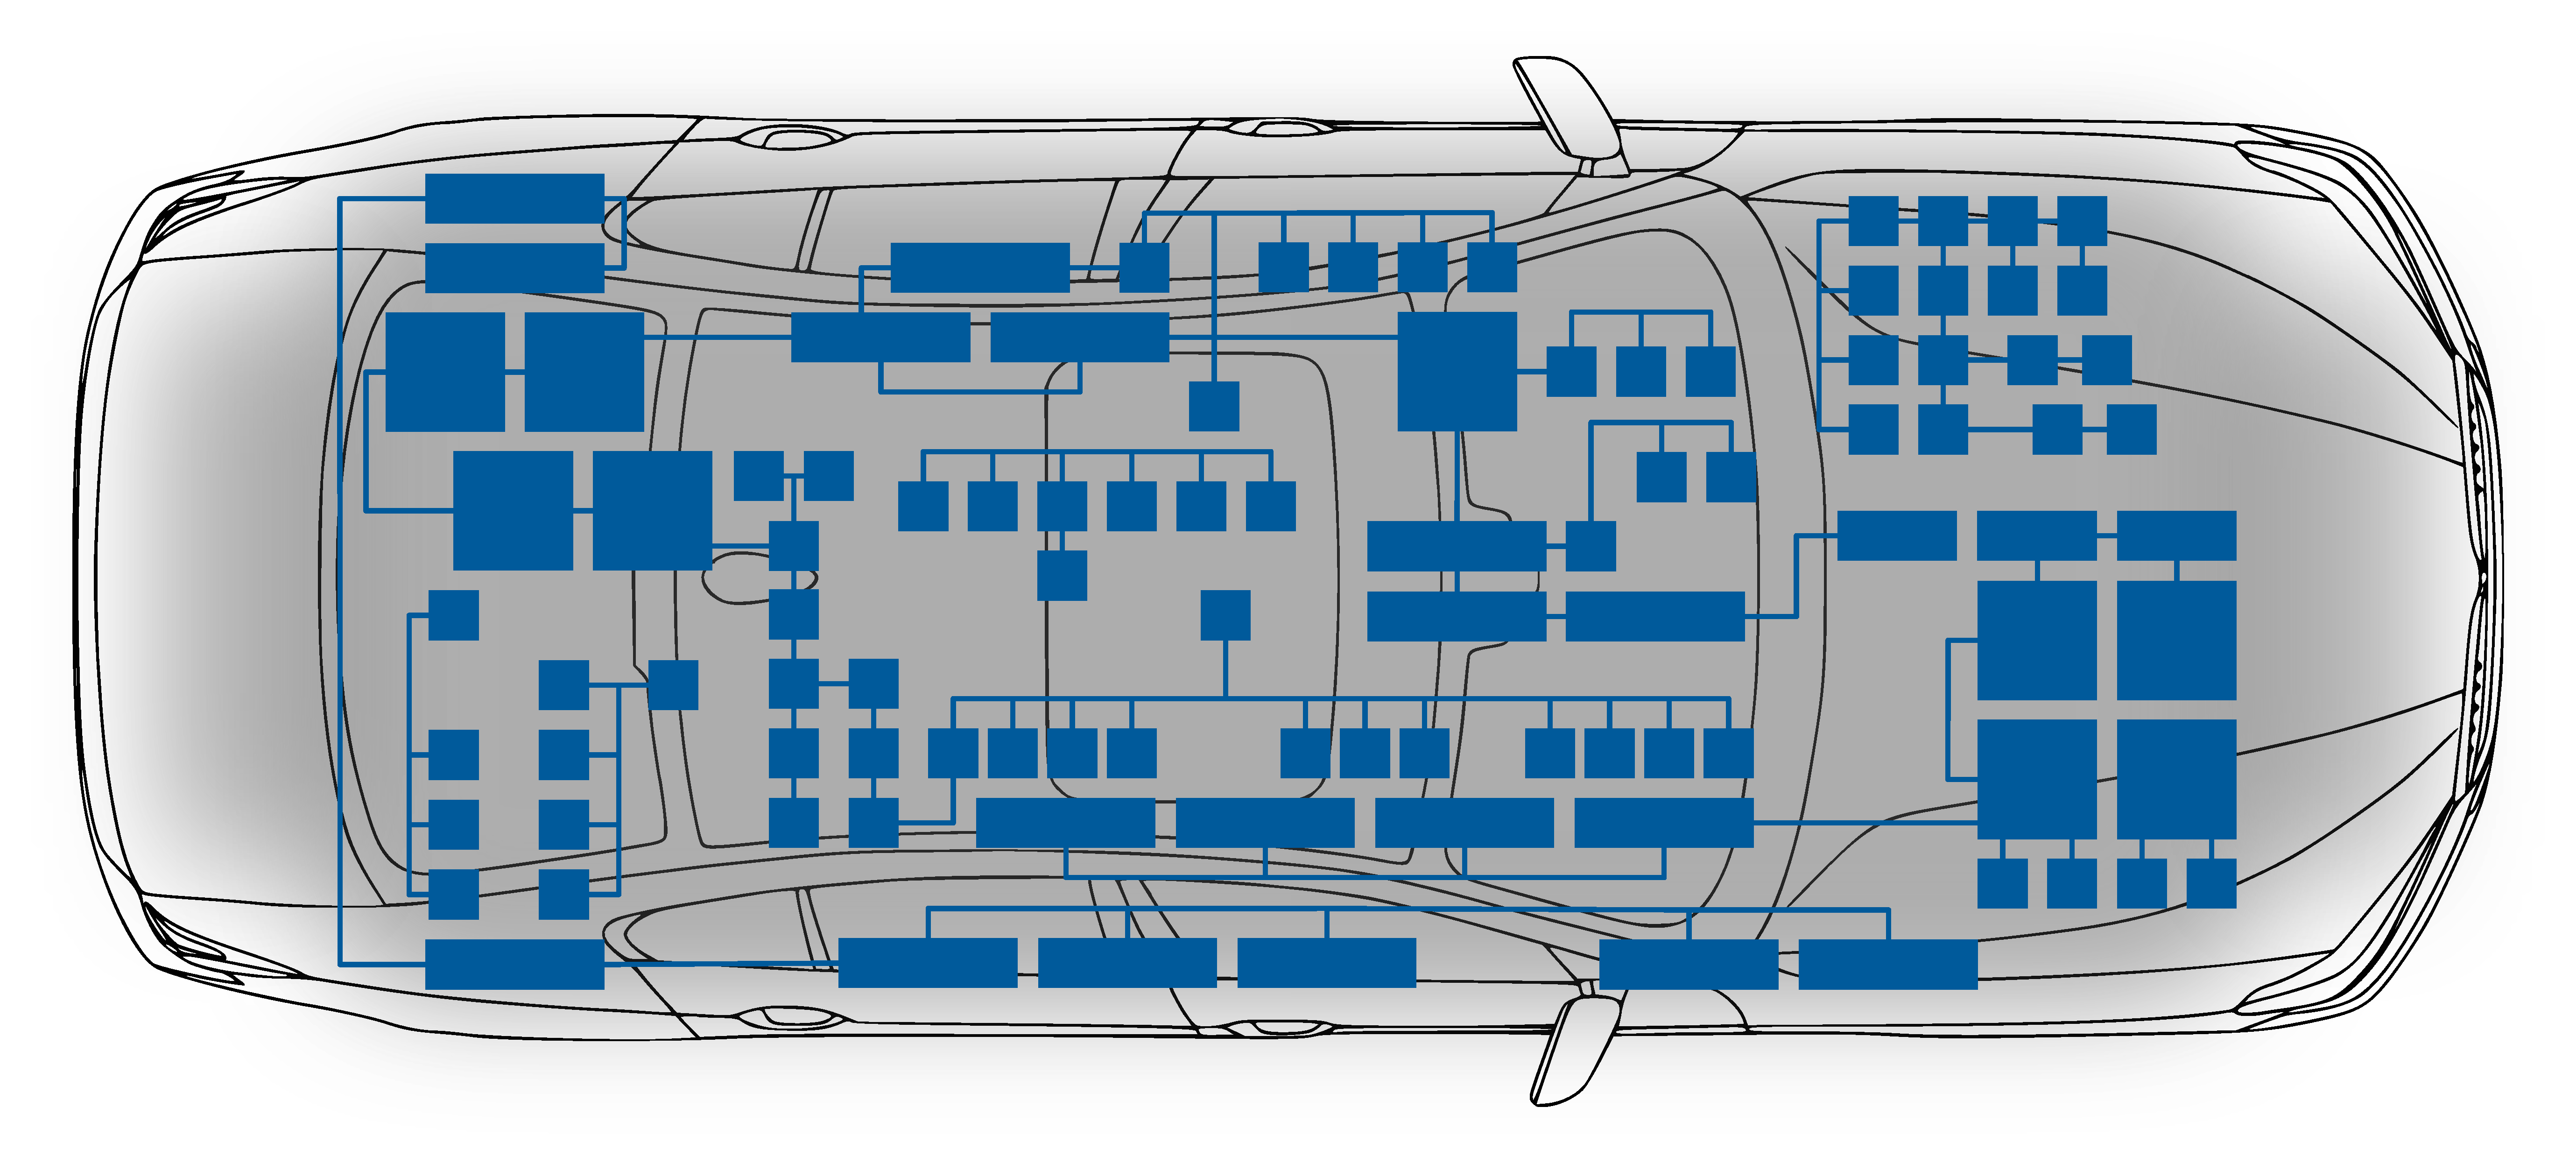
\includegraphics[width=0.9\linewidth]{01_ecu_network.pdf}
            \caption[Schematic ECU distribution in modern vehicles]{Schematic ECU distribution in modern vehicles according to \cite{Bosch2020,Drawingdatabase2020}}
            \label{fig:ecu_network}
        \end{center}
    \end{figure}
    \vfill
   
    
    %----------------------------------------------------------------------------------------
    %	Problem Definition
    %----------------------------------------------------------------------------------------
    \section{Problem Statement}
    \label{section:problem}
    
        \begin{center}
            \begin{minipage}{.9\textwidth}
                \textsl{"Cloud is about how you do computing, not where you do computing."}\\
                {\raggedleft \textsl{$\sim$Paul Maritz, CEO of VMware \cite{Nerdio2016}}\par}
            \end{minipage} 
        \end{center}
        
        \noindent In various disciplines and areas, the future is already  introducing unknown challenges.
        Challenges like autonomous driving or electric vehicles call for new approaches and require rethinking today's situation.
        The increasing demand for computational power and performance contradicts the embedded system characteristics, being very resource-aware and efficient.
        The rising number of \acp{ECU} installed in vehicles already exceeds 100 and makes their management nearly impossible, not even considering the software.
        Through various undertakings towards domain or vehicle centric E/E-Architectures \cite{Zerfowski2019}, the number of \acp{ECU} will decrease, however, multiple \acp{ECU} will still be present in a vehicle.
        Developing software for embedded systems requires engineers not only to solve tomorrow's challenges but also to face more restrictions and environmental factors than in most software development areas.
        Restrictions like cost, weight, or efficiency lead to highly optimized software at the expense of a challenging and complex development process and possibly abandoned functionality.
        
        \noindent To manage requirements and standardize automotive software development, Autosar plays an important role.
        Nevertheless, with the Autosar Classic documentation consisting of over 20.000 pages in the latest release, the standard's complexity is exploding.
        While Autosar enables the development of applications and functionality independently from the hardware, from a certain point, the software has to be statically assigned to specific hardware and, therefore, \acp{ECU}.
        As Paul Maritz said, today's challenges force us to concentrate on the problem itself and on the \textsl{how} we compute rather than concern ourselves with the \textsl{where} we compute.
        With the high number of \acp{ECU}, the rising software quantity and complexity, along with casual embedded system constraints and safety requirements, concentration on the \textsl{where} often shadows the \textsl{how}.
        
        \noindent Figure \ref{fig:ecu_pooling_today} depicts schematically how applications are currently assigned to particular \acp{ECU}.
        Cloud Computing already addresses these static assignations through a middleware representing separate, distributed systems as one pool of shared resources.
        Although Cloud Computing is used in many areas, including the automotive backend, it is yet to be used inside the vehicle.
        Using a middleware that virtualizes and provisions resources to \acp{VM} could facilitate the distribution of applications and software among multiple \acp{ECU}, as depicted by Figure \ref{fig:ecu_pooling_vision}, and overcome the static assignations.
        
        \begin{figure}[ht]
        \centering
            \begin{subfigure}[b]{0.45\textwidth}
                \centering
                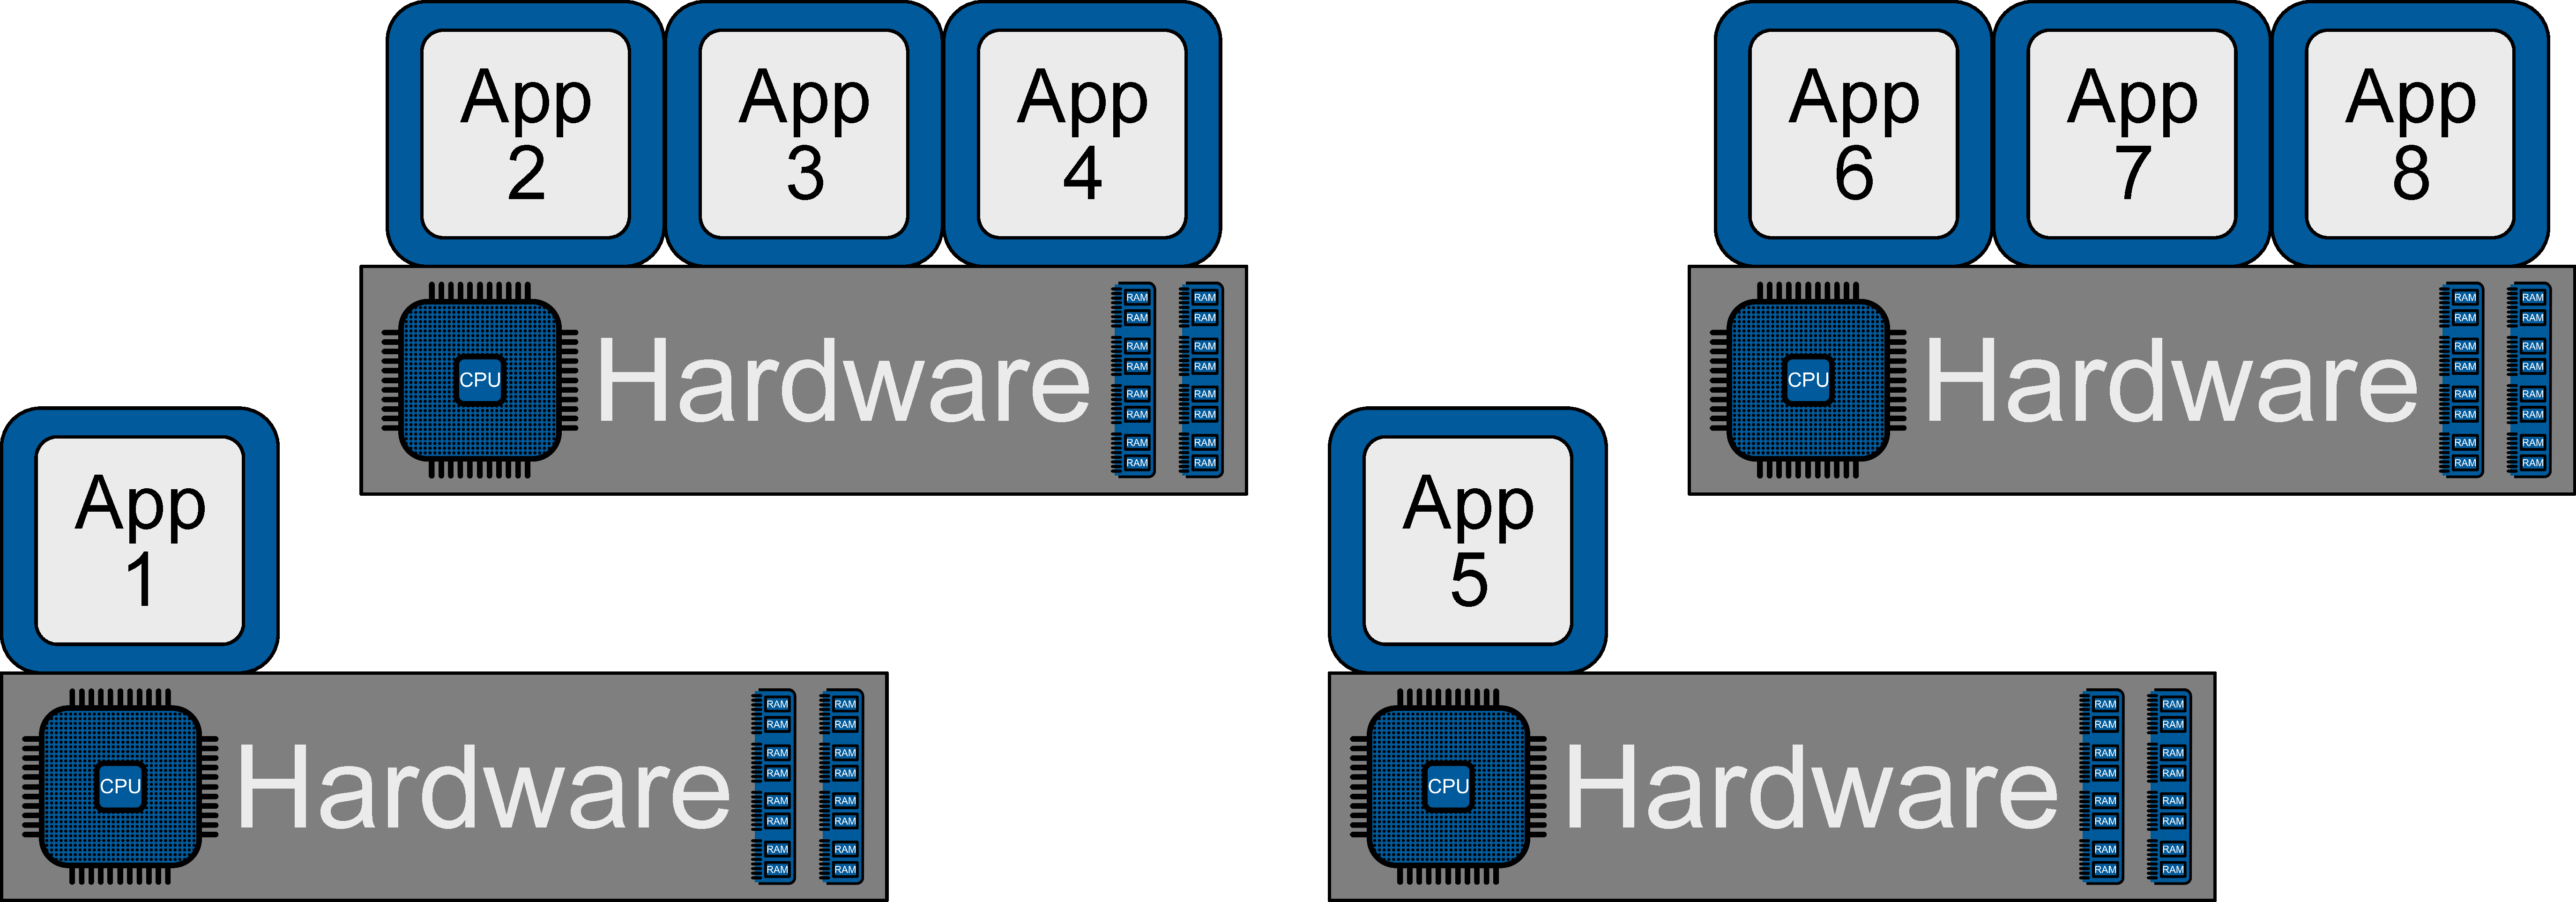
\includegraphics[width=\textwidth]{01_ecu_to_cloud_1.pdf}
                \caption{Today: Applications $\to$ Hardware}
                \label{fig:ecu_pooling_today}
            \end{subfigure}
            \hfill
            \begin{subfigure}[b]{0.45\textwidth}
                \centering
                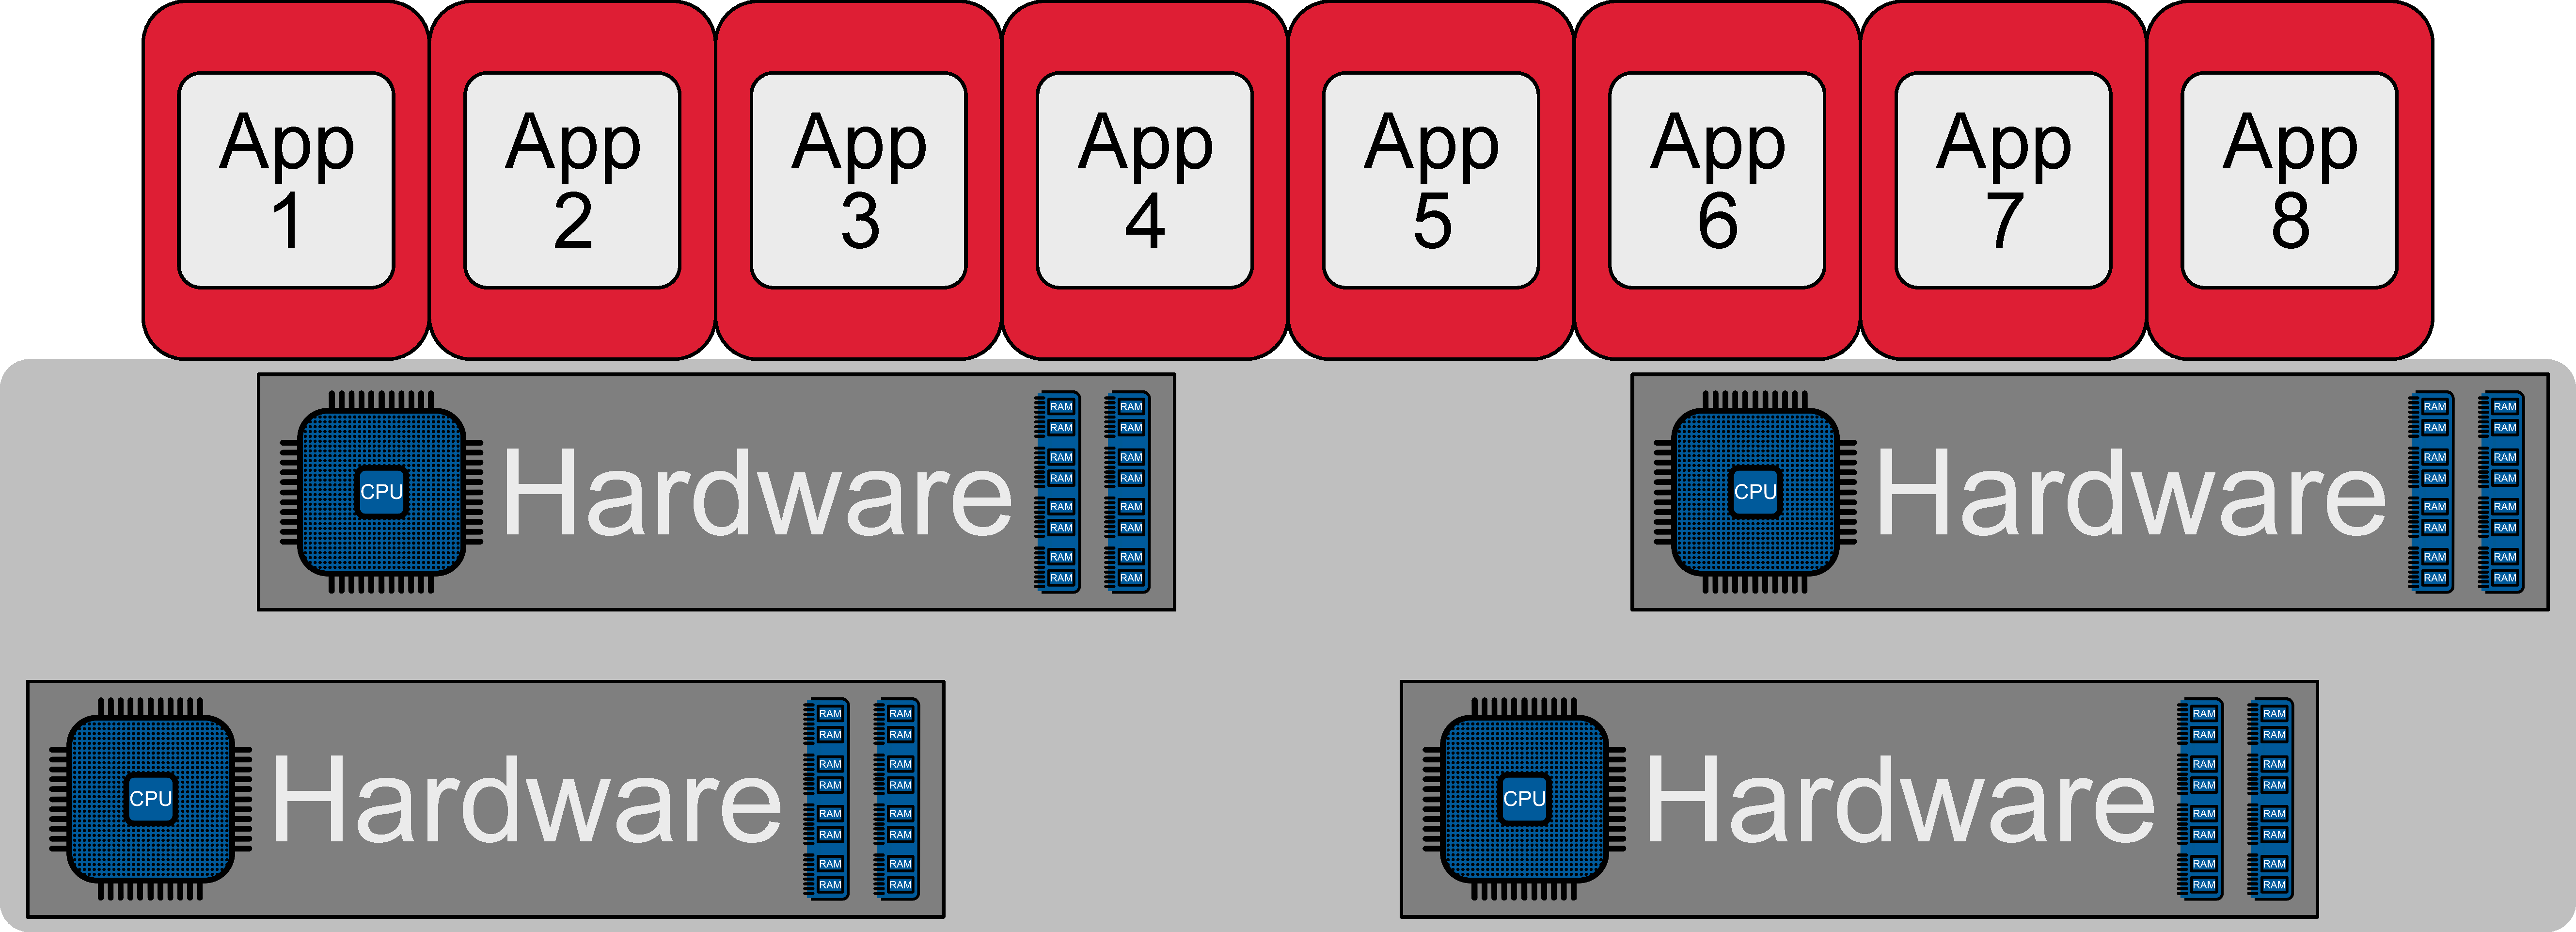
\includegraphics[width=\textwidth]{01_ecu_to_cloud_2.pdf}
                \caption{Vision: Applications $\to$ Shared Pool}
                \label{fig:ecu_pooling_vision}
            \end{subfigure}
            \caption{Symbolic depiction of distributed and pooled resources}
            \label{figure:ecu_pooling}
        \end{figure}

           
    %----------------------------------------------------------------------------------------
    %	Problem Definition
    %----------------------------------------------------------------------------------------
    \section{Goals and Research Question}
    \label{section:problem}
        
        \noindent Providers of Cloud Computing services like Amazon with Amazon Web Services or Microsoft with Microsoft Azure only provide the actual services.
        In contrast, the Open-Source project OpenStack \cite{OpenStack2021} aims at providing all the necessary tools and software to create an own cloud infrastructure.
        With OpenStack, one can deploy a cloud infrastructure on any hardware with sufficient resources.
        This thesis focuses on using OpenStack and its software components for providing computational resources on \acp{SoC} in embedded systems. 
        Therefore, the goal of the thesis presented shall be the successful execution of an OpenStack cluster on automotive embedded hardware.
        However, OpenStack's primary target hardware are servers in data centers.
        By consolidating different hardware into one OpenStack cluster, all resources can be pooled, represented as one shared pool, and provisioned to applications inside \acp{VM}.
        While embedded systems represent an area with specific requirements, OpenStack is developed for typical server environments.
        These contrasts and contradictions have an impact on the use of OpenStack on embedded systems.
        The extent of this impact shall be the research object of this thesis.
        Therefore, the main research question is:

        \begin{center}
            \textbf{Is it possible to leverage the advantages of Cloud Computing on embedded hardware?}
        \end{center}
        
        \noindent This question can be further divided into the following goals:
        \begin{enumerate}
            
            \item \textbf{Install and execute OpenStack on embedded automotive hardware.}\\
            As neither OpenStack is intended for embedded hardware, nor embedded hardware is intended for software like OpenStack, the installation has to be successful prior to actual evaluation.
            Due to custom \acp{OS} and kernels, as well as limited resources, the installation might pose difficulties.
            
            \item \textbf{Determine the impacts of Cloud Computing on embedded systems.}\\
            Due to neither working in the typical data center environment nor working with typical embedded software, special requirements and environmental constraints for OpenStack are present.
            It has to be determined how the contradictory requirements affect the embedded system and also OpenStack.
            On the other hand, it has to be determined whether and which Cloud Computing advantages can be leveraged on embedded systems.
            
            \item \textbf{Measure and evaluate identified impacts.}\\
            Having determined the positive and negative impacts of Cloud Computing, these have to be objectively quantified.
            To evaluate whether the impacts are substantial or negligible, measurements have to be performed in a defined way.
            
            \item \textbf{Evaluate OpenStack's performance on embedded hardware.}\\
            With impacts and their metrics defined, a cloud infrastructure on embedded hardware can be evaluated.
            Executing tests for the relevant metrics enables an assertion on OpenStack's performance on embedded hardware.

        \end{enumerate}
    
    
    %----------------------------------------------------------------------------------------
    %	Structure
    %----------------------------------------------------------------------------------------
    \section{Structure of this Thesis}
    \label{section:structure}
        
        The answer to the main research question is elaborated along the following structure:
        First, Chapter \ref{chapter:basics} establishes the basics in, for this thesis, relevant areas.
        Second, in Chapter \ref{chapter:host_and_Test_setup}, the preparation of the hardware used for the testing and the installation process of OpenStack itself is described.
        In Chapter \ref{chapter:methodology}, the test methodology for accessing OpenStack's overhead is presented, followed by the discussion of the results in Chapter \ref{chapter:measurements}.
        Chapter \ref{chapter:usecases} further examines two exemplary use cases as advantages of OpenStack, leading to a conclusion and outlook in Chapter \ref{chapter:conclusion}.

    

\chapter{Basics}
\label{chapter:basics}
    
    In order to reach the defined goals of this thesis, more profound knowledge in different areas is necessary.
    Besides Cloud Computing and virtualization, common characteristics and features of embedded systems should be known as well.
    Also, familiarization and understanding of OpenStack are crucial.    
    This chapter aims at establishing the fundamentals needed to understand this thesis.
    
    
    %----------------------------------------------------------------------------------------
    %	Cloud Computing
    %----------------------------------------------------------------------------------------
    \section{Cloud Computing}
    \label{section:cloud}
        
        Considering the importance and extensive usage of Cloud Computing in today's world, it is hard to define the exact meaning.
        In 2011, the \ac{NIST} defined \textsl{Cloud Computing} in a special publication. 
        According to \ac{NIST}, Cloud Computing enables \textsl{"ubiquitous, convenient, on-demand network access to a shared pool of configurable computing resources (e.g., networks, servers, storage, applications, and services) that can be rapidly provisioned and released with minimal management effort or service provider interaction"} \cite{Mell2011}.
        Due to the broad utilization of Cloud Computing through third parties like Amazon or Microsoft, terms like pay-as-you-go or payment, in general, are often perceived as part of the definition \cite{Repschlager2010,Amazon2020}.
        Although this often applies, strictly reviewing, Cloud Computing only refers to the provisioning of resources.
        The business models of companies do not relate to the concept itself.
        
        \noindent Additionally, in \cite{Mell2011} \ac{NIST} established five essential characteristics of Cloud Computing.
        Through \textsl{on-demand self-service} and \textsl{broad network access}, consumers can provision computing capabilities without human interaction over the network.
        The providers' \text{resource pooling} allows serving computing resources to multiple consumers.
        \textsl{Rapid elasticity} and a \textsl{measured service} automatically control and optimize resource use by elastically provisioning and releasing them.
        
        \subsection{Service Models}
        \label{subsection:models}
        
            As mentioned previously, the main component of Cloud Computing is the provisioning of resources.
            This provisioning can be done on different levels, enabling different possibilities for the user.
            \ac{NIST} defined the following three service models for Cloud Computing, depicted by Figure \ref{figure:cloud_service_models}.
            
            \noindent \textbf{\ac{SaaS}} 
            As the name suggests, only the software is provisioned.
            In this model, the software is executed on cloud infrastructure and consumers can access it through thin-client interfaces like web browsers.
            The consumers do not manage or even have access to the underlying cloud infrastructure or the environment like the \ac{OS}.
            
            \noindent \textbf{\ac{PaaS}} 
            The service provisioned here is a platform for deployment of applications.
            The provider offers control over deployed applications and possibly over environmental settings for hosting applications.
            The consumers do not manage or even have access to the underlying cloud infrastructure.
            
            \noindent \textbf{\ac{IaaS}} 
            The consumer has access to fundamental computing resources and is able to provision them.
            The user has no access or control over the underlying hardware but can run arbitrary software and control the \ac{OS}, storage, and deployed applications.
            This thesis aims at establishing an \ac{IaaS} cloud on the automotive hardware presented in Chapter \ref{chapter:host_and_Test_setup} using OpenStack.
            
            \begin{figure}[ht]
                \begin{center} 
                    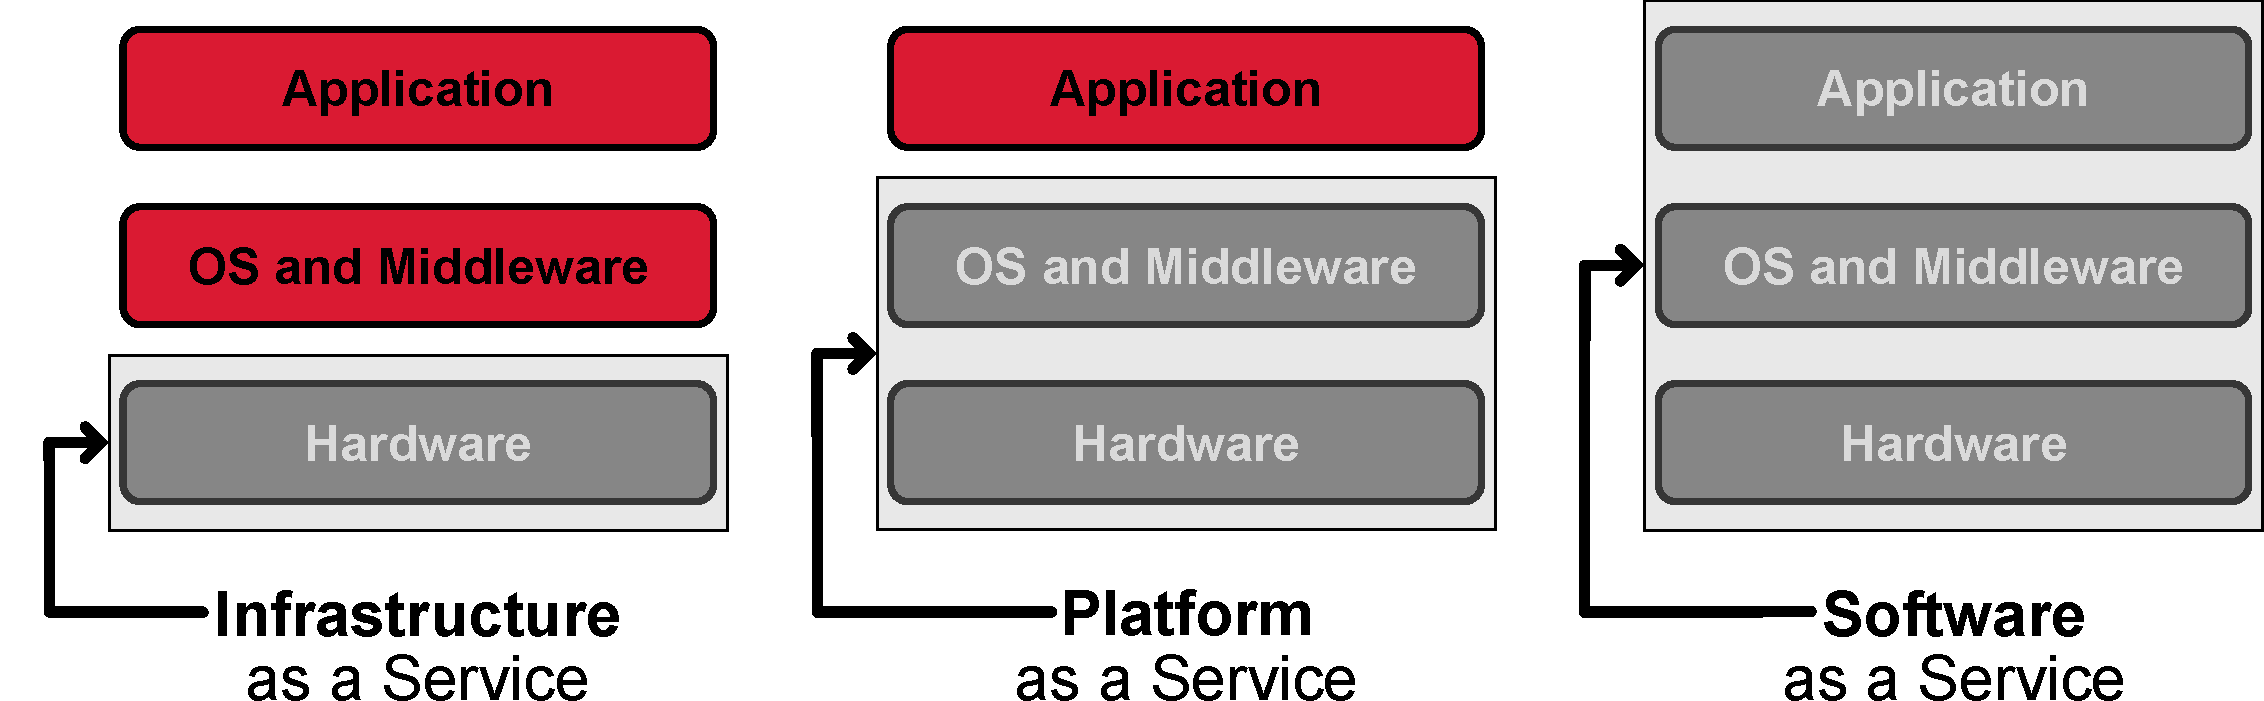
\includegraphics[width=\textwidth ]{02_service_models.pdf} 
                    \caption{Cloud computing service models}
                    \label{figure:cloud_service_models}
                \end{center}	
            \end{figure}
        
        
        \subsection{Architectures}
        \label{subsection:architecture}
            
            Except for different service models, Cloud Computing can be characterized by its architecture.
            Depending on the accessibility to the infrastructure, the following architectures are defined.
            
            \newpage
            \noindent \textbf{Private Cloud} 
            The infrastructure is available for only one organization.
            Related consumers, e.g., business units, can access and use the infrastructure.
            The infrastructure itself can be managed either by the organization itself, a third party, or a combination of both.
            Throughout this thesis, a private architecture is used, as no access for other parties is considered.
            
            \noindent \textbf{Community Cloud}
            In addition to private clouds, in community clouds, the usage is not exclusive to one organization.
            Organizations with shared interests and concerns have access to the infrastructure and can access the provided services.
            The infrastructure itself can be managed by either one of the organizations itself, a third party, or a combination of both.
            
            \noindent \textbf{Public Cloud}
            As the name suggests the cloud infrastructure is accessible by the general public for use.
            Various institutions, like businesses, academics, or governments, can be responsible for managing the cloud infrastructure.
            
            \noindent \textbf{Hybrid Cloud} 
            This infrastructure is a composition of two or more different cloud infrastructures.
            Both clouds remain unique entities but are connected to each other for, for example, data exchange.
            
        \subsection{Advantages and Disadvantages}
        \label{subsection:advantages_disadvantages}
            
            Cloud Computing is not without reason a prevalent and beneficial model.
            Various reasons exist why Cloud Computing should be adopted, from a technical and business point of view.
            However, Cloud Computing also comes with negative aspects, especially for embedded systems.
            Based on \cite{Alzahrani2014,Hallmans2015}, some advantages and disadvantages of Cloud Computing shall be pointed out.
            
            
            \subsubsection{Advantages}
            
                \noindent Cloud Computing introduces a new degree of \textbf{flexibility}. 
                Virtualizing available, distributed resources as one coherent pool makes the allocation of applications to specific systems like a specific \ac{ECU} redundant.
                
                \noindent Moreover, \textbf{scalability} and, therefore, \textbf{performance} can be tremendously improved.
                Regarding the topic of upgradability, in current embedded systems, this is not even considered or possible. 
                Through Cloud Computing, upgrading or simply adding resources, for example, computing power or memory, would instantaneously become possible. 
                Especially in today's environmentally and resource-conscious society, this could be an interesting topic.
                
                \newpage
                \noindent Additionally, Cloud Computing is ideal if \textbf{redundancy} is needed.
                Considering embedded systems with high safety requirements, this is essential.
                While today additional hardware is used, Cloud Computing could enable applications to be easily shifted or duplicated in case of hardware failure.
                Chapter \ref{chapter:usecases} examines the advantages of flexibility and redundancy in greater detail.
            
             
            \subsubsection{Disadvantages}
            
                \noindent Deploying and managing cloud infrastructures introduces a significant level of \textbf{complexity}.
                Understanding the exact behavior of the whole software or software components becomes impossible.
                
                \noindent This introduces new problems in the areas of \textbf{security}.
                Especially for embedded systems, where updating software is not necessarily intended, security flaws and vulnerabilities are critical.
                With big and complex software, vulnerabilities can be overlooked and later discovered during production.
                While in data centers, this can quickly be resolved through updates, embedded systems are scarcely updated.
                Using cloud infrastructure could therefore create a conflict with this tradition
                
                \noindent Further, this contradicts embedded systems with high safety requirements that must have \textbf{deterministic behavior}.
                Besides the inability to understand the whole software, possible exploitation of security flaws adds to the fact that it is impossible to know the software's behavior with confidence. 
            
    
    %----------------------------------------------------------------------------------------
    %	Virtualization
    %----------------------------------------------------------------------------------------
    \section{Virtualization}
    \label{section:virtualization}
    
        Cloud Computing relies on the provisioning of resources. 
        To do that, resources like the \ac{CPU}, \ac{CPU} cycles, or memory have to be virtualized.
        Virtualization describes a real-world object's mapping onto a virtual object with the same or similar properties \cite{Garbacki2007}.
        This allows applications and services to be deployed onto the virtualized hardware instead of directly onto the physical resources.
        From now on, the hardware providing the resources is called the \textsl{host}, while the software, for example, a \ac{VM}, using those resources is called the \textsl{guest}.
        The management of the virtualized resources is handled by a software called \textsl{hypervisor}.
        The following subsections will describe two common concepts of virtualization, as well as two common hypervisors using these concepts.
        
        
        \subsection{Hypervisors}
        \label{subsection:hypervisors}
        
            Hypervisors are systems or pieces of software initially developed for monitoring purposes in virtual computing \cite{Blenk2016}.
            In addition, hypervisors are responsible for the allocation of physical resources to individual guests.
            Guest \acp{VM}, for example, can execute their own \ac{OS} and run as an individual computing platform.
            By providing a hardware abstraction layer, hypervisors provide interfaces for guests to interact with the physical hardware.
            Two widely used hypervisors are \ac{KVM} and XEN.
            In this thesis, the OpenStack cluster will use \ac{KVM} as the hypervisor.
        
        
        \subsection{Virtualization Concepts}
        \label{subsection:concepts}
        
            For the virtualization of resources, especially the \ac{CPU} and \ac{CPU} cycles, two main approaches established themselves.
            Their main difference resides in the hypervisor and the hypervisors reaction to non-virtualizable machine instructions.
            During execution, atomic machine instructions define the actions performed by the processor. 
            While most machine instructions are independent of specific architectures, some instructions behave differently or require specific privileges \cite{Marinescu2018}.
            As stated by Popeck and Goldberg already in 1974, to provide efficient behavior to guests, a certain percentage of instructions must be executed without the hypervisors intervention \cite{Popek1974}.
            In cases where hypervisors' interventions are necessary, the instructions require a specific behavior not known by the hardware. 
            To resolve such non-virtualizable instructions, two different strategies can be used, resulting in two different virtualization approaches visualized by Figure \ref{figure:full_para_virtualization}.
            
            \noindent \textbf{Full-Virtualization} 
            Guests run on a hardware abstraction layer, being an exact copy of the host hardware \cite{Marinescu2018}. 
            In the case of non-virtualizable instructions, the hypervisor identifies these instructions in memory during execution and replaces them with suitable instructions \cite{Binu2011}.
            The guest is not aware of this replacement and continues its execution unhindered.
            Therefore, no modifications need to be performed to the guest system in advance, but the host hardware must support hardware virtualization to provide an efficient solution. 
            \ac{KVM} is a widely adopted hypervisor using full-virtualization.
            
            \noindent \textbf{Para-Virtualization} 
            Guests run on a hardware abstraction layer, being a slightly modified copy of the host hardware \cite{Marinescu2018}. 
            In the case of non-virtualizable instructions, the hypervisor provides a specific interface to the virtualized hardware to translate these instructions \cite{Binu2011}.
            The guest must be extended with specific drivers to make use of this interface.
            Therefore modifications to the guest are needed, but contrary to full-virtualization, para-virtualization does not require hardware support for virtualization.
            XEN is a popular hypervisor using para-virtualization.
            
            \begin{figure}[ht]
                \begin{center} 
                    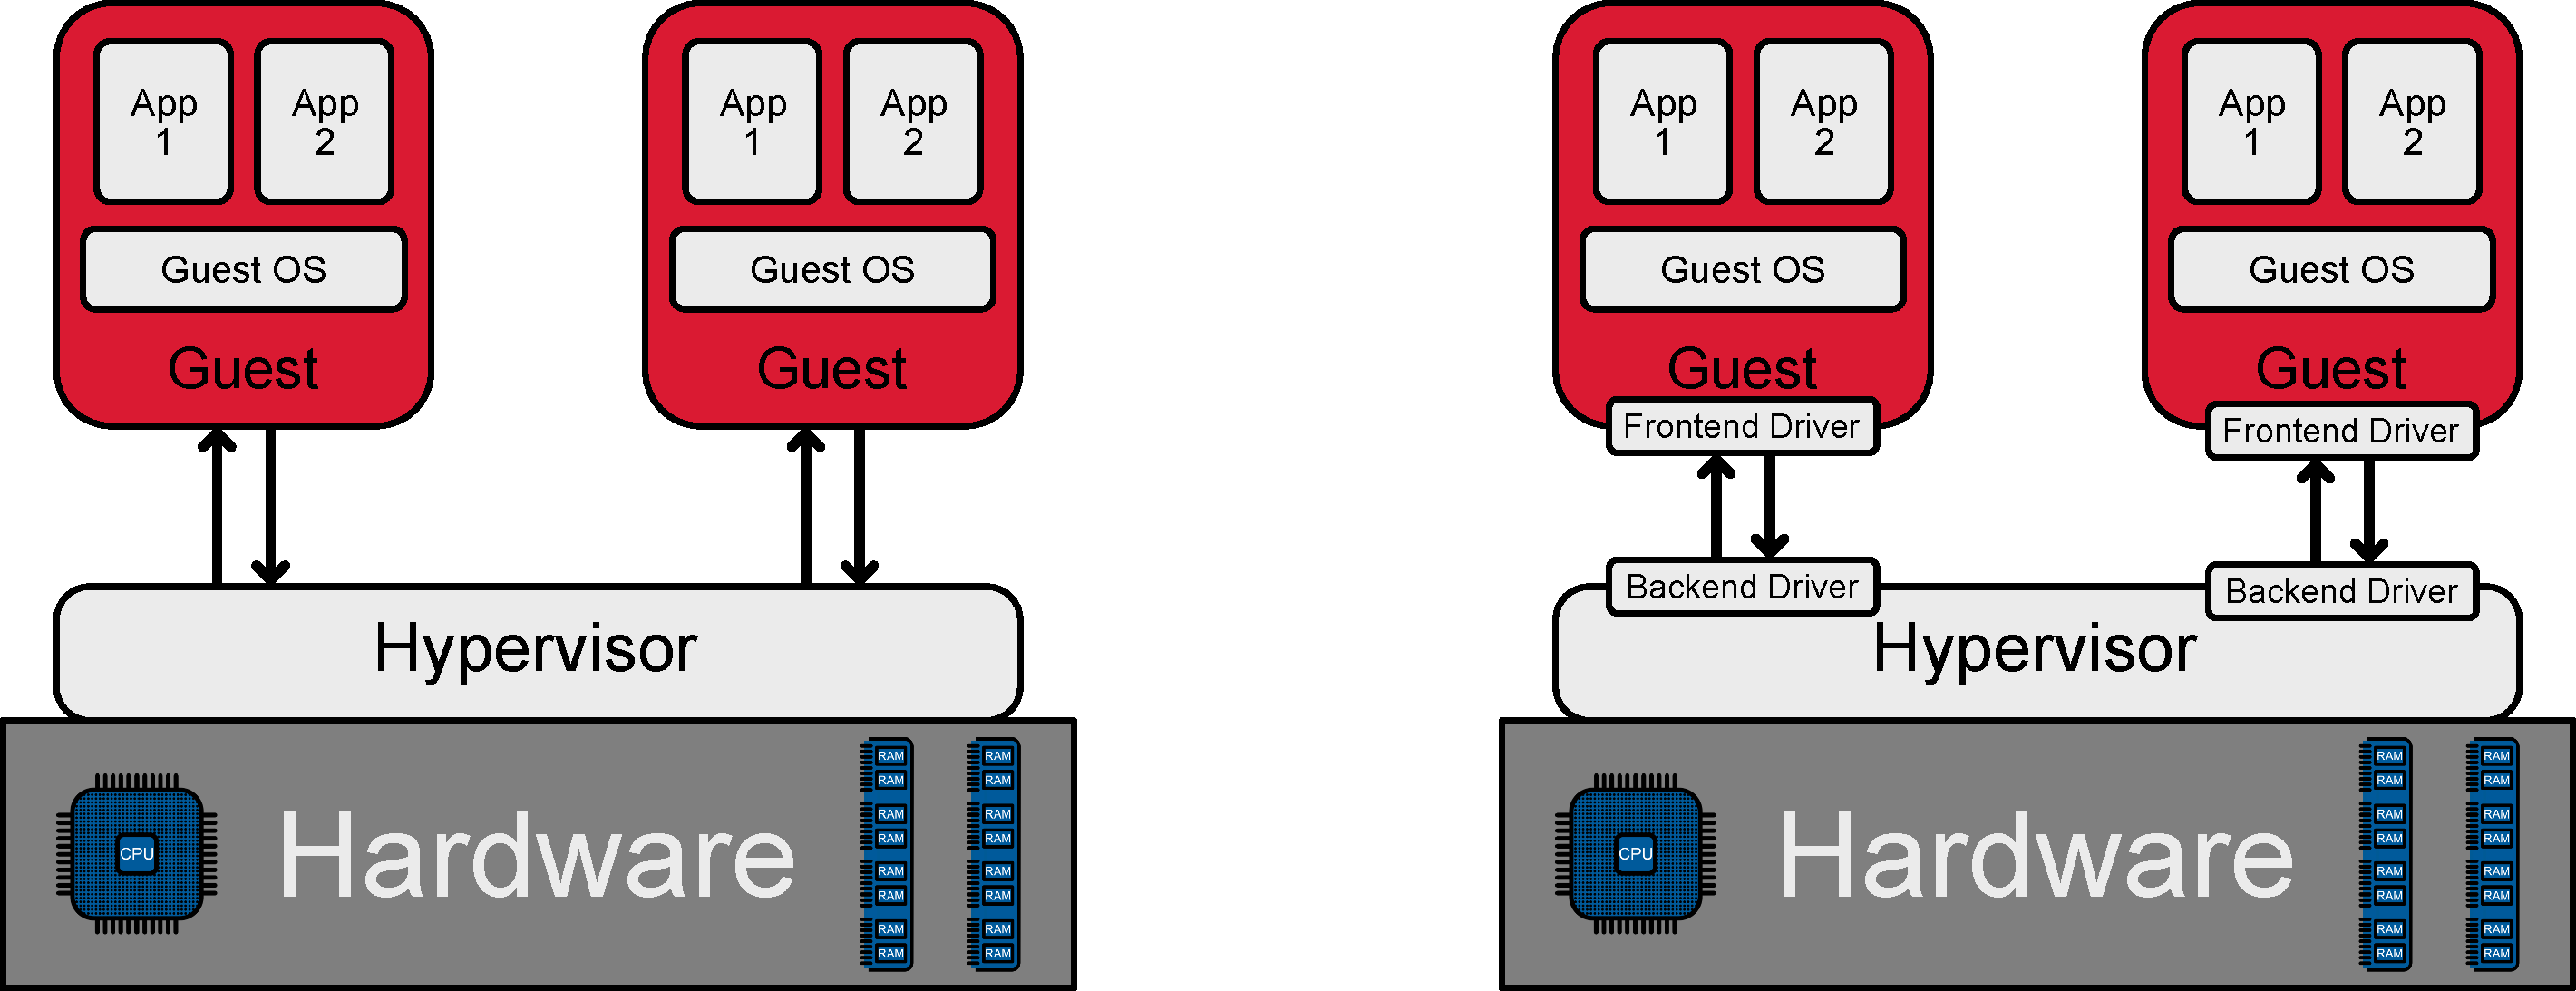
\includegraphics[width=\textwidth]{02_virt_concepts} 
                    \caption[Full-Virtualization and Para-Virtualization]{Full-Virtualization (left)  and Para-Virtualization (right)}
                    \label{figure:full_para_virtualization}
                \end{center}	
             \end{figure}

        
    %----------------------------------------------------------------------------------------
    %	Embedded Systems
    %----------------------------------------------------------------------------------------
    \section{Embedded Systems}
    \label{section:embedded}
    
        In today's world, embedded systems are widely adopted and in use.
        From areas like robotics and the Internet of Things, over automotive and avionic systems to nuclear power plants, embedded systems perform various essential tasks.
        Although these areas all come with different requirements, the function of embedded systems mostly stays the same.
        P. Marwedel defined embedded systems as \textsl{"information processing systems embedded into enclosing products"} \cite{Marwedel2018}.
        Often, embedded systems are linked to the physical world and interact with physical processes.
        In such cases, the systems can be named \textsl{Cyber-Physical Systems}. 
        In \cite{Lee2007}, E. Lee defined Cyber-Physical Systems as \textsl{"integrations of computation and physical processes"}.
        The following sections are based on P. Marwedel's book on Embedded Systems Foundations of Cyber-Physical Systems \cite{Marwedel2018}.
        
        
        \subsection{Characteristics}
        \label{subsection:characteristics}
        
            Despite different environments, embedded systems share several characteristics and challenges these systems have to meet.
            According to P. Marwedel, the following attributes are commonly found:
            
           \noindent \textbf{Dependability} 
            Due to the direct interaction with the environment, embedded systems have an immediate effect and impact on the physical world.
            Additionally, as described later, the lack of a minimal user interface makes a human reaction in case of failure or misbehavior very hard or even impossible.
            Therefore, embedded systems must be dependable by providing safety, security, confidentiality, reliability, maintainability, and availability.
            
           \noindent \textbf{Time Constraints}
            The interaction with physical processes binds the execution or computation of specific things to determined deadlines.
            Depending on the computation and the physical process involved, these limits can be either short or long.
            Moreover, depending on the physical process, a deadline miss can be either catastrophic or less noticeable. 
            
           \noindent \textbf{Resource Awareness}
            Representing not the primary system but being embedded into an encapsulating product, embedded systems often are restricted in various resources.
            Resources like code size and performance or run-time efficiency are optimized as far as possible. 
            Through this, further resources like energy, weight, or space can be optimized.
            Due to very high production volumes of embedded systems, for example, automotive \acp{ECU}, the cost is a crucial factor.
            By minimizing any resource usage, general costs can be reduced, which is very much desirable.            

           \noindent \textbf{Dedicated User Interface}
            The integration into encapsulating products implies that the interaction will most probably happen with the outer product.
            Therefore, user interfaces of embedded systems are specific to the application and held as minimal as possible.
            If no interaction is anticipated, no user interface is provided. 
            Only interfaces for debugging or flashing may then be implemented, consisting of simple switches or interfaces for console access.
        
              
        \subsection{Software}
        \label{subsection:software}
        
            To successfully overcome challenges like time constrains and dependability, \acp{OS} for embedded systems are specially tailored.
            Limited resources and defined applications make it possible and necessary to specifically configure \acp{OS} according to individual needs.
            The lack of untested and unnecessary software allows the assumption about the presence of only reliable and safe software, which further allows to leave out standard protection mechanisms.
            For the embedded environment, access to \ac{OS} service calls or interrupts is essential to react fast and on time to specific events, like sensor data.
            As many embedded systems do not underlie only time constraints but must be real-time capable, further functionality is required by the \ac{OS}.
            
            \noindent \textbf{Real-Time OS}
            Real-Time \acp{OS} are necessary for the construction of real-time systems.
            Real-Time systems describe systems, which not only depend on the functional correctness but equally depend on the in-time computation of results.
            In other words, a particular deadline for a computation must not be missed, or else catastrophic events could occur.
            To ensure such deadlines are not missed, real-time \acp{OS} must provide very predictable timing.
            The OS must manage the scheduling of threads, processes, and tasks through appropriate scheduling algorithms to enable an in-time computation of every task.            
            Naturally, the \ac{OS} must additionally be fast and deliver a good performance.
            These requirements are achieved through the use of fast, customized, and proprietary kernels, as well as with real-time extensions to standard \acp{OS}.
            
            \noindent \textbf{Embedded Linux}
            With more complex applications and more requirements, embedded \acp{OS} must provide increased functionality.
            When developing new software components and integrating them, using an existing and extensively tested \ac{OS} can be preferable.
            Using Linux, which relies on an Open-Source kernel, eliminates commercial costs and allows the kernel's desired configurability.
            The primary target environment for Linux being servers and desktops, Linux is designed for general-purpose computing.
            Aiming for high average performance and fair scheduling, additional scheduling policies must be added to the kernel to satisfy real-time requirements.
            Similarly, the usage of memory differs in desktop and server environments.
            While in desktop and server environments, the memory is often used for caching, this is a waste of resources in the context of embedded systems.
            Although there are techniques to eliminate this duplication of memory, they come at the cost of high complexity and often more expensive storage solutions.
            This again leads to the reconsideration of allowing, for example, swap space and using larger memory.             
   
   
    %----------------------------------------------------------------------------------------
    %	 OpenStack
    %----------------------------------------------------------------------------------------
    \section{OpenStack}
    \label{section:openstack}
        
        OpenStack is a free and Open-Source Cloud Computing software.
        It aims at providing \textsl{"a ubiquitous Open Source Cloud Computing platform that is easy to use, simple to implement, interoperable between deployments, works well at all scales, and meets the needs of users and operators of both public and private clouds”} \cite{OpenStackH2018}.
        In other words, OpenStack enables the deployment of own clouds on the hardware of choice. 
        The project itself originated from two separate projects at Rackspace and Anso Labs, developing both the corresponding counterparts for each other.
        In 2010, the project OpenStack was officially announced and the first release published.
        At the time of writing, 22 releases happened, with the newest one having the series name \textsl{Victoria}.
        This release was used throughout this thesis for all OpenStack software and components.
        
        \noindent OpenStack is built upon multiple different software components, each providing specific functionality.
        Currently, OpenStack consists of 45 different components.
        Figure \ref{figure:openstack_map} shows all available OpenStack software components along with additional software and tools.
        The relevant components for this thesis will be presented in the next section.
        
        \begin{figure}[ht]
            \begin{center} 
                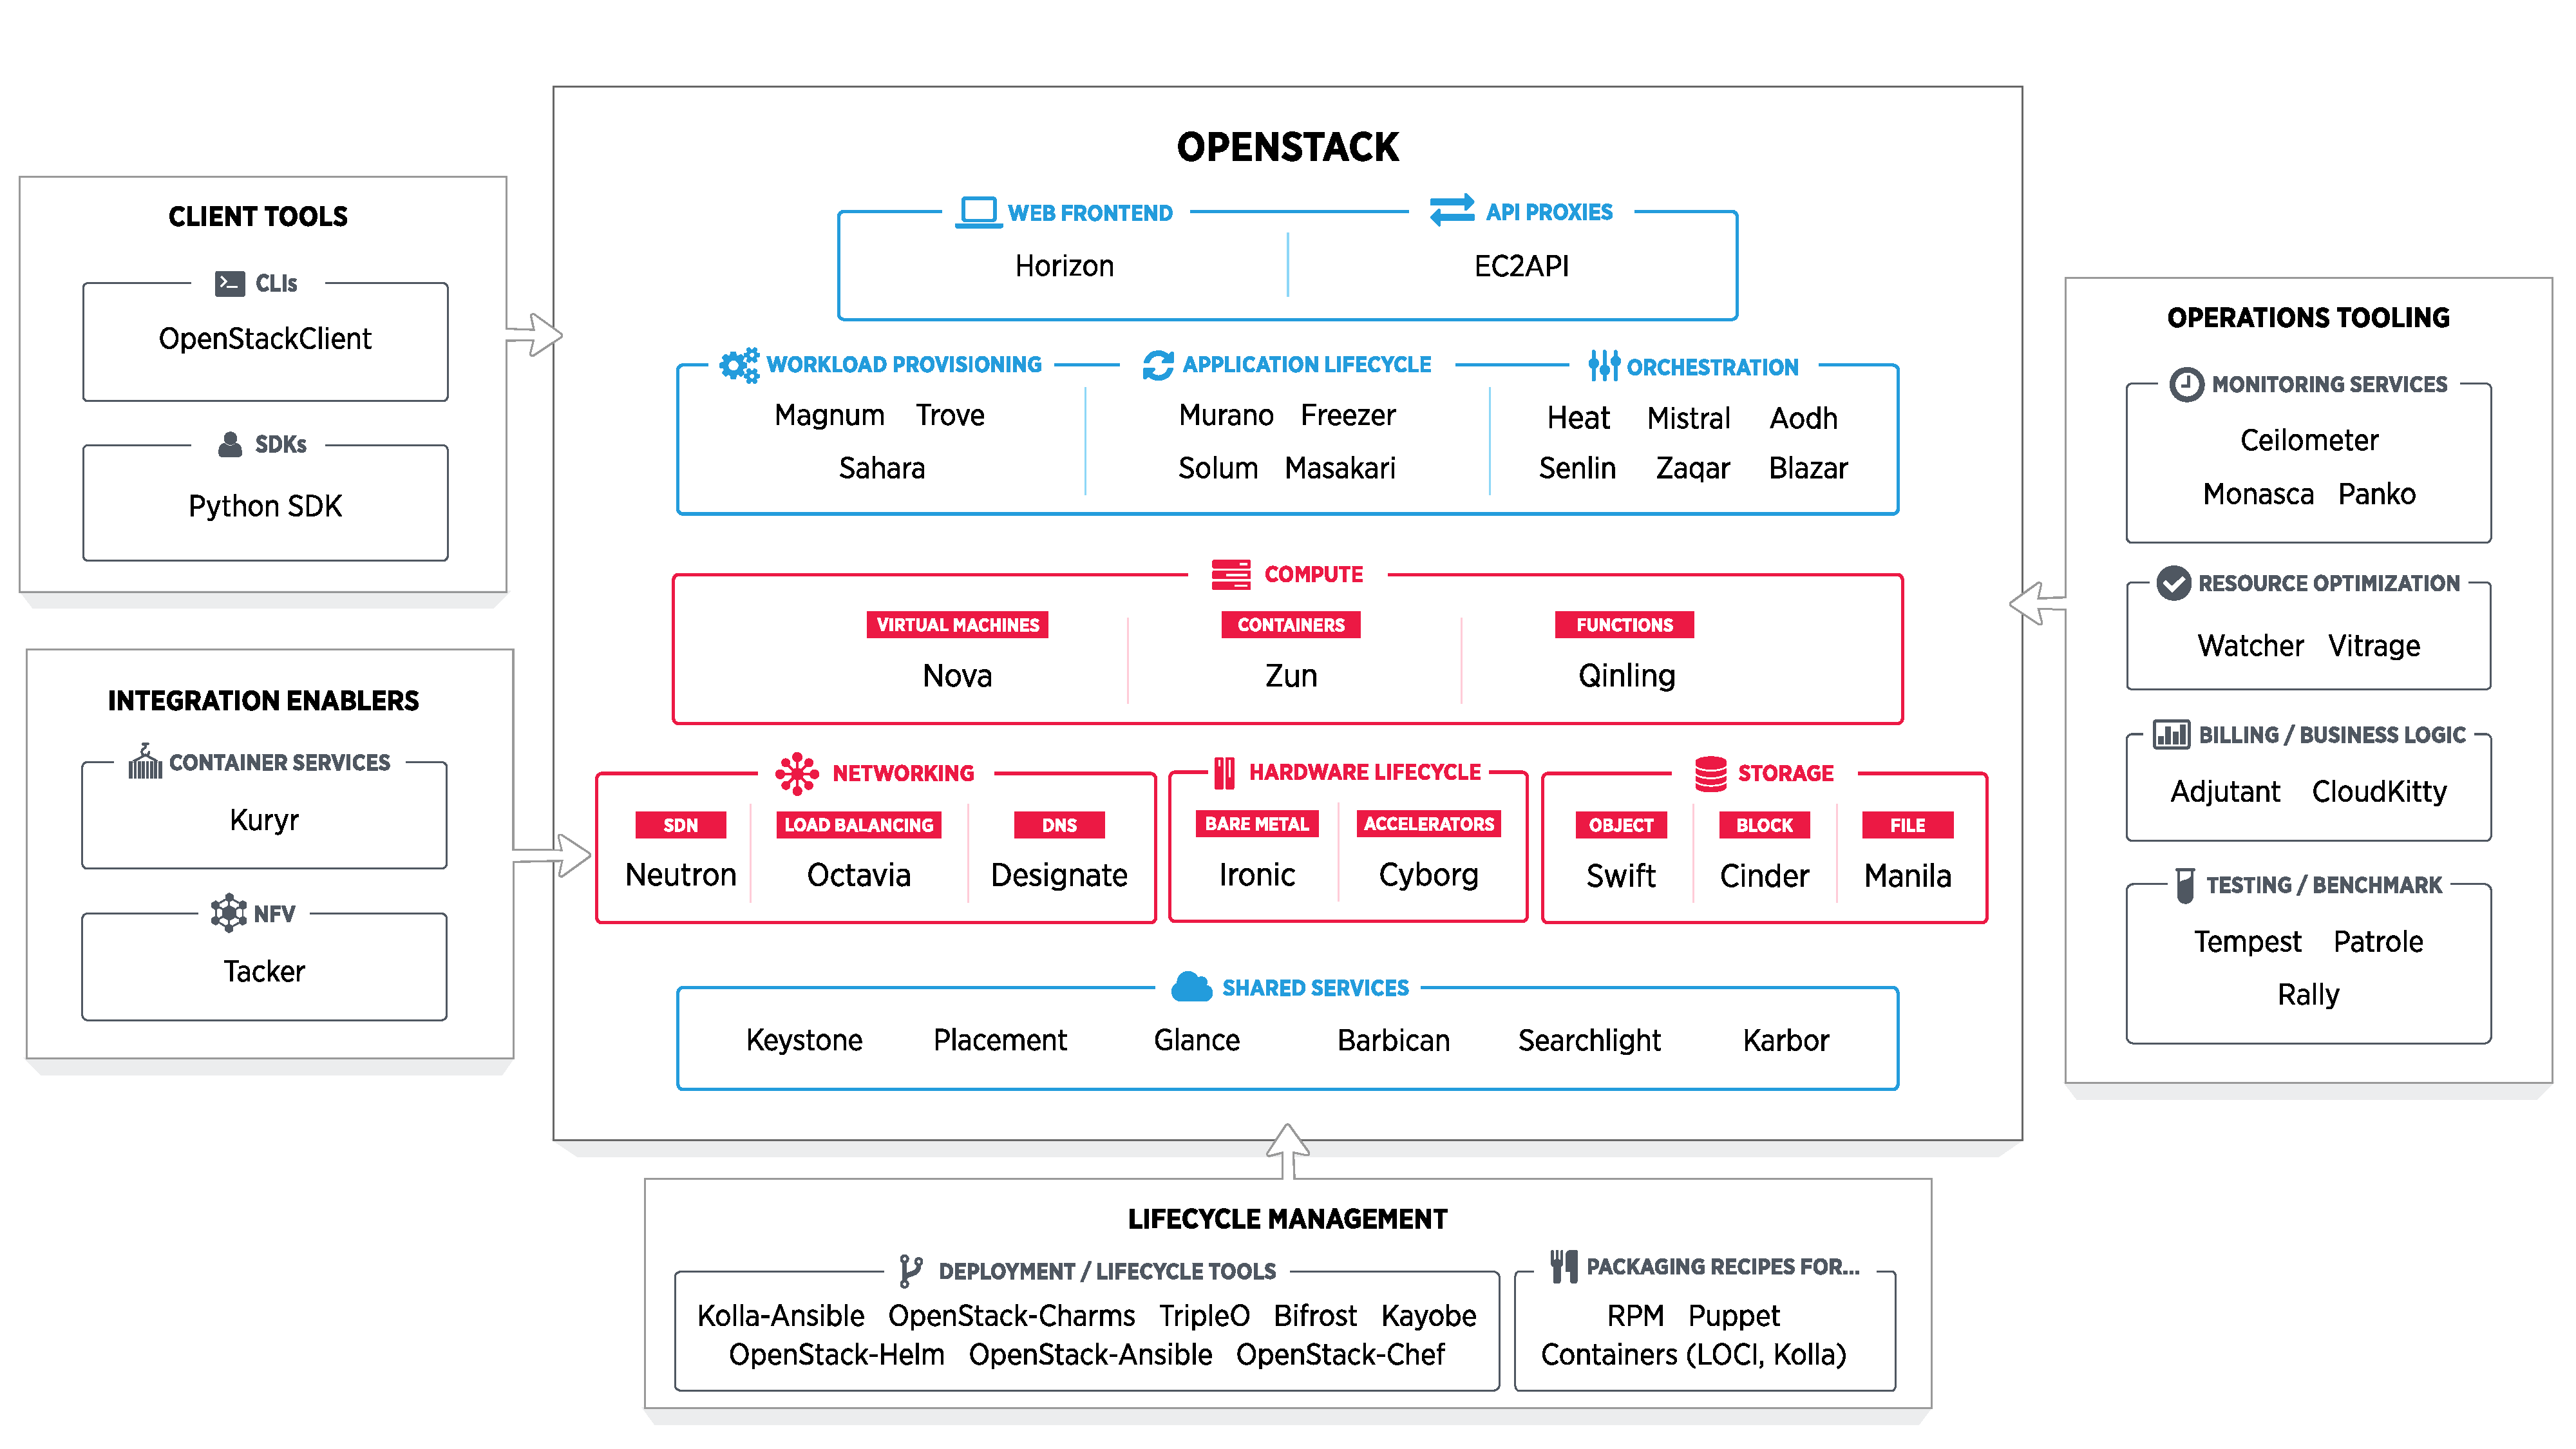
\includegraphics[width=\textwidth ]{02_openstack-map} 
                \caption[Map of OpenStack's software landscape]{Map of the OpenStack's software landscape \cite{OpenStackL2020}}
                \label{figure:openstack_map}
            \end{center}	
         \end{figure}
         
        \noindent With OpenStack's numerous components and their primarily intended environment being data centers, an OpenStack cluster is designed to consist of multiple hosts.
        However, it is possible to install and execute all services on one host.
        Commonly, an OpenStack cluster consists of one controller node and multiple compute nodes.
        Depending on the goals and resources, dedicated storage and networking nodes are possible.
        Throughout this thesis, only dedicated compute nodes will exist, while all other services and components will be executed on one controller node.


        \subsection{Software Components}
        \label{subsection:components}
            
            As depicted in Figure \ref{figure:openstack_map}, many different software components exist.
            For the scope of this thesis, only the crucial components of an OpenStack cluster will be used.
            Figure \ref{figure:openstack_components} illustrates these components along with their interactions.
            The following sections briefly describe these components.
            
            \begin{figure}[ht]
                \begin{center} 
                    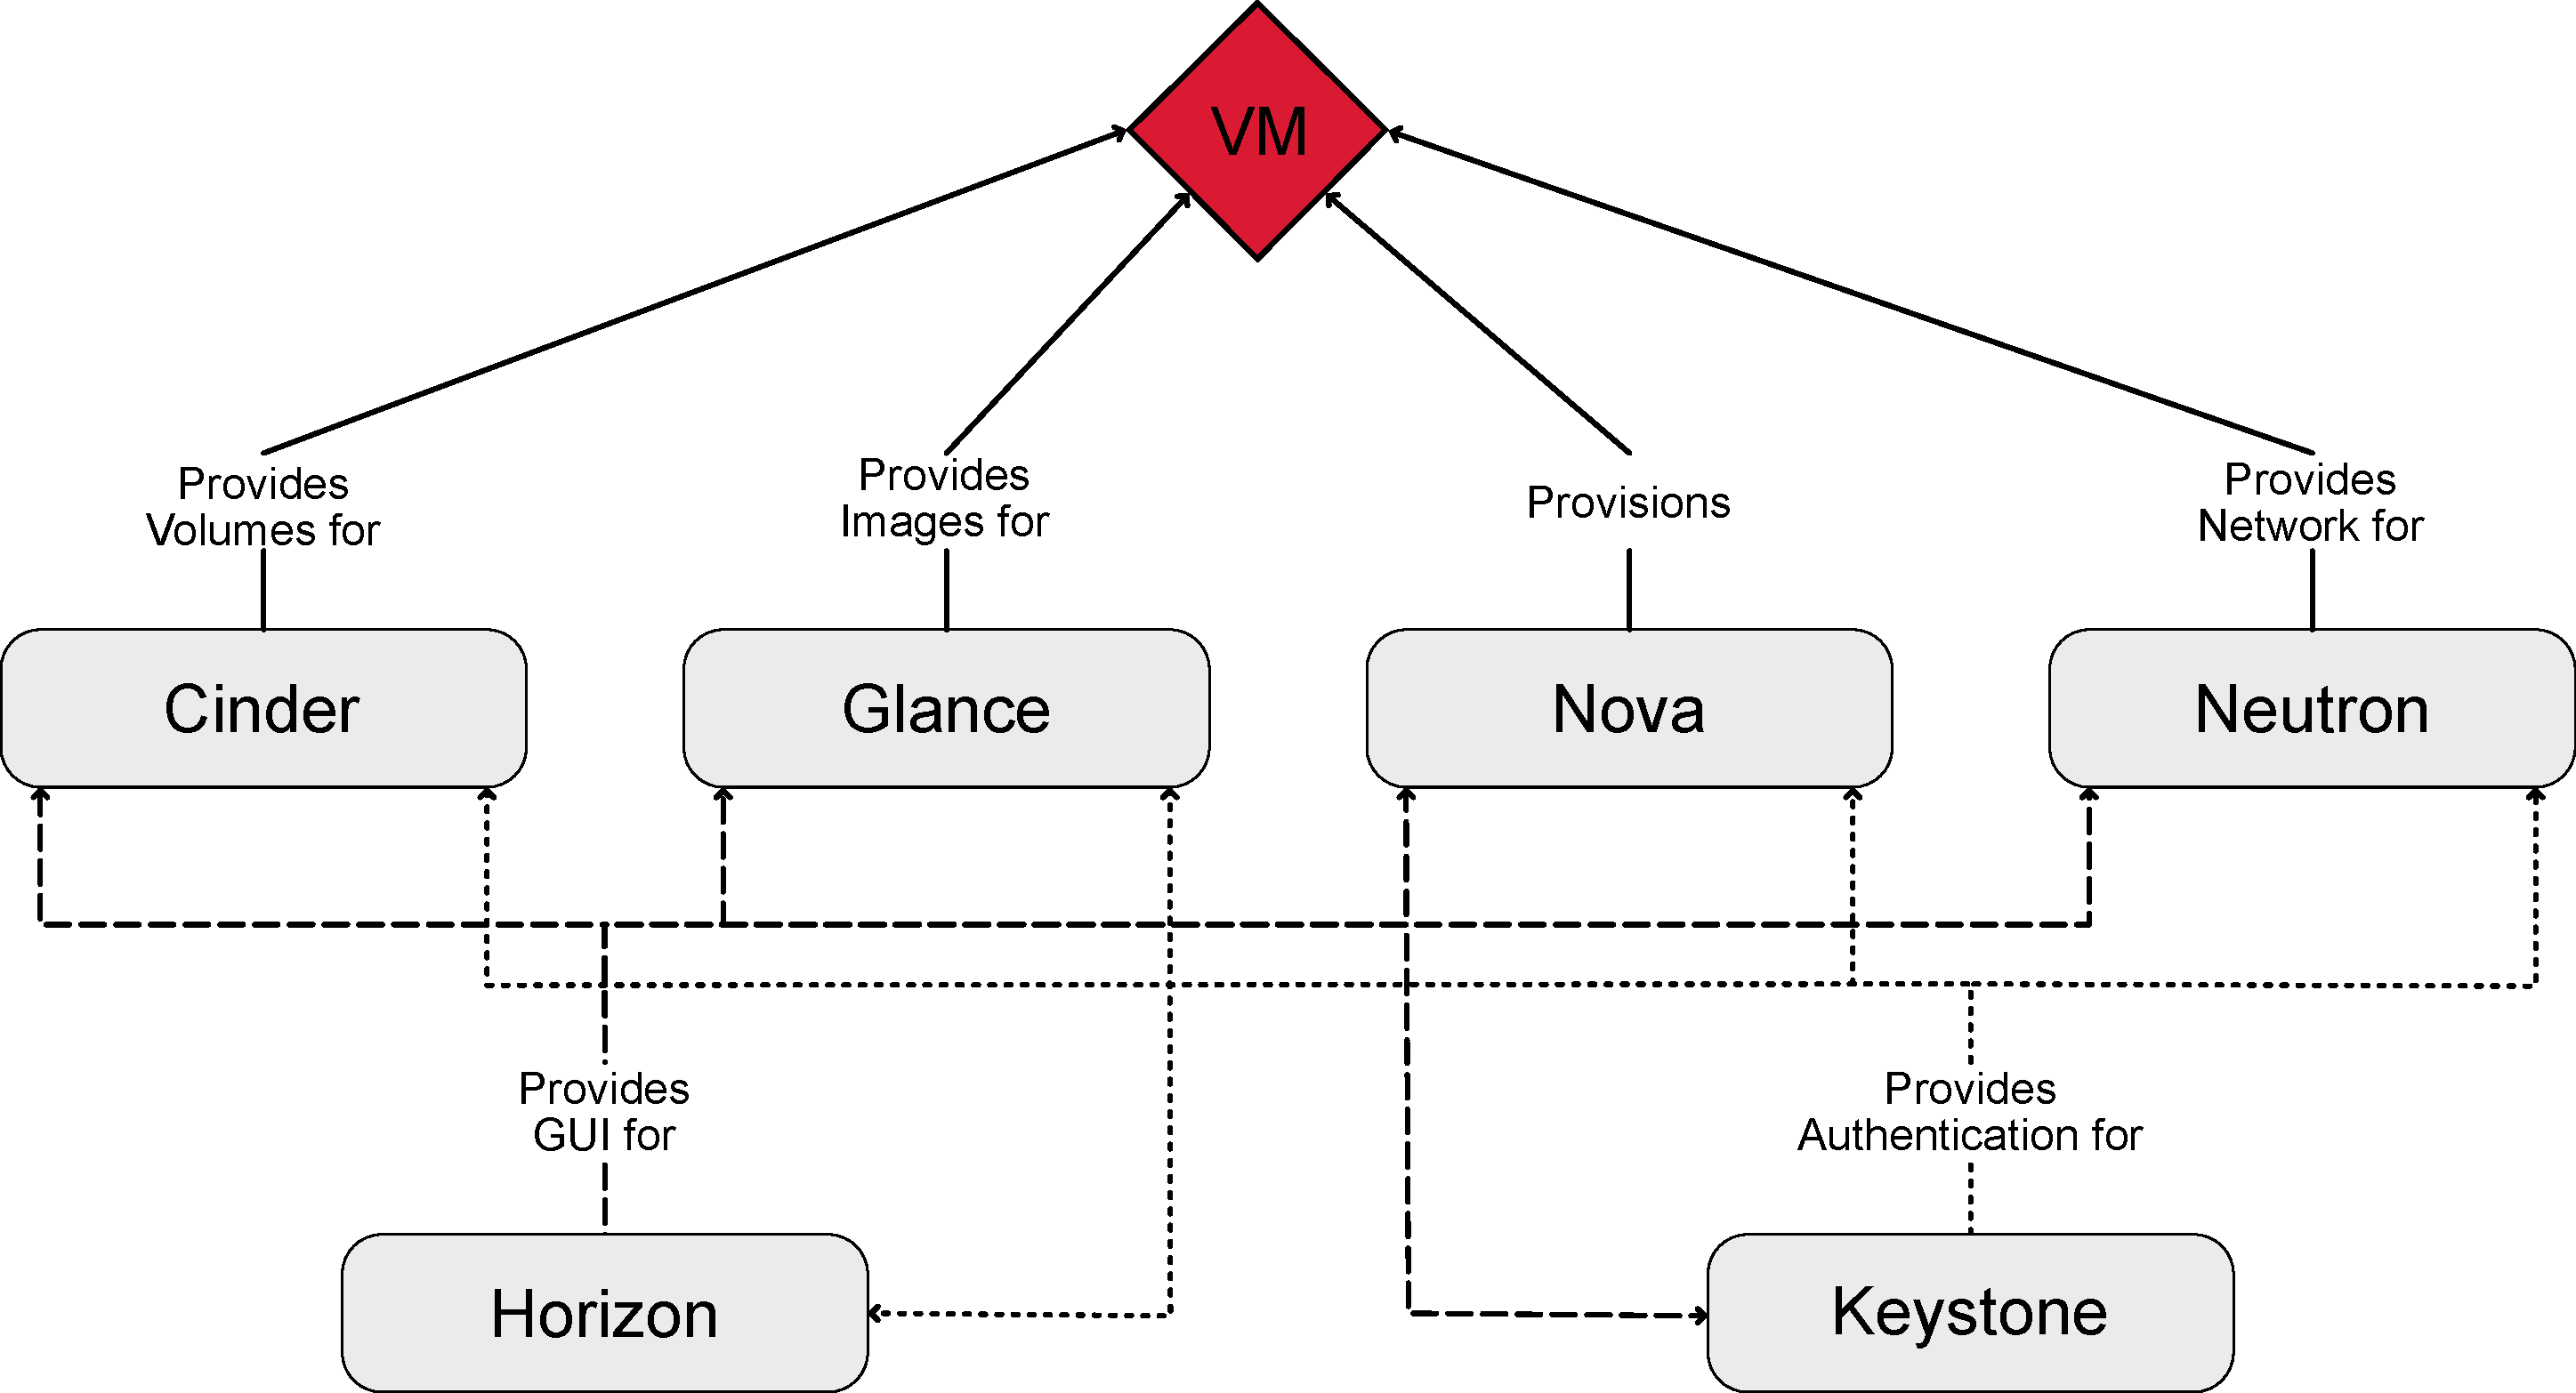
\includegraphics[width=0.7\textwidth ]{02_openstack-components.pdf} 
                    \caption[Interaction of OpenStack components]{Interaction of OpenStack components \cite{UnixArena2015}}
                    \label{figure:openstack_components}
                \end{center}	
             \end{figure}
             
             
             \subsubsection{Shared Services}
             
                Regarding shared services, the identity service \textsl{Keystone} and \textsl{Glance} are critical to a functioning OpenStack cluster.
                
                \noindent \textsl{Keystone} provides authentication for clients in the OpenStack environment. 
                Clients hereby refer to other OpenStack components, which need to authenticate their operations, as well as to actual clients, authenticating themselves to access the OpenStack cluster.
                
                \noindent \textsl{Glance} provides the functionality of registering and retrieving images for \acp{VM}.
                The actual images can be stored in various locations, and using Glance's \ac{API}, image metadata and the actual retrieval of the image is possible.
                
                \noindent Although not essential, the placement services \textsl{Placement} provides the functionality of tracking cloud resources and their usage.
                Using an API, Placement helps other services to manage and allocate their resources accordingly, which is an important factor in this thesis’s context. 
             
             
             \subsubsection{Web Frontend}
                 
                Although not strictly necessary for a functioning OpenStack Cluster, it was decided to use the canonical web interface \textsl{Horizon}.
                While also in an automotive or embedded context, a web interface would not be used, for the research and development performed in this thesis, it considerably increases the usability of OpenStack. 
                 
                 
             \subsubsection{Computing Services}
                 
                The computing service \textsl{Nova} provides the provisioning of compute instances.
                Nova provisions instances via \acp{VM}.
                Throughout this thesis, only \acp{VM} will be used to provision and consume compute services.
                Nova consists of three core services being the \textsl{Nova-Conductor}, \textsl{Nova-Scheduler}, and \textsl{Nova-Compute}.\\
                Nova-Compute represents the resource provisioning.
                Its main objective is the communication with the hypervisor on the host and the \ac{VM}.\\
                The Nova-Scheduler is responsible for choosing appropriate computing hosts.
                Based on a broad space of parameters, the scheduler can be configured to distribute \acp{VM} based on specific rules to compute hosts.
                It first filters all eligible hosts for, for example, satisfying the required resources, and second determines the best host based on the mentioned parameters.
                Chapter \ref{chapter:usecases} will examine the Nova-Scheduler in greater detail.\\
                The Nova-Conductor handles all requests requiring cluster-wide coordination.
                Figure \ref{figure:nova_architecture} shows the Nova service and the external components it is dependent upon.
                 
                 \begin{figure}[ht]
                    \begin{center} 
                        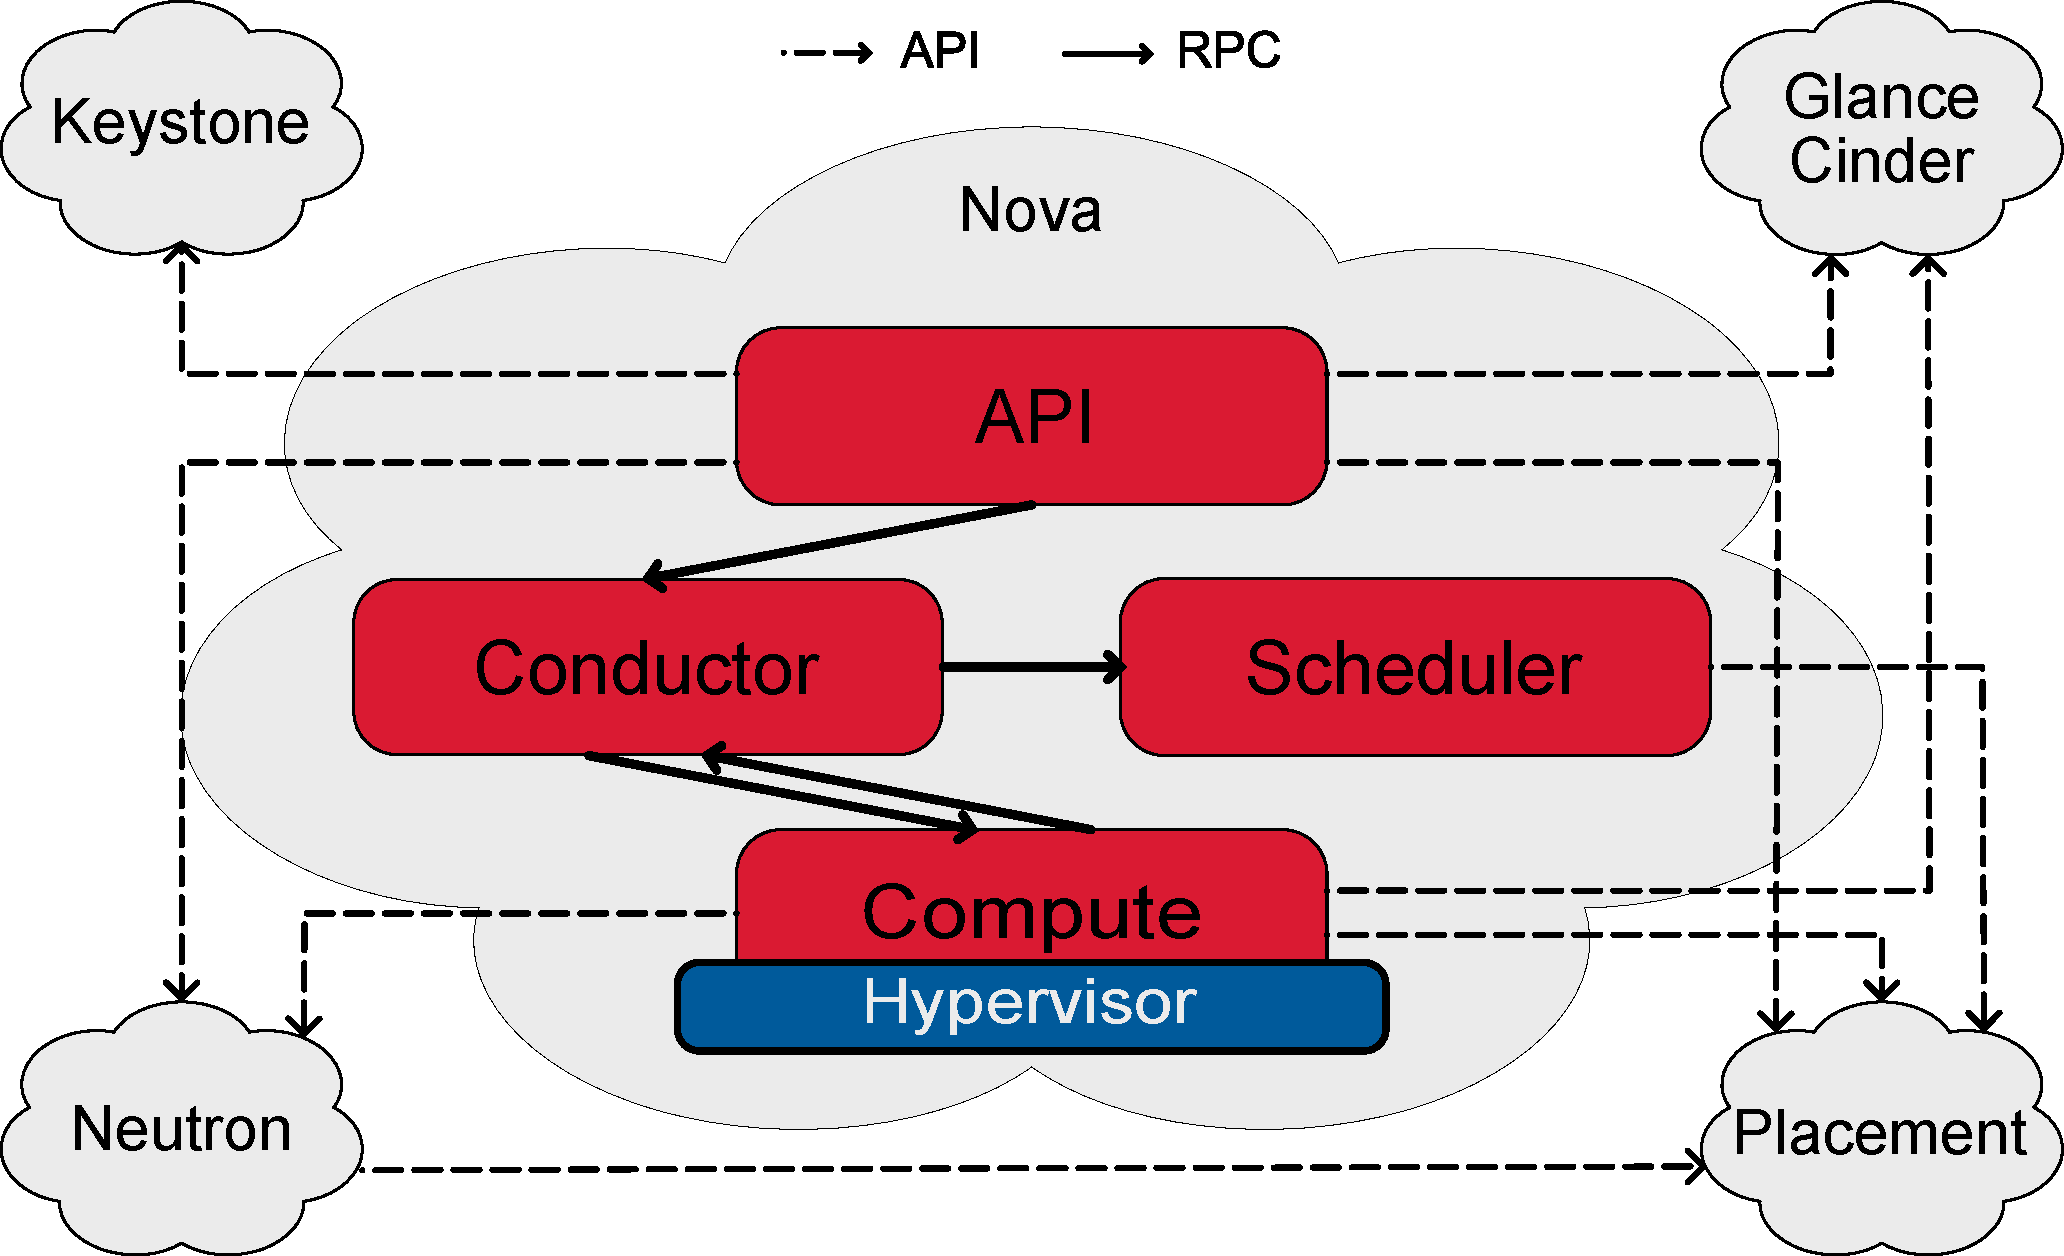
\includegraphics[width=0.7\textwidth ]{02_nova-architecture.pdf} 
                        \caption[OpenStack Nova architecture]{OpenStack Nova architecture \cite{OpenStackNSA2019}}
                        \label{figure:nova_architecture}
                    \end{center}	
                 \end{figure}
                 
                 
             \subsubsection{Networking Services}
             
                For the networking services, the OpenStack component \textsl{Neutron} is responsible.
                It focuses upon the delivery of Networking-as-a-Service to other OpenStack services, for example, to Nova-Compute instances.
                Neutron also supports creating multiple, on-demand networks along with all necessities like routers, switches, dynamic host configuration protocol, or domain name system services.
                 
                 
             \subsubsection{Storage Services}
                 
                OpenStack offers three different storage services.
                In this thesis, only the block-storage service \textsl{Cinder} will be considered.
                Cinder virtualizes and provides block-storage volumes to other components like Glance as well as for VMs themselves as storage.
                 

            
        \subsection{Communication Services}
            
            OpenStack communication mainly relies on two paradigms, which are used by all components and services.
            Following, \acp{API} and \acp{RPC} will be briefly described.
            
            \subsubsection{\acp{API}}
                
                All major OpenStack components contain an \ac{API} service.
                These \acp{API} expose one or more endpoints to the outside world to interact with.
                Other components and users themselves can use those endpoints to trigger actions or transfer data.
                The OpenStack command-line-tool and the Python \ac{SDK} make heavy use of the \ac{API} services to enable users to interact with OpenStack.
                
            
            \subsubsection{\acp{RPC}}
                
                Apart from \acp{API}, OpenStack heavily relies on \acp{RPC} for client-server intra-service communication. 
                For example, if the creation of a new \ac{VM} is requested, the Nova-Conductor (running on the controller) invokes Nova-Computer to build the \ac{VM} on a compute host via an \ac{RPC}.
                This is also indicated in Figure \ref{figure:nova_architecture}, where the communication inside the Nova component happens via \acp{RPC}, while the external communication happens via \acp{API}.
                The implementation of \acp{RPC} is achieved through the Advanced Message Queuing Protocol AMQP.
                All \acp{RPC} are packed into messages, which are then sent to a message broker, who further distributes the messages to the proper destinations.
                
\chapter{Host and Test Setup}
\label{chapter:host_and_Test_setup}

    To perform measurements and evaluate OpenStack, appropriate hardware is necessary.
    This hardware must also feature a certain OS, and the OpenStack components must be installed and configured.
    As embedded systems are not intended for Cloud Computing software like OpenStack, the installation and successful execution process includes difficulties.
    This chapter presents the hardware and software setup used for testing.
    
    
    \section{Hardware Setup}
    \label{section:hardware_setup}
        
        In order to study OpenStack on embedded systems, two different hardware platforms were chosen.
        To evaluate a broader spectrum of hardware, one platform was chosen to be x86-based, while the other was chosen to be an ARM-based platform.
        For the x86-based platform, an Intel Xeon Platinum \ac{CPU} with 24 cores was chosen.
        Due to having much computational power, systems based on this \ac{CPU} are currently used for developing autonomous driving.
        Therefore, this platform represents a powerful x86 embedded system intended for future use in automotive applications.
        The x86 platform comes further with 188 GB of memory and 960GB of NVMe secondary storage connected via a M.2 interface.\\
        A Renesas R-Car Starter Kit Pro, featuring a Renesas R-Car H3 SoC, was chosen for the ARM-based platform.
        With eight cores in a big.LITTLE architecture, this \ac{SoC} has four high-performance and four high-efficiency cores.
        It is specifically designed for the automotive industry and is currently used in automotive \acp{ECU}.
        The ARM platform comes with 4 GB of memory and a 64 GB SD-Card as secondary storage connected via an SD-Card interface.\\
        Table \ref{table:host_specs} shows the specifications of the hardware used.
        Both platforms are equipped with 1 Gbit network interfaces.
        The x86 platforms additionally come with a 10 Gbit network interface.

         \begin{table}[ht]
            \begin{center}
                \begin{tabular}{ c | c | c | c | c }
                    \textbf{Platform} 	& \textbf{Processor} 													& \textbf{Memory} 	& \textbf{Storage} 	& \textbf{Network} \\
                    \noalign{\hrule height 1.5pt}
                    x86			& \makecell[c]{Intel Xeon Platinum \\ 8160T @ 3.60 GHz (24 Cores)}				& 188 GB 			& 960 GB			& \makecell[c]{1x 1 Gbit \\ 1x 10 Gbit} \\[0.3cm]
                    ARM			& \makecell[c]{Renesas R-Car H3 \\ 4x Cortex-57 and 4x Cortex-53 } 			& 4 GB 			& 64 GB 			& 1x 1 Gbit
                \end{tabular}
            \caption{Hardware and specifications of the host systems used for testing}
            \label{table:host_specs}
            \end{center}        
        \end{table}
    
        \noindent Of each platform respectively, two systems were chosen to be used in the testing setup.
        As described in Section \ref{section:openstack}, an OpenStack cluster consists of different core services and additional separate components.
        Due to the high computational power and high memory, it was decided to configure one x86 platform as the controller node. 
        The other three nodes (2x ARM and 1x x86) were chosen to be configured as dedicated compute nodes.
        Figure \ref{figure:network_setup} shows the connection between all platforms, creating the OpenStack cluster.
        All platforms are connected via a Layer 2 1 Gbit Ethernet switch with Cat 5e Ethernet cables.
        However, the x86 platform configured as a compute node is in addition connected directly via a 10 Gbit Ethernet connection to the controller node.
        Further, the Ethernet switch is connected to a gateway via a 1 Gbit connection.
        The external network, though, is only used for installation and update purposes.
        
         \begin{figure}[ht]
             \begin{center} 
                    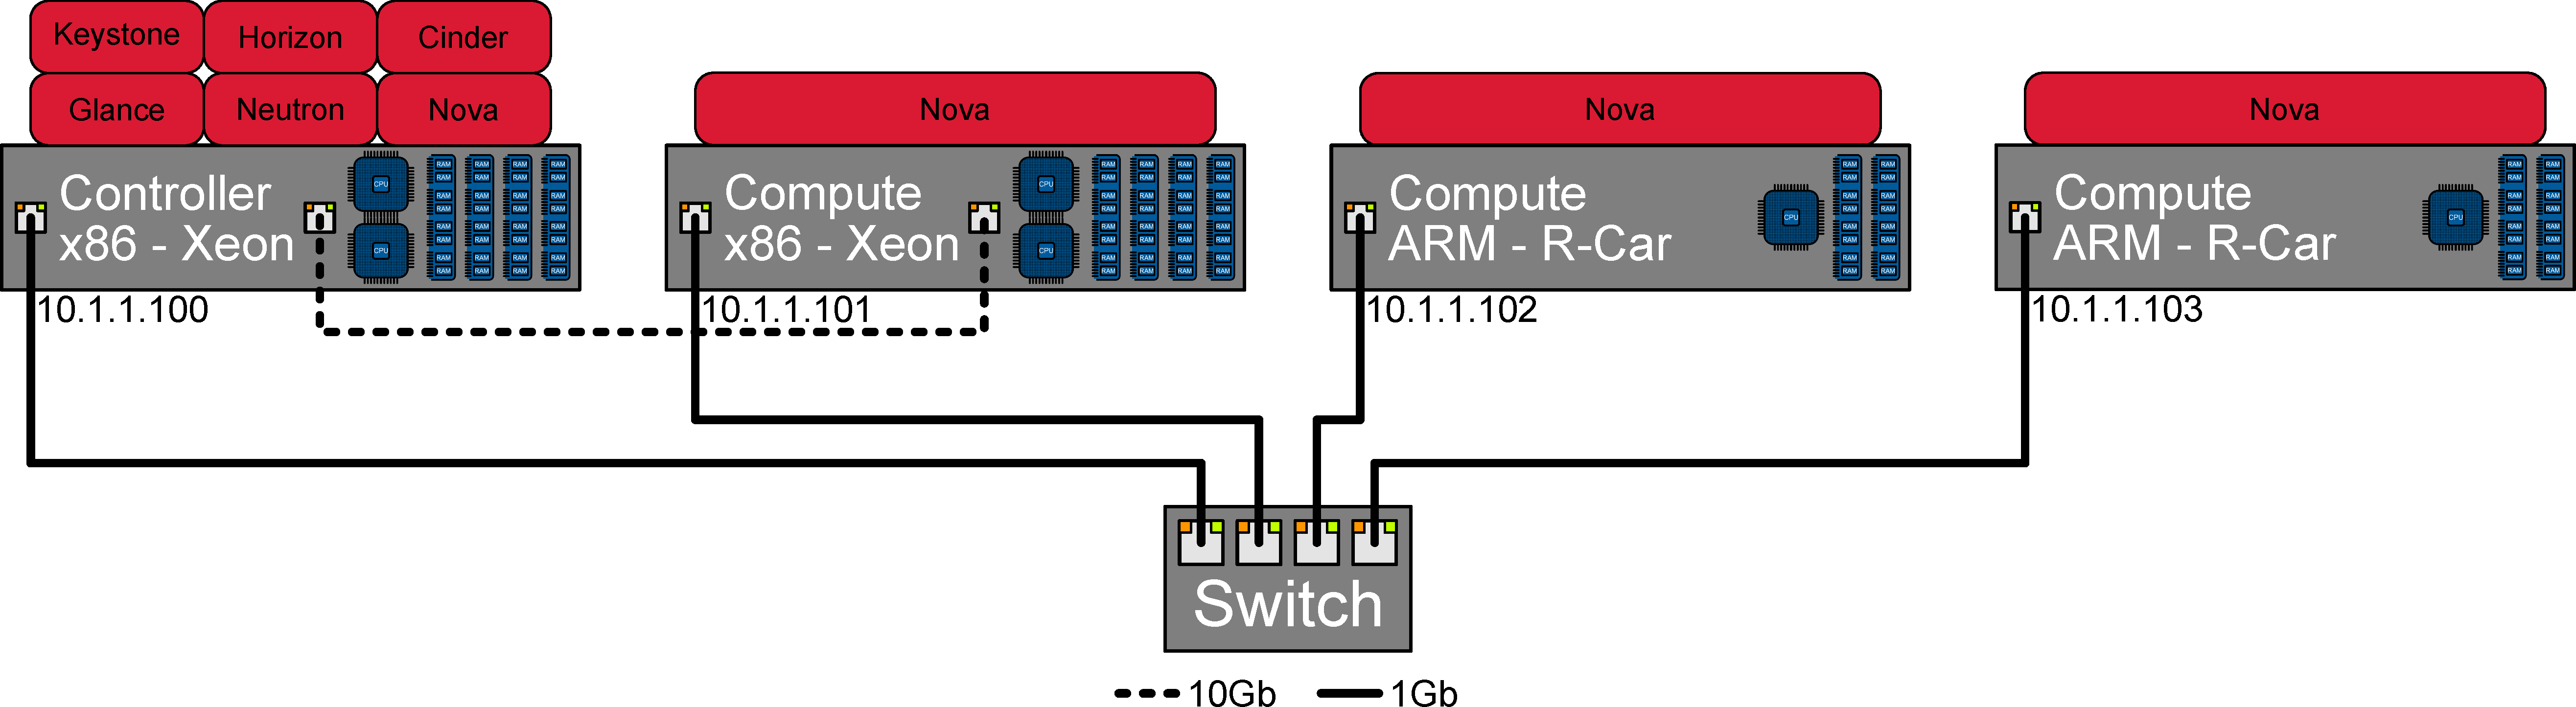
\includegraphics[width=\textwidth ]{03_network_setup.pdf} 
                    \caption{OpenStack hardware and network setup}
                    \label{figure:network_setup}
             \end{center}	
        \end{figure}
               
    
    \section{Software Installation}
    \label{section:software_installation}
        
        The installation process of all software consists of two stages.
        As a first step, the host system must be prepared.
        This preparation includes the OS, the correct configuration of necessary settings, and the installation of necessary packages and dependencies.
        As a second step, the OpenStack follows, including the installation and configuration of the OpenStack cluster.
        
        
        \subsection{Host System Preparation}
            
            Before installing the OpenStack services, the host systems must be prepared accordingly.
            For both platforms, Ubuntu 18.04 was chosen as the host \ac{OS} because of two reasons.
            First, Ubuntu is a Linux distribution supported and recommended by OpenStack, ensuring compatibility and better reliability with less unforeseeable complications.
            Second, using an Ubuntu distribution enables a simplified installation of OpenStack through DevStack\footnote{DevStack: https://docs.openstack.org/devstack/victoria/} and simplified interaction with the host system itself.
            For the x86 platform, an Ubuntu image already came prebuilt and preinstalled.
            Solely virtualization support had to be enabled in the BIOS settings.
            With the image being based on Ubuntu Server 18.04, a server \ac{OS} on primarily for server usage intended Intel Xeon \acp{CPU}, problems were neither anticipated nor encountered.
            
            \noindent Contrary to the Intel \acp{CPU}, the Renesas R-Car \acp{SoC} were neither intended to run Ubuntu as \ac{OS} nor OpenStack or similar software.
            This presents the first difficulty in integrating such \acp{SoC} as OpenStack nodes.
            The following paragraphs will briefly describe the problems and decisions made to prepare the \acp{SoC}.
            Table \ref{table:host_sw} shows the final \acp{OS} installed and the according kernel on each platform.
            
             \noindent \textbf{Installation of Ubuntu}
            Being an \ac{SoC} intended for embedded usage, the \ac{OS} usually is custom-built for the target system.
            Advantages of custom \acp{OS} lie in their small size by only including the necessary features, packages, and tools.
            To only include the necessary, all features and functionality in the form of packages must be known in advance.
            Together with a description of hardware features, a functional custom \ac{OS} can be created.
            As such image creation can be a tedious task, the Yocto Project was chosen for image creation.\\
            The Yocto Project\footnote{Yocto Project: https://www.yoctoproject.org} is an Open-Source project helping developers to create custom Linux-based systems \cite{Yocto2021}.
            Using the Yocto Project, packages needed in the image are specified through \textsl{recipes} and later \textsl{baked} into the final image.
            Similar, unique hardware properties are specified through the hardware manufacturer's board support packages and can be included in the image.\\
            Due to OpenStack's massive size, knowledge about all necessary packages and dependency in advance was impossible as this also includes all indirectly used libraries and packages.
            Although a particular repository exists, which aims at providing all recipes needed, tedious trials showed that the repository was not an option.
            Due to version constraints, the recipes for OpenStack were highly inconsistent, which hindered a successful image creation.\\
            For the final solution, it was decided to use a custom Yocto kernel along with a base version of Ubuntu.
            As Yocto generates all necessary outputs like kernel modules, they can be integrated and used by any \ac{OS}.
            To perform a successful installation of Ubuntu, the guide from \cite{Tnx942412020} was used and adapted accordingly.
            Summarized, both \acp{OS}, the Yocto generated and the Ubuntu one, were installed on separate partitions of an SD-Card.
            The Ubuntu OS was then configured to use the Yocto generated kernel and kernel modules.
            Although not having included the OpenStack packages into the image, the Ubuntu user space and especially aptitude enabled the standard way of installing any packages and other software.
            
             \noindent \textbf{Kernel Configuration}
            Using the described method to install Ubuntu relies on the kernel and the kernel modules built with the Yocto Project.
            As previously said, custom \acp{OS} contain only a minimal set of features and packages.
            The same applies to the kernel build with Yocto.
            Since OpenStack relies on many packages, which again rely on specific kernel modules, these kernel modules must be added explicitly to the kernel configuration in advance.
            By creating a kernel configuration file containing all necessary kernel modules and features, the Yocto build system can read which features and modules should be incorporated into the kernel.\\
            In addition to the basic Yocto kernel configuration, a few kernel modules have to be added.
            As OpenStack relies on network-based communication, \textsl{ebtables} and \textsl{netfilter} modules needed to be included.
            These modules enable the Linux firewall and packet filtering, which are substantial for OpenStack's internal communication.
            Further, \textsl{pseudo-filesystems} and \textsl{virtualization} had to be included.
            Pseudo-filesystems are necessary for OpenStack to keep track of the host systems' specific values and properties, while virtualization is necessary to virtualize resources.
            Last, the \textsl{device-mapper} module was necessary for OpenStack to manage storage as logical volumes for virtual machines.
            
             \noindent \textbf{Arm Trusted Firmware}
            As the last step in preparing the SoC the \ac{ATF} had to be reconfigured.
            The \ac{ATF} is a secure world software, that provides a trusted execution environment on a very low level \cite{Arm2021}.
            The crucial aspect of the \ac{ATF} for this thesis is that it must allow virtualization. 
            Otherwise, despite the kernel support, no virtualization of hardware resources is possible.
            In order to achieve this, individual files with specific configurations need to be generated. 
            Fortunately, Yocto also generates them automatically.
            Configuring the corresponding recipes to allow virtualization generates the according files.
            These files must then be flashed onto the \ac{SoC}.
            
            \begin{table}[ht]
            \centering
                    \begin{tabular}{ c | c | c }
                        \textbf{Platform} & \textbf{Kernel} 				& \textbf{OS} \\
                        \noalign{\hrule height 1.5pt}
                        x86			& 5.0.0-23-generic (x86\_64) 		& Ubuntu Server 18.04 \\
                        ARM			& 5.4.0-yocto-preempt-rt (aarch64)	& Ubuntu Base 18.04 
                    \end{tabular}
                \caption{Software specifications used on host systems for testing}
                \label{table:host_sw}   
            \end{table}
            
            
            
        \subsection{OpenStack Installation}
        \label{subsection:openstack_installation}
            
            Installing and configuring OpenStack can be a complicated, time-consuming, and error-prone task.
            Therefore, the DevStack scripts were chosen to install a complete OpenStack environment.
            OpenStack itself uses DevStack as a development environment and for functional testing.
            The future environment's configuration is made through a \textsl{local.conf} file, where parameters, settings, and services can be specified.
            In the following paragraphs, the configuration of the OpenStack cluster will be described and explained.
            
             \noindent \textbf{Installation}
            The DevStack documentation includes multiple different guides for installing an OpenStack environment.
            For the test scenarios and this thesis's scope, a multi-node environment was desired, with the main focus on compute services.
            Therefore, a minimal OpenStack configuration consisting of the services presented in Section \ref{subsection:components} was installed using the guide from \cite{OpenStackMNL2020}.
            Apart from Horizon, all services used represent the minimal set of services for an OpenStack environment.
            Horizon was also included for easier interaction with OpenStack and better visualization of current activities.
            As mentioned in Section \ref{section:hardware_setup}, an Intel Xeon node was chosen as the controller node due to its high computational power.
            All necessary core services were decided to be installed on this node, along with the compute services.
            This configuration makes the controller node also an all-in-one node.
            Evaluating the R-Car \acp{SoC} as a separate or additional controller node was not possible due to limited resources on the R-Car, especially the low memory.\\
            For the other nodes, only compute services and communication software was decided to be installed.
            The compute nodes were configured to communicate with the controller node if other services like network or storage services were needed.
            Due to later test purposes, a connection to the \acp{VM} was necessary, and the standard network configuration was not suitable.
            As OpenStack establishes a new internal network, there is no access from the external network possible.
            To make this possible, the OpenStack network's external interface needs to be connected to an actual physical interface.
            This can be achieved by specifying a public interface in the \textsl{local.conf} file, together with an exactly matching network configuration of the external network.
            Listings \ref{listing:local_conf_controller} and \ref{listing:local_conf_compute} show the final configuration files, which were used to install OpenStack.
                        
            \begin{listing}[htp]
                 \inputminted[frame=single, linenos, breaklines]{sh}{measurements/00_install-execute/03_local-conf-controller.sh}
                \caption{OpenStack controller node configuration file}
                \label{listing:local_conf_controller}
            \end{listing}
            
            \begin{listing}[htp]
                 \inputminted[frame=single, linenos, breaklines]{sh}{measurements/00_install-execute/03_local-conf-compute.sh}
                \caption{OpenStack compute node configuration file}
                \label{listing:local_conf_compute}
            \end{listing}

            \newpage
             \noindent \textbf{Post Installation Configuration}
            After installing OpenStack, all services were configured with default settings and standard configurations. 
            Although most of them were suitable and need not be changed, a few needed to be adjusted.
            The main configuration to adjust were the preconfigured flavors and images.
            DevStack automatically downloads and configures a Cirros x86 image for testing purposes.
            However, to mimic the host systems in the best way possible, Ubuntu 18.04 Cloud Images were chosen as guest images.
            Due to operating with two different \ac{CPU} architectures, one image for the x86 and one for the ARM-based platform was necessary.
            Both could be configured and uploaded to the Glance image service either via the command-line or the web interface.\\
            Next, DevStack also configures a couple of default flavors.
            A flavor in the context of OpenStack and overall Cloud Computing refers to the resource configuration of a \acp{VM}.
            Due to the intended testing of specific hardware in specific configurations, custom flavors had to be defined.
            Table \ref{table:flavors} lists all created and used flavors throughout this thesis.
            Distinct flavors were defined for each platform, as both platforms differ in performance capabilities.
            For each platform, one \textsl{max}-flavor was defined, representing the highest possible \ac{VM} configuration.
            The other flavors were derived from the minimal configuration on the ARM platform.
            Having to create \acp{VM} with at least one \ac{vCPU}, this corresponds to one-eighth of the host's \ac{CPU} resources on the ARM platform.
            Therefore, it was decided to create one flavor corresponding to one-eighth of all host's resources.
            The remaining flavors were derived by doubling the number of \acp{vCPU}, memory, and storage.\\
            Additional to the difference in \ac{CPU} architecture, the ARM platform further features a big.LITTLE architecture, consisting of four high-performance and four high-efficiency cores.
            At the time of writing this thesis, the KVM hypervisor cannot virtualize two different physical vCPUs simultaneously for one VM \cite{RussianNeuroMancer2019}.
            Trying to use high-efficiency and high-performance cores simultaneously results in an error of \ac{KVM}.
            To avoid \ac{KVM} choosing performance and efficiency cores simultaneously for one \ac{VM}, the flavors were configured to always and only use the performance cores.
            Therefore, the maximum number of virtualizable cores on the ARM hosts is reduced to four instead of eight.
             
            \noindent Finally, to access the \acp{VM} after creation, two additional settings needed to be changed.
            OpenStack, or rather Neutron, manages the traffic to the \acp{VM} using security rules.
            Based on these rules, only explicitly allowed traffic is forwarded from and to the \acp{VM}.
            In order to verify the connectivity of \acp{VM}, the internet control message protocol ICMP has to be allowed so that ping requests could reach the \acp{VM}.
            To further be able to log into the VM, \ac{SSH} connections had to be allowed.
            As Ubuntu Cloud Images disable password authentication via \ac{SSH} by default, authentication had to be performed using public and private key pairs.
            Ubuntu's Cloud Images use the cloud-init package\footnote{Cloud-Init Package: https://cloud-init.io} to retrieve additional information at the first boot from specific files or servers.
            OpenStack through Neutron provides a metadata service, which among others, can insert a specified public key into the \acp{VM} to enable a password-less \ac{SSH} authentication.
            
            \begin{table}[ht]
            \centering
                    \begin{tabular}{l !{\vrule width 1.5pt}  c | c | c | c | c}
                        \textbf{Name}	& \textbf{\makecell{rcar-01-\\256-06}}	&  \textbf{\makecell{rcar-02-\\256-06}	}	& \textbf{\makecell{rcar-01-\\512-06}}	& \textbf{\makecell{rcar-01-\\256-12}}	& \textbf{\makecell{rcar-max}}\\
                        \noalign{\hrule height 1.5pt}
                        \textbf{vCPUs}	& 1								& 2								& 1								& 1								& 4\\
                        \textbf{Memory}	& 256							& 256							& 512							& 256							& 2048\\
                        \textbf{Disk}	& 6								& 6								& 6								& 12								& 55\\
                        \multicolumn{1}{c}{}	& \multicolumn{1}{c}{}	& \multicolumn{1}{c}{}	& \multicolumn{1}{c}{}	& \multicolumn{1}{c}{}	& \multicolumn{1}{c}{}\\
                        \textbf{Name}	& \textbf{\makecell{xeon-06-\\21504-106}}	& \textbf{\makecell{xeon-12-\\21504-106}}	& \textbf{\makecell{xeon-06-\\43008-106}}	& \textbf{\makecell{xeon-06-\\21504-212}}	& \textbf{\makecell{xeon-max}}\\
                        \noalign{\hrule height 1.5pt}
                        \textbf{vCPUs}	& 6								& 12								& 6								& 6								& 48\\
                        \textbf{Memory}	& 21504							& 21504							& 43008							& 21504							& 174080\\
                        \textbf{Disk}	& 106							& 106							& 106							& 212							& 850\\
                    \end{tabular}
                \caption{OpenStack VM flavors}
                \label{table:flavors}
            \end{table}
            
            
            
            

            
            
            
    
    
    
    
    
    
    
    
    
    




\chapter{Test Methodology}
\label{chapter:methodology}

    To examine and answer the research question, several different tests and measurements are performed.
    According to the research question, it was decided to perform measurements to gather insights on two topics.
    First, as resources in the embedded automotive environment are restricted, OpenStack's introduced overhead has to be assessed.
    Second, the performance of relevant resources should not be impacted too much, otherwise, OpenStack would not bring any additional value.
    
    \noindent All measurements were decided to be performed using micro-benchmarks and Linux command-line utilities.
    The \textsl{Phoronix-Test-Suite}\footnote{Phoronix Test Suite: https://www.phoronix-test-suite.com}, together with the utilities \textsl{ping} and \textsl{sysstat}\footnote{Sysstat Benchmark: https://github.com/sysstat/sysstat}, were chosen to be used.
    As the measurements aim to observe OpenStack’s impact, two measurements are obtained for each host configuration. 
    The first measurement is performed on the freshly installed hardware natively, without any OpenStack services.
    The second measurement is performed inside an OpenStack \ac{VM} running on the same host.
    The percentage overhead is calculated according to Equation \ref{equ:overhead}.
    However, both, the percentage overhead and the absolute difference between the native and VM values are considered.
    
    \begin{equation}
    \label{equ:overhead}
        \text{Overhead} = \abs{1 - \frac{\text{VM Performance}}{\text{Native Performance}}}
    \end{equation}
    
    \noindent To achieve the best comparability between native and VM values, the \acp{VM} are configured in a way to match the host's system configuration as much as possible.
    This is achieved using the according \textsl{max}-flavor.
    Table \ref{table:machine_configs} shows the native and the \ac{VM} resources used.
    The R-Car \ac{VM} uses only four cores due to \ac{KVM}'s limitations, as explained in Section \ref{subsection:openstack_installation}.
    The chosen configuration of the \textsl{max}-flavor, although slightly lower than the native one, was found to function the most reliable.
    Additionally, Listing \ref{listing:install_tests} shows the commands to obtain and install all necessary tools and utilities for testing.
    
    \begin{table}[ht]
        \begin{center}
            \begin{tabular}{c|c|c}
                \textbf{Resource} 	& \textbf{Renesas R-Car} 	& \textbf{Intel Xeon} \\
                \noalign{\hrule height 1.5pt}
                \begin{tabular}{c} \\ CPU \\Disk \\ Memory \end{tabular} 
                &
                \begin{tabular}{c|c} 
                    native & virtual \\
                    \noalign{\hrule height 1pt}
                    8 cores & 4 cores \\
                    59GB & 55GB \\
                    2GB & 4GB
                \end{tabular}
                &
                \begin{tabular}{c|c} 
                    native & virtual \\
                    \noalign{\hrule height 1pt}
                    48 cores & 48 cores \\
                    980GB & 850GB \\
                    188GB & 170GB
                \end{tabular}
            \end{tabular}
        \caption{Configuration of native and virtual machines for overhead measurements}
        \label{table:machine_configs}
        \end{center}        
    \end{table}
    
    \begin{listing}[ht]
         \inputminted[frame=single, linenos, breaklines]{bash}{measurements/00_install-execute/04_install.sh}
        \caption{Linux commands for installing all test utilities}
        \label{listing:install_tests}
    \end{listing}
      
    %----------------------------------------------------------------------------------------
    % Idle Usage
    %----------------------------------------------------------------------------------------
    \section{Idle Resource Consumption}
    \label{section:methodology_idle}
   
        OpenStack naturally introduces an unavoidable overhead.
        First, OpenStack's fundamental overhead introduced to the \ac{CPU} and memory is considered.
        While providing the OpenStack functionality, several additional processes are running.
        Consuming resources like \ac{CPU} and memory, if the idle overhead of the OpenStack services is too high, OpenStack would be unreasonable on such hardware.
        
        \noindent The hereby measured values are the \ac{CPU} and memory usage.
        As a baseline measurement, the system's \ac{CPU} and memory usage is measured and recorded every 5 seconds for a total of 500 seconds.
        The CPU usage values are gathered using the command ”sar 1 5”, which returns the average CPU usage during 5 seconds in percent, measured every second. 
        The memory usage is gathered from the \textsl{meminfo}-file in the \textsl{/proc}-directory.
        Containing the total memory value \textsl{MemTotal} and the currently free memory value \textsl{FreeMem}, the currently used memory can be calculated.\\
        For comparison, the OpenStack services are installed, and the same measurements are repeated with a minor adjustment.
        In advance, a \ac{VM} is created on the system under test and switched off.
        The measurements are taken in the same manner, except that after 200 seconds, the \ac{VM} is started.
        These measurements first enable gathering insights on the overhead of OpenStack’s services when running in an idle state. 
        Secondly, insights on the overhead during a VM's startup and its provisioning in an idle state without any load are gathered.
        Listing \ref{listing:idle_test} shows the bash-script used to gather the information with running OpenStack services.
        For gathering the baseline values, the same script without lines 8-11 is used.

        \begin{listing}[ht]
            \inputminted[frame=single, linenos, breaklines]{bash}{measurements/00_install-execute/04_startup.sh}
            \caption{Bash-Script for gathering CPU and memory usage values}
            \label{listing:idle_test}
        \end{listing}

    
    \section{Resource Performance Measurements}
    \label{subsection:methodology_impact}
        
        To further determine whether OpenStack's overhead is substantial or not, the impact on four core resources is examined.   
        Relevant resources in the context of embedded systems and Cloud Computing are the \ac{CPU}, memory, storage, and the network \cite{Gillam2013,Kominos2017,Kang2017,Vedam2012,Tesfatsion2018}.
       
        %----------------------------------------------------------------------------------------
        %	CPU Performance
        %----------------------------------------------------------------------------------------
        \subsection{CPU Performance}
        \label{subsection:methodology_cpu}
        
            While gaining advantages through \acp{VM}, as little as possible computational performance should be sacrificed.
            Through virtualizing the \ac{CPU} although, a particular overhead is introduced.
            Depending on the application, instructions from the \ac{VM} have to be processed first by the hypervisor, and only then can they be executed on the hardware.
            The performance impact must not be high, otherwise, computations inside \acp{VM} would not be realizable or require enormous host resources.
            
            \noindent To measure the \ac{CPU} overhead, a compilation of the Linux kernel is performed, and the time needed is used as a performance indicator.
            The benchmark \textsl{Timed Linux Kernel Compilation}\footnote{Timed Linux Kernel Compilation Benchmark: https://openbenchmarking.org/test/pts/build-linux-kernel} from the Phoronix-Test-Suite is used to perform this measurement.
            Listing \ref{listing:cpu_test} shows the command to execute the test.
            The compilations' speed can be significantly increased by using multiple threads, for example, using one thread per core.
            This makes the test also suitable to examine multicore performance and parallel workloads.
            
            \noindent To evaluate the platform as good as possible, the following decisions were made regarding the \ac{vCPU} configuration.
            Having 24 identical cores with hyper-threading, the Intel Xeon CPU is perceived as a 48 core \ac{CPU}.
            The cores' equality enables \ac{KVM} to also manage VMs with up to 48 \acp{vCPU}, which was chosen for the test VM on the x86 platform. \\
            The Renesas R-Car \ac{SoC} being an ARM SoC with big.LITTLE architecture consists of eight cores.
            Due to \acp{KVM} limitation to only virtualize the same types of cores simultaneously, the highest number of \acp{vCPU} for a virtual machine is reduced to four cores.
            Therefore, the native compilation on the R-Car is also performed using four threads instead of eight to achieve comparable results.
            Using the same number of threads as CPU cores, the CPU is utilized to 100\%, creating a maximum stress scenario.            
            
            \begin{listing}[ht]
                \inputminted[frame=single, linenos, breaklines]{bash}{measurements/00_install-execute/04_cpu.sh}
                \caption{Command for executing the CPU performance test}
                \label{listing:cpu_test}
            \end{listing}


        %----------------------------------------------------------------------------------------
        %	Storage Performance
        %----------------------------------------------------------------------------------------
        \subsection{Secondary Storage Performance}
        \label{subsection:methodology_storage}
            
            As storage and retrieval of data become more important, the secondary storage performance must not be a bottleneck.
            Again, through OpenStack as an additional middleware layer between the application inside a \ac{VM}, and the actual storage device, data must pass through more instances, which affects performance.
            This could throttle the computation by the \ac{CPU} or even prevent any computations in reasonable time frames. 
            
            \noindent Performance in the area of storage can be defined by the throughput parameter.
            The term throughput describes the amount of data that can be written or read from storage in a specific amount of time, for example, per second.
            While storage performance should not correlate to the storage's actual size, the \ac{VM} storage was nevertheless chosen to be as close to the original size as possible.
            For measuring the throughput, the \textsl{FIO} benchmark\footnote{FIO Benchmark: https://git.kernel.dk/cgit/fio/} of the Phoronix-Test-Suite was chosen because of its high configurability and recommendation \cite{OpenStackHTG2016}.
            To evaluate the available storage speed, values for sequential read and write operations are measured, as these reflect the most common operations.
            Listing \ref{listing:disk_test} shows the command for the test execution, which is performed on all systems without buffering and using the direct mode to avoid caching effects.
            
            \begin{listing}[ht]
                \inputminted[frame=single, linenos, breaklines]{bash}{measurements/00_install-execute/04_disk.sh}
                \caption{Command for executing the storage performance test}
                \label{listing:disk_test}
            \end{listing}


        %----------------------------------------------------------------------------------------
        %	Memory Performance
        %----------------------------------------------------------------------------------------
        \subsection{Memory Performance}
        \label{subsection:methodology_memory}
        
            Today's application execution takes mainly place from memory.
            Therefore, memory performance contributes a major part to the computational performance of a system.
            Similarly to the processor, as little as possible, performance sacrifices are desired, so OpenStack's impact on the memory should especially be as low as possible.
            
            \noindent For evaluating the memory's performance, again, the throughput of the memory can be considered.
            Depending on the memory's throughput, more or fewer operations are possible, and more or fewer data can be processed.
            To measure the memory's throughput, the \textsl{Stream} benchmark\footnote{Stream Benchmark: http://www.cs.virginia.edu/stream/} \cite{McCalpin1995} from the Phoronix-Test-Suite is used.
            This benchmark was also chosen because of its recommendations \cite{OpenStackHTG2016}.
            Table \ref{table:stream_kernels} shows the operations performed by the benchmark to measure the memory's throughput.
            Although the test also evaluates the throughput of a memory copy operation, this operation is not considered in this thesis for two reasons.
            First, memory copy operations are less common in embedded programming and embedded applications because of memory wastage.
            The usage of pointers and value passing by reference is more common and preferred so that zero-copy memory can be achieved.
            Second, the computational performance is more in focus, which is represented by the chosen operations.
            Like the kernel compilation, this benchmark also uses multiple cores and executes one thread per core by default.
            As described previously, being able to equip the R-Car \ac{VM} with only four cores, the benchmark is natively also executed using only four instead of eight threads.
            Listing \ref{listing:memory_test} shows the according command to execute the test.
            Additionally, the \acp{VM} memory was chosen not to be 100\% of the native hardware but a bit less.
            This should prevent the \ac{VM}'s from being killed by the host system due to using too much memory when it should become rare.
            However, this should not impact the memory’s performance while enabling the host system to run with enough memory. 
            
            \begin{table}[ht]
                \begin{center}
                    \begin{tabular}{l|l}
                        \textbf{Kernel Name} & \textbf{Operation} \\
                        \noalign{\hrule height 1.5pt}
                        Copy 		& $a(i) = b(i)$ \\
                        Scale 	& $a(i) = q \cdot b(i )$\\
                        Add 		& $a(i) = b(i) + c(i)$
                    \end{tabular}
                \caption[Vector operations of the Stream memory benchmark]{Vector operations of the stream memory benchmark \cite{McCalpin1995}}
                \label{table:stream_kernels}
                \end{center}        
            \end{table}
            
             \begin{listing}[h]
                \inputminted[frame=single, linenos, breaklines]{bash}{measurements/00_install-execute/04_memory.sh}
                \caption{Command for executing the memory performance test}
                \label{listing:memory_test}
            \end{listing}

        %----------------------------------------------------------------------------------------
        %	Network Performance
        %----------------------------------------------------------------------------------------
        \subsection{Network Performance}
        
            Communication between different instances and \acp{ECU} takes place over the network, and therefore its performance as well must not be degraded too much.
            Performance in terms of networking can be defined by two values: throughput and latency.
            Throughput again refers to the amount of data that can be sent or received in a particular time interval.
            Latency, on the other hand, refers to the duration between the emit of a packet and its reception at the destination.
            All network tests are only performed inside the test network to receive reliable and uninfluenced results.
            
            \noindent To measure both values, two different tests are performed.
            For throughput measurement the \textsl{Netperf} benchmark\footnote{Netperf Benchmark: https://github.com/HewlettPackard/netperf} from the Phoronix-Test-Suite is used.
            This benchmark measures the throughput during a TCP file send and TCP stream between client and server and vice versa.
            For latency measurement, the standard Linux command-line utility \textsl{Ping} is used. 
            For 100 seconds, every second a ping is sent, and the average response time of all pings is considered.
            Both tests require a counterpart for the system under test to communicate with.
            Table \ref{table:network_counterparts} shows the systems under test and the hosts used as Netperf-Server and Ping-Partner.
            Listing \ref{listing:network_test} shows the commands for the network tests execution.
            
            \begin{table}[ht]
                \begin{center}
                    \begin{tabular}{l|l|l}
                        \textbf{System} 		& \textbf{Netperf-Server} 	& \textbf{Ping-Partner} \\
                        \noalign{\hrule height 1.5pt}
                        R-Car compute	&  Xeon compute	& Gateway, Xeon controller \\
                        Xeon compute 	&  Xeon compute	& Gateway, Xeon controller \\
                        Xeon 	controller 	&  Xeon controller	& Gateway, Xeon compute
                    \end{tabular}
                \caption{Network test hosts and their counterparts}
                \label{table:network_counterparts}
                \end{center}        
            \end{table}
            
             \begin{listing}[ht]
                \inputminted[frame=single, linenos, breaklines]{bash}{measurements/00_install-execute/04_network.sh}
                \caption{Commands for executing the network performance tests}
                \label{listing:network_test}
            \end{listing}

    
            
            
            
            
            
            
            
            
            
            
            
            
            
            
            
            
            
            
            
            
            
            
            
            
\chapter{Measurements}
\label{chapter:measurements}
    
    Executing the previously described tests, extensive results were gained on all tested platforms.
    The following chapter presents the results obtained.
    Apart from a description, causes for specific results are identified and their implications  discussed.

    
    \section{OpenStack's Resource Consumption}
    \label{section:evaluation_consumption}
    
        \begin{figure}[ht]
          \centering
          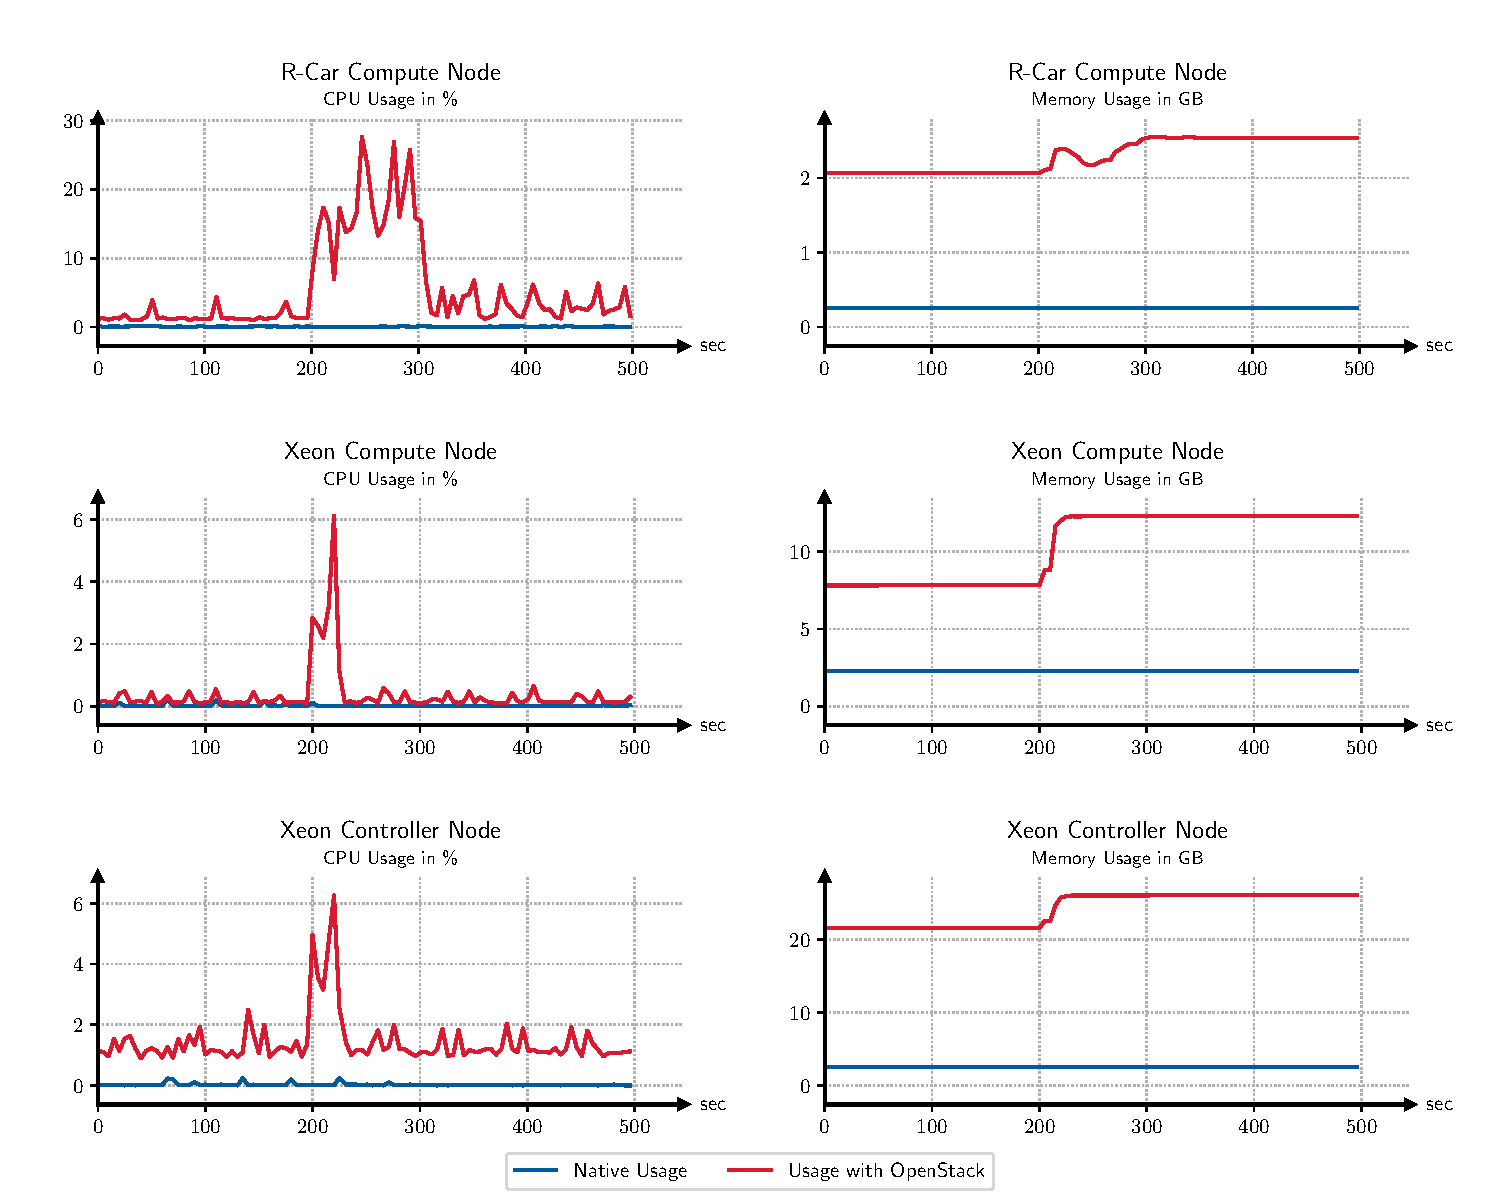
\includegraphics[width=\linewidth]{05_all-startup.pdf}
          \captionof{figure}{Idle CPU and memory usage on all tested platforms}
          \label{fig:all_idle}
        \end{figure}
        
        \newpage
        \noindent According to Section \ref{section:methodology_idle}, the CPU and memory usage is measured on a system with and without active OpenStack services.
        The goal is to examine the overhead introduced by solely running OpenStack services and provisioning one \ac{VM}.
        For all systems, a baseline measurement is performed to enable the comparison against the native system.
        Regarding the native CPU usage, all platforms have a nearly 0\% CPU usage due to being a fresh installation with no active services.
        As for the native memory usage, with 400 MB the R-Car node has clearly a smaller memory usage than the Xeon nodes. 
        This is expected because of the R-Car's custom kernel with an Ubuntu 18.04 Base \ac{OS}, contrary to the Xeon's full Ubuntu 18.04 Server \ac{OS} and standard Linux kernel.
        As expected, both Xeon nodes have similar memory usage of about 2.5 GB running without OpenStack.        
        
        \noindent Installing OpenStack on all R-Car and Xeon nodes (see Figure \ref{figure:network_setup}) indeed introduces overhead on the \ac{CPU} and memory.
        Clearly visible, the OpenStack services introduce on all platforms small periodic peaks.
        These are due to OpenStacks's periodic services, which poll information from all compute hosts.
        Starting the scenario described in Section \ref{section:methodology_idle}, the first 200 seconds in each plot in Figure \ref{fig:all_idle} show the resource usage for all services running in an idle state and a configured but turned-off VM.
        On the R-Car compute node, the \ac{CPU} usage increases by 2\% on average, while on the Xeon compute node, it increases by only 0.3\% compared to the native usage.
        This is due to the much higher core number and higher performance of the Xeon CPU, leading to an overall lower impact of the additional services. 
        On the other hand, on the Xeon controller node, the \ac{CPU} usage increases significantly by about 1\%.
        The significant increase compared to the Xeon compute node depicts the additional core services running the controller node.
        This threefold increase in CPU usage versus the Xeon compute node indicates that all controller services are about two times as heavy as the compute services.
        Continuing with the \ac{VM}'s startup after 200 seconds, it is visible that the R-Car requires much more \ac{CPU} power to perform the startup.
        Also, the longer-lasting \ac{CPU} usage increase shows that the startup takes about four times longer on the R-Car node than on the Xeon nodes.
        Compared to the scenario with a turned-off VM (first 200 seconds), an active but idle VM only impacts the \ac{CPU} usage on the R-Car node.
        After ca. 225 seconds on the Xeon nodes, the VM started successfully and runs in an idle state, introducing no visible overhead compared to a turned-off VM.
        After ca. 310 seconds, the VM also started successfully on the R-Car but influences the CPU more visibly compared to a turned-off VM.
        Again the lower impact on the Xeon nodes can be attributed to the overall higher performance of those CPUs and the therefore smaller impact of more load.
        
        \noindent Considering memory usage, similar observations can be made.
        Compared to an idle system, the OpenStack services and the turned-off VM introduce an overhead of 1.8 GB (2.0 GB total)  on the R-Car and about 5 GB (7.5 GB total) on the Xeon compute node.
        Further, on the Xeon controller node, OpenStack requires additional 19 GB of memory (21,5 GB total) to provide all core and compute services.
        Assuming the compute services behave similarly as on the Xeon compute node, all controller services require about 14 GB of additional memory, making them about three times as heavy as the compute services.
        However, these memory values are influenced by the yet turned-off \ac{VM}.
        Measuring the memory usage without any \ac{VM}, the R-Car shows a total memory usage of 900 MB, while the Xeon compute and controller nodes show a total usage of 3.1 GB and 13 GB.
        This corresponds to an overhead of about 400-500 MB on the compute nodes and about 13 GB on the controller node solely through the OpenStack services..
        Starting the \ac{VM} increases the memory usage on all platforms.
        An increase of about 400 MB is measured on the R-Car node, and the Xeon nodes require an additional 4 GB for the \ac{VM} provisioning. 
        Once the \ac{VM} is booted successfully, the memory usage does not change due to the \ac{VM} also being in an idle state without any running services inside.
        The higher memory required by the Xeon nodes correlates to the higher \ac{VM} memory configuration.
        Starting a VM with a lower memory configuration reduces this memory increase.
        
        \noindent Overall, the results confirm the introduction of overhead through OpenStack.
        However, an \ac{CPU} usage overhead of about 3-4\% on the R-Car nodes and especially of about 0.2\% on the Xeon compute node while provisioning \acp{VM} is lower than expected.
        An overhead in such dimensions does not rule OpenStack out on these systems.
        The same applies to memory usage. 
        Especially the lower memory usage on the R-Car nodes is interesting and suggests a more in-depth examination.
        The controller node requires more memory and more CPU performance due to the additional core services. 
        This advices to use a powerful enough system or dedicated network and storage nodes to provide the core services.
        The difference regarding both platforms' overhead originates from the high difference in computational performance and the chosen VM configurations.
        This makes the platforms not directly comparable but suggests considering them as possible low-end and high-end platforms.
        

    \section{OpenStack's Impact on Resources}
    \label{section:evaluation_performance}
        
        Examining the in Chapter \ref{chapter:methodology} defined resource's performance, the measurements show that all resources suffer some performance degradation.
        In all performed tests, the OpenStack \acp{VM} are outperformed by the native hardware.
        As expected, the R-Car node performs overall weaker than the Xeon nodes due to not being intended for such a use case and representing a low-end hardware.
        However, the impact on none resource is substantial enough to entirely exclude OpenStack on either the ARM or the x86 platform.
        The following sections present the measurements on every resource.
        
        \subsection{Effects on the CPU}
        \label{subsection:cpu_impact}
            
            \begin{figure}[ht]
              \centering
              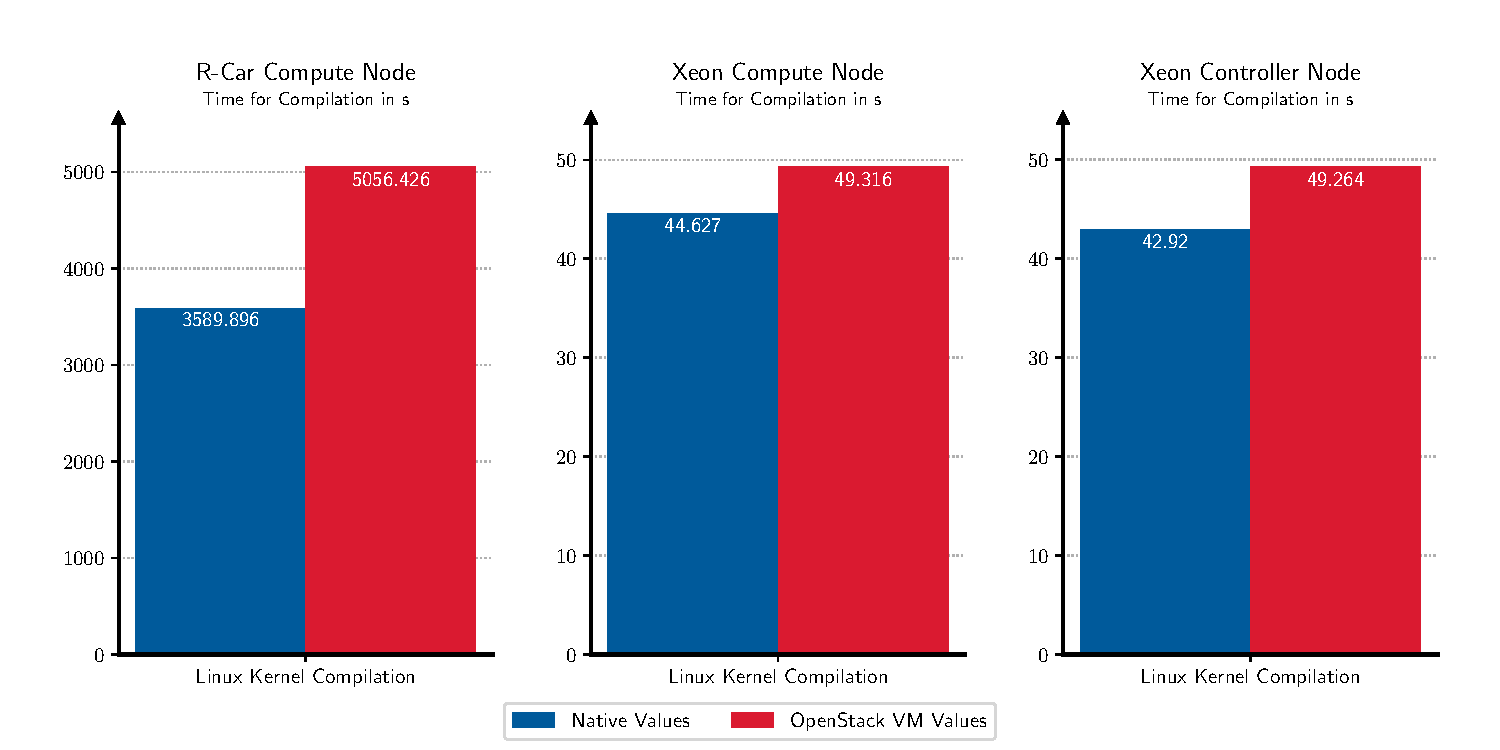
\includegraphics[width=\linewidth]{05_all-cpu.pdf}
              \captionof{figure}{Timed Linux Kernel compilation on all tested platforms}
              \label{fig:all_cpu}
            \end{figure}
            
            \noindent To evaluate the CPU performance degradation inside a VM, a Linux kernel compilation was chosen to stress the CPU, as explained in Section \ref{subsection:methodology_cpu}.
            Examining the difference in time between the native and the \ac{VM} compilation, a bigger difference is found on the R-Car node. 
            On the Xeon compute node, the \ac{VM} is about 4.7 seconds or 9.5\% slower, and on the Xeon controller node, it is about 6,3 seconds or 12.9\% slower.
            The weaker performance on the controller node is due to the additional services running and the, therefore, higher CPU load.
            Interestingly, both Xeon \acp{VM} perform nearly the same, with the difference being the native value, which is better on the controller node.
            However, a performance overhead of 10\% by the compute services on the compute node is tolerable.
            As the Xeon controller node in the here used configuration would represent the worst-case performance, an overhead of 13\% is also acceptable.
            
            \noindent The R-Car node, on the other hand, performs far worse.
            Comparing the \ac{VM} compilation versus the native compilation, the \ac{VM} takes about 1466 seconds or 29\% longer to compile the kernel.
            Introducing such performance degradation, OpenStack would not be usable on this hardware.
            The R-Car's high overhead is, on the one hand, due to the low core number and its big.LITTLE architecture, on the other hand, due to the R-Cars low secondary storage performance.
            As described in Chapter \ref{chapter:host_and_Test_setup}, the VM's cores are pinned to the host's high-performance cores.
            Through pinning the \acp{vCPU} to actual physical \ac{CPU} cores, the virtual processes are executed on predefined \acp{CPU} cores.
            Contrary to the Xeon nodes, this takes the ability to reschedule these tasks to other cores by the host \ac{OS}.
            Having enough cores to prevent a high utilization of one core, this should not impact the performance.
            However, the kernel compilation utilizes the full \ac{vCPU} and, therefore, all physical high-performance cores by 100\%.
            As the actual OpenStack compute services on the host also require computational power, they are simultaneously executed on the high-performance cores, leading to an over-utilization of those cores.
            This further leads to worse performance in general.
            Also, during the compilation process, many relatively small files need to be read from storage. 
            Due to the low secondary storage performance on the R-Car, found and discussed in Section \ref{subsection:disk_impact}, the results are further influenced and not 100\% representative.
            The R-Car results represent a worst-case scenario of a highly utilized CPU and low storage performance. 
                        
            \noindent Figures \ref{fig:two_threaded_host} and \ref{fig:two_threaded_vm} depict exemplary how a two-threaded instead of a four-threaded \ac{VM} task stresses the cores inside the \ac{VM} and on the actual host \ac{CPU}.
            Inside the VM, cores 1 and 2 are fully loaded, leading to also fully loaded cores 1 and 2 on the host itself.
            As only two threads are being used, cores 3 and 4 inside the VM are idle and barely used.
            However, despite the non-utilized VM cores, on the host the cores 3 and 4 show a usage of 20\% and 13\%, indicating that apart from the VM application OpenStack's compute services also require a certain amount of resources.
            
            \begin{figure}[ht]
            \centering
                \begin{subfigure}[b]{0.48\textwidth}
                    \centering
                    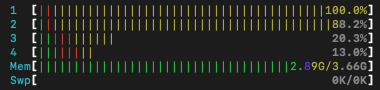
\includegraphics[width=\textwidth]{05_cpu-usage-rcar-compilation}
                    \caption{R-Car high performance cores utilization}
                    \label{fig:two_threaded_host}
                \end{subfigure}
                \hfill
                \begin{subfigure}[b]{0.48\textwidth}
                    \centering
                    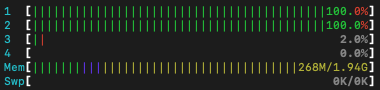
\includegraphics[width=\textwidth]{05_cpu-usage-vm-compilation}
                    \caption{VM cores utilization}
                    \label{fig:two_threaded_vm}
                \end{subfigure}
                \caption{Host and guest CPU utilization during a 2 threaded VM task}
                \label{fig:two_threaded_utilization}
            \end{figure}

            \noindent To gather better and more reliable insights, this test should be repeated first, on a broader range of hardware, and second, with a more precise configuration.
            The big.LITTLE architecture in this configuration of four high-efficiency and four high-performance cores is not ideal. 
            Through configuring, for example, the VM to used particular cores and the host to use other cores for the compute services, a mutual influence on each other could be prevented.
            Nevertheless, this would require hardware with sufficient computational power to provide sufficient resources to the host and the VM.
            Due to the over-utilization and deficient secondary storage performance, the results rather represent the worst-case. 
            However, through the better guest and host configuration regarding the utilized cores and better storage solutions, better and closer to reality results could be achieved.
           
        
        \subsection{Effects on the Secondary Storage}
        \label{subsection:disk_impact}
            
            \begin{figure}[ht]
              \centering
              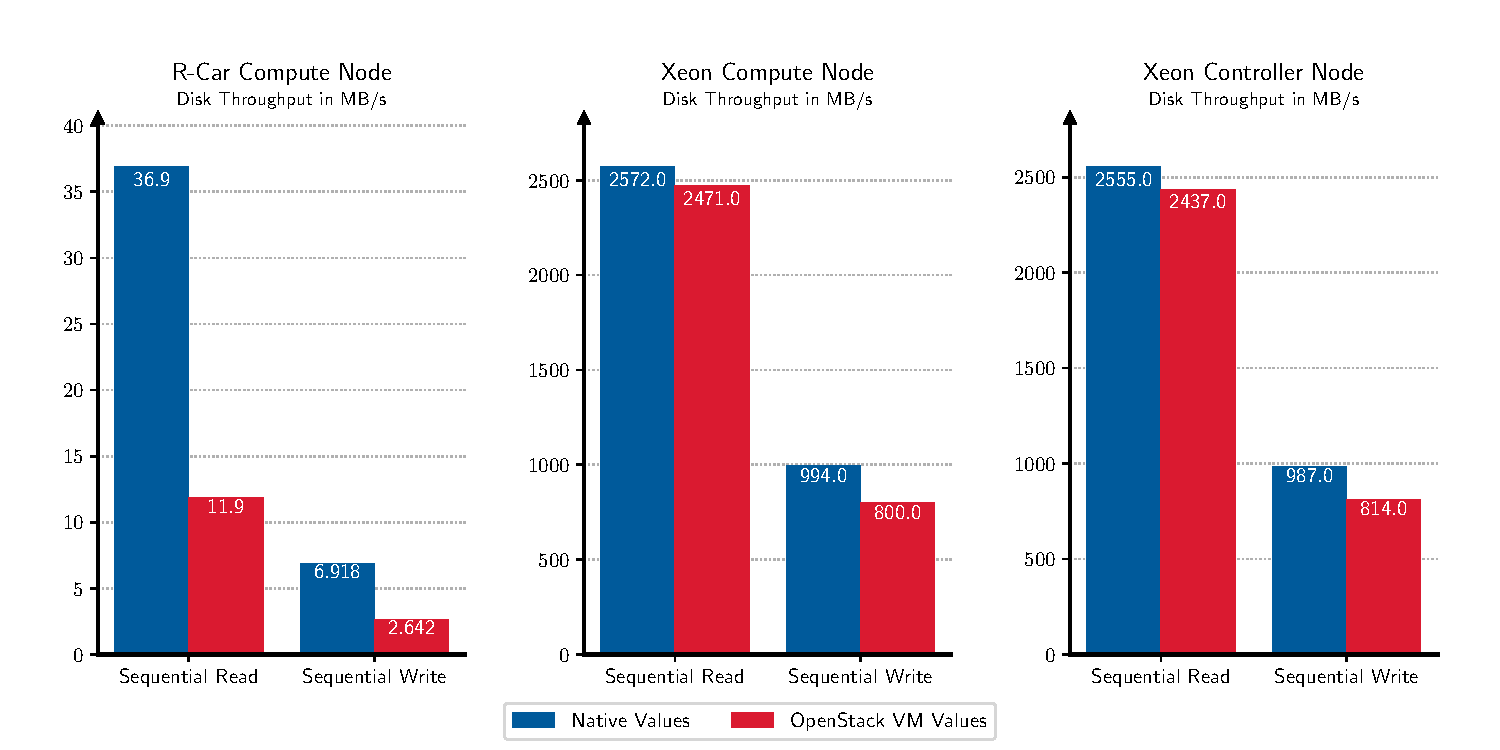
\includegraphics[width=\linewidth]{05_all-disk.pdf}
              \captionof{figure}{Storage performance on all tested platforms}
              \label{fig:all_disk}
            \end{figure} 

            \noindent As described in Section \ref{subsection:methodology_storage}, the platform's secondary storage's sequential read and write speeds were measured.
            Figure \ref{fig:all_disk} shows the native and \ac{VM} storage performance on all evaluated systems.
            Clearly visible, the R-Car has the worst performance in general and suffers the greatest performance impact.
            During testing, the SD-Card was found to achieve ambiguous results using different block sizes for testing. 
            Despite the SD-Card's general low performance, a block size of 128kb was found to deliver stable and consistent results.
            Inside the \ac{VM}, the storage suffers a 25 MB/s or 68\% performance impact regarding sequential read speeds.
            Also, sequential write speeds are impacted by 4 MB/s or 62\%.
            However, the measured values are not representative for two reasons.
            First, an SD-Card would not be used in a real-world scenario due to its low performance.
            Instead of SD-Cards, on-board storage like flash-storage or embedded multimedia cards would be used.
            The SD-Card was nevertheless chosen due to the easier handling regarding reflashing and reconfiguration of the host software.
            Second, because of the SD-Card's low performance, even little variation in performance yields a high percentage overhead.
            An impact of 25 MB/s on the Xeon platform would seem negligible, however, it makes a significant difference on the R-Car platform.
            Further tests using more suitable storage would very likely provide better and more accurate results.
            Especially the usage of the R-Cars' on-board flash storage would yield real-world values.
            However, this was not considered in this thesis due to the limited storage capacity of the on-board flash, the installation complexity using two partitions, and to preserve the \ac{SoC}'s flash of numerous reflashes.
            
            \noindent In contrast, the Xeon nodes feature an NVMe drive, enabling better insides on this platform.
            As the plots in Figure \ref{fig:all_disk} show, the performance is significantly better on native and virtual hardware.
            Both Xeon nodes show similar performance impacts.
            Regarding sequential read speeds, the \acp{VM} suffer a 100-128 MB/s or 4-5\% impact, while at sequential write speeds, the \acp{VM} suffer a 173-194 MB/s or 18-20\% impact.
            Commonly, write speeds are lower than reading speeds due to the actual process of changing and physically writing data to the storage device.  
            The low performance degradation regarding sequential read speed presents an acceptable overhead.
            However, the impact regarding the sequential write speeds is significant and not neglectable.
            
            \noindent Despite the bad results on the ARM platform and the high overhead for sequential writes on the x86 platform, the results have to be relativized.
            In an automotive embedded environment, apart from research with many measurements creating lots of data points, the data to be stored and read is relatively small.
            This makes full utilization of the available bandwidth unlikely.
            Further, the read speeds are more relevant and ensure a fast execution of applications, which is desirable and achieved by the x86 platforms.
            The x86 platform also depicts that OpenStack is capable of utilizing high-speed storage.
            The performance could be further increased utilizing OpenStack's object storage service \textsl{Swift} or enhancing the configuration towards storage performance.
            Also, a real-word test scenario would provide better reliability regarding the results.

           
        \subsection{Effects on the Memory}
        \label{subsection:memory_impact}
            
            \begin{figure}[ht]
              \centering
              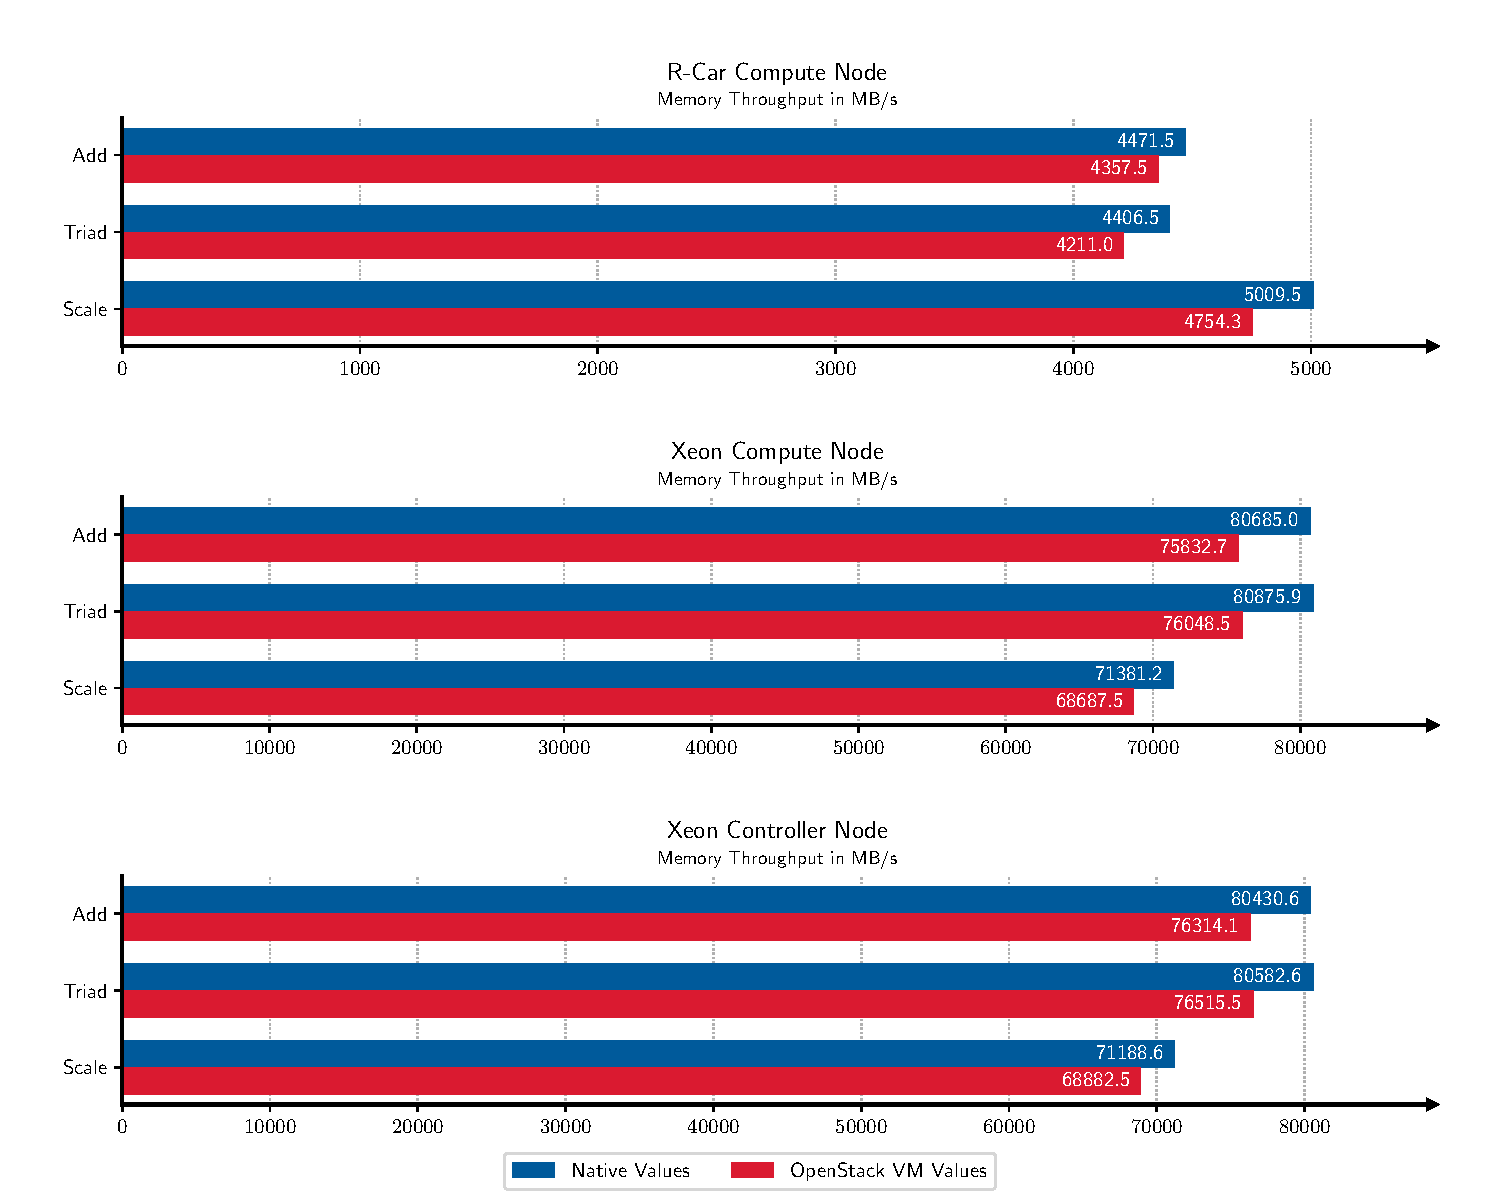
\includegraphics[width=\linewidth]{05_all-mem.pdf}
              \captionof{figure}{Memory throughput on all tested platforms}
              \label{fig:all_mem}
            \end{figure}
            
            \noindent Having measured the memory performance through mathematical operations according to Chapter \ref{subsection:methodology_storage}, Figure \ref{fig:all_mem} depicts the results.
            All \ac{VM} measurements are lower than the native ones.
            Due to being processed by more software layers compared to a native operation, \ac{VM} operations must be lower than native operations.
            The significantly higher throughputs on the Xeon systems reflect the higher thread count used on the Xeon nodes.
            However, dividing the values by the thread number yields values in pretty similar dimensions.
            
            \noindent On the R-Car node, OpenStack introduces an overhead of 3\% (add), 4\% (triad) and 5\% (scale).
            On the Xeon nodes, the introduced overhead lies in the same area at 3-6\%.
            Contrary to the R-Car node, the Xeon nodes' scale operation introduces a lower overhead of 3\% compared to the R-Car, where an overhead of 5\% is introduced.
            However, the native performance of the Xeon nodes' scale operation is in general lower compared to the two other operations, while on the R-Car, it is higher.
            This suggests that the ARM platform natively better supports such operations compared to the x86 platform.
            
            \noindent Overall, an overhead of 3-6\% on both platforms is plausible and acceptable. 
            This indicates excellent computational performance with little performance degradation. 
            Also, despite the R-Car's small memory, the performance is not impacted, further indicating good performance on systems with lower memory. 


        \subsection{Effects on the Network}
        \label{subsection:network_impact}
            
            \begin{figure}[ht]
              \centering
              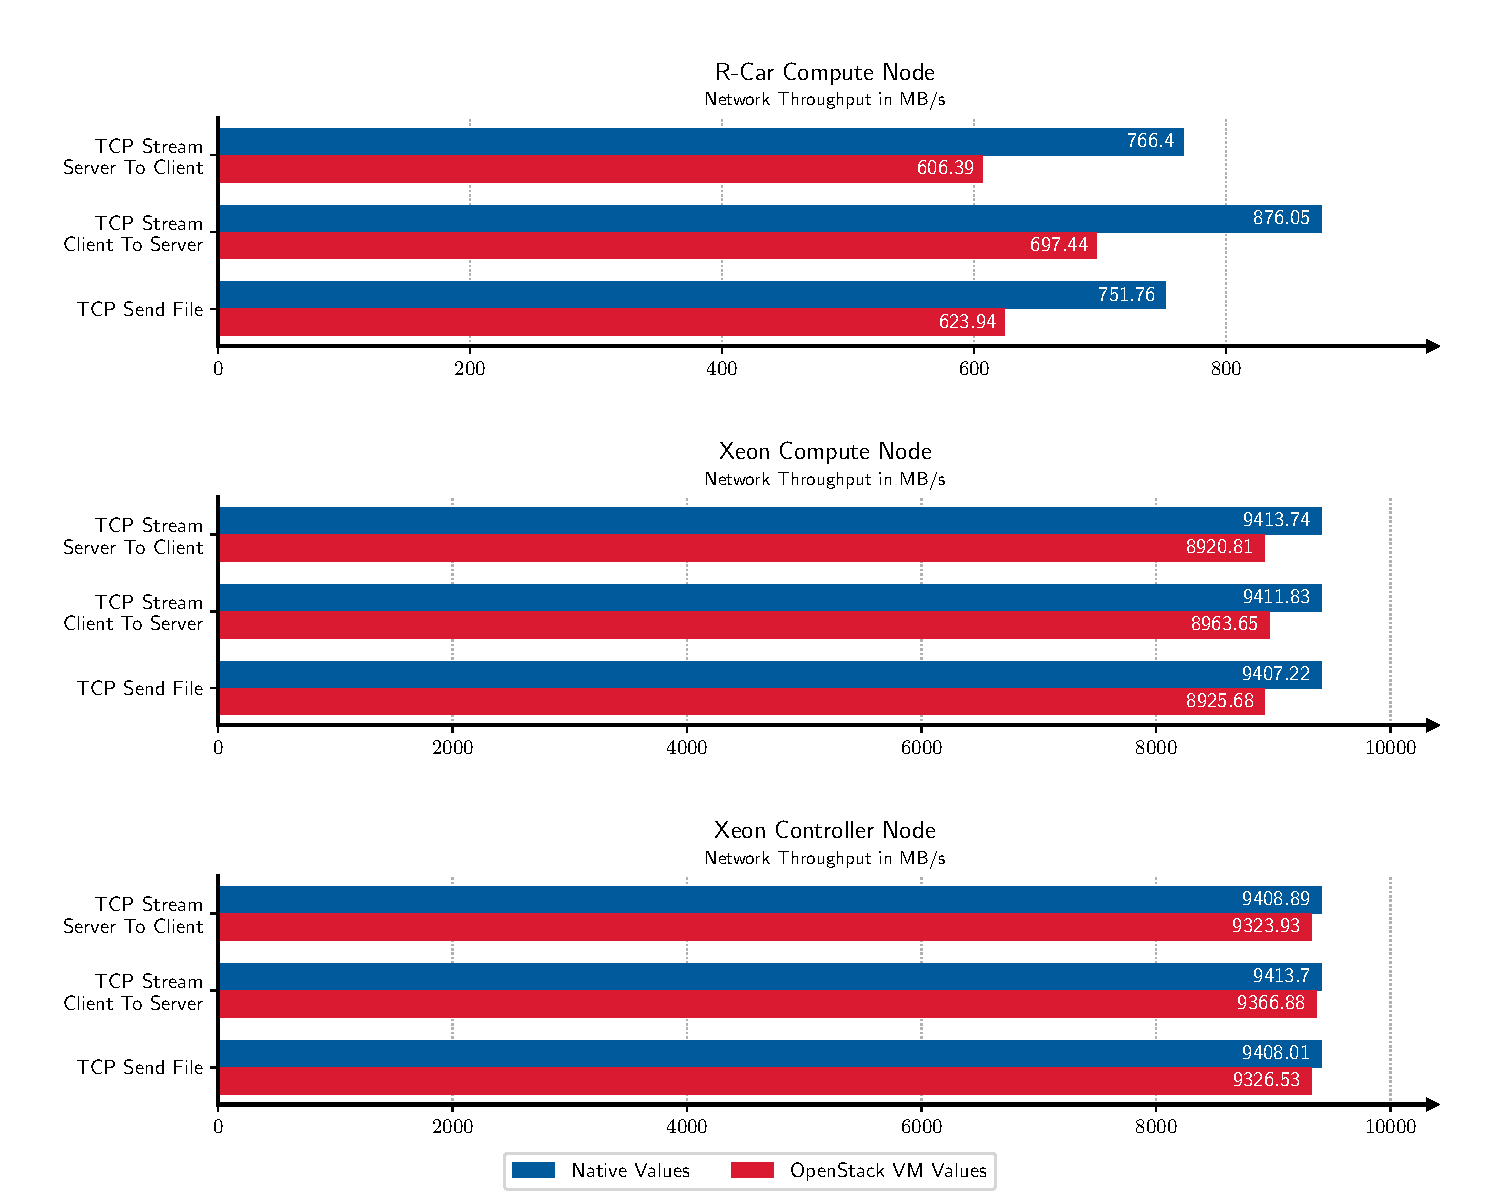
\includegraphics[width=\linewidth]{05_all-net.pdf}
              \captionof{figure}{Network throughput on all tested platforms}
              \label{fig:all_net}
            \end{figure}
            
            \noindent Studying the network throughput results in Figure \ref{fig:all_net}, all three tested platforms yield different results.
            First, the Xeon nodes yield much higher general performance due to their 10 Gbit connection.
            This already is a relevant finding as modern vehicles make more and more use of 1 Gbit and, in the future, probably 10 Gbit connections.
            The performed measurements show that OpenStack can handle these connections.
            On the other hand, the R-Car node is only equipped with a 1 Gbit network interface, yielding significantly lower results.
            
            \noindent The overhead lies at 20\% for the stream tests on the R-Car node and at 17\% for the file send test. 
            In all tests, the VM suffers a similar impact, which could be related to the R-Car's overall lower computing capabilities during the simultaneous usage of the high-performance cores by the host and guest.
            As described in \ref{subsection:cpu_impact}, the simultaneous resource usage by host and guest requires additional computational resources, as well as time, which reduces the throughput.
            In the context of network performance, additional services process data-packets before actually releasing them onto the network and vice versa.
            
            \noindent Examining the Xeon compute node, results with much lower overhead are found.
            For all tested connections, the overhead stays at about 5\%.
            This strengthens the indication that the host system's computational capabilities can influence network performance and lead to better results.
            Also, the results show that the VM utilizes the hardware and the 10 Gbit connection used. 
            
            \noindent Closing, the controller node delivers additional insides on the performance overhead.
            Regarding the test configuration, the environment differs in two points from the ones of the R-Car and the Xeon compute node.
            First, the compute services are now located on the same host as the OpenStack network service Neutron.
            This means that all requests can be directly processed by the same host and send out to the real world network without being first processed by a different node.
            Second, the Netperf-Server is now not being run on the controller node but on the Xeon compute node, making the controller node less utilized.
            This leads to an even lower overhead of only 1\% for all TCP connections.
            
            \noindent Considering the low and very low overheads of 5\% and 1\% on the Xeon nodes, the performance is again satisfactory.
            The Xeon controller node's performance raises the possibility of always executing the Neutron service and the Nova services along with each other.
            At the expense of other resources, this could provide nearly native performance if necessary.
            The significant overhead of 20\% on the R-Car, on the other hand, is not acceptable.
            However, in an automotive environment, the transferred data is relatively small, containing small pieces of information like signals.
            Therefore, high throughput rates might not always be the primary concern, but rather the latency.
            However, as with storage, OpenStack enables various network configurations and enhancements, which would improve network performance.
            In addition, the usage of an ARM platform with 10 Gbit Ethernet and higher computational power would most likely increase the comparability and reliability of the results.
            
            \begin{figure}[ht]
              \centering
              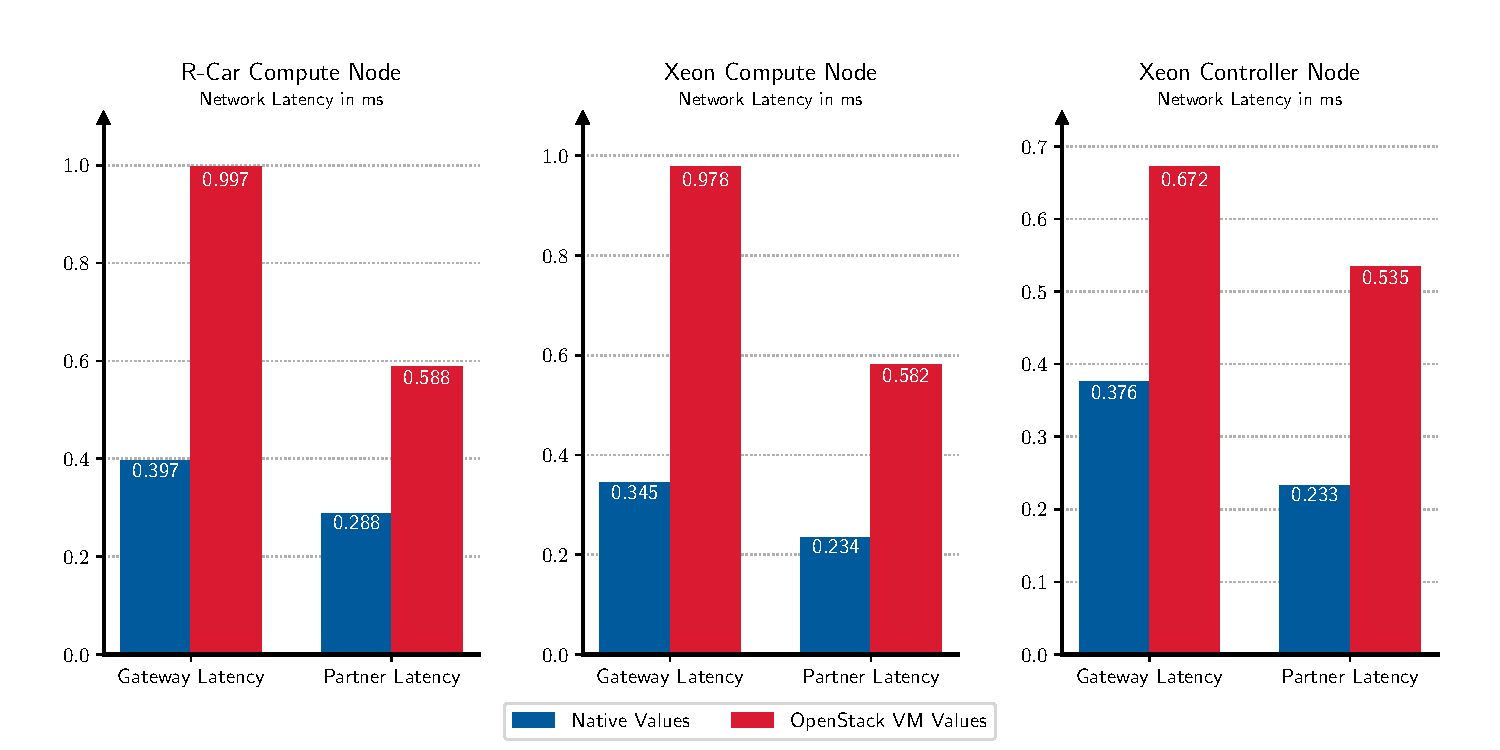
\includegraphics[width=\linewidth]{05_all-net-ping.pdf}
              \captionof{figure}{Network latency on all tested platforms}
              \label{fig:all_net_ping}
            \end{figure}
            
            \noindent Despite the different hardware and platforms, all performed latency tests yield very similar results in Figure \ref{fig:all_net_ping}.
            Pinging the gateway, a host not part of the OpenStack cluster, results in a latency measurement between 0.35 and 0.4 milliseconds.
            Pinging the Xeon controller and the Xeon compute node, hosts part of the OpenStack cluster, yields times about one millisecond shorter.
            This is accountable to the higher performance of the nodes versus the lower performance of the gateway.
            
            \noindent Regarding the measurements from inside the \ac{VM}, a clear overhead can be identified.
            Pinging the gateway, the R-Car, and the Xeon compute node yield a latency of about three times as high as natively.
            The Xeon controller node yields a latency of two times as high as natively.
            This overhead of about 200\% and 100\% can be attributed to the way OpenStack routes packets, in this case, ICMP packets, to their destination.
            Until the packets are released onto the real-world network, they are routed on an internal OpenStack network to the Neutron service host, in this case, the Xeon controller node.
            Arrived at the network node, the packets are processed by Neutron and only then released onto the real-wold network.
            The same situation applies to the replies in the backward direction.
            
            \noindent Executing the ping from the Xeon controller node VM gives the possibility to identify OpenStack's actual overhead.
            Because the controller VM packets are already on the controller hardware, only an one-time processing of them is necessary to place the packets on the real-world network.
            Taking 0.3 milliseconds more on the controller node for both pings, this 0.3 milliseconds are the actual overhead introduced by OpenStack.
            This also matches the fact that the overhead is twice as high with 0.6 milliseconds on the two compute nodes, as on those nodes, the packets have to be processed twice, on the compute host itself and on the network node.
            Considering further that the ping utility measures the round trip time, meaning from source to destination and back, the actual overhead is even smaller.
            OpenStack introduces an overhead of about 0.15 milliseconds from the Neutron service host and 0.3 milliseconds from other compute hosts for packets to reach their destination. 
            
            \noindent Considering the native values, 100\% and 200\% longer latency values are not negligible.
            Nevertheless, the measurements were performed on a local network and within a close range. 
            Real-world networks could introduce much longer latencies, making the native values much bigger.
            For example, a ping to the Google DNS server takes about 15 milliseconds.
            Considering an overhead of 0.3 or 0.6 milliseconds from an OpenStack \ac{VM}, the percentage overhead is only 2\% or 4\%, being well reasonable and acceptable.
            Being an extreme example as the packets have to travel a long distance shows that the actual overhead compared to the native hardware can vary on a different network.
            To gather real-world values, the test should be performed on an actual automotive network with a real-word load.

    \section{Summary}
    \label{section:summary}
        
        Concluding from the performed results, OpenStack clearly introduces an overhead in all considered domains.
        However, on both evaluated platforms, the VMs function consistently and reliably. 
        
        \noindent The Xeon systems represent a significantly more powerful embedded platform which delivers very high performance.
        OpenStack's impact on this platform is relatively small, and little performance degradation is measured. 
        This suggests an actual in-vehicle use.
        The R-Car results, in contrast, do not show such good performance.
        Considering the high performance degradation of the CPU and secondary storage, an in-vehicle use seems not promising.
        However, the network and memory performance measurements show that good performance is achievable on the R-Car and the degradation does not apply generally.
        This promises better and improved performance on different hardware with better components like faster secondary storage and more CPU cores.
        
        \noindent Despite the overhead, all functionality is continuously available, enabling the consideration of OpenStack's advantages in the following chapter.
        This chapter identified and evaluated the major negative impacts and disadvantages of OpenStack: the overhead and performance degradation.
        However, neither the better nor the worse performance of the platforms used do entirely prevent further tests or the in-vehicle usage in general. 

\chapter{Use Cases}
\label{chapter:usecases}
    
    Apart from a small impact and overhead on resources, OpenStack should also function reliably and as anticipated.
    Therefore, also advantages and new features have to be measured and evaluated.
    Considering the typical environment of OpenStack being, for example, a data center with usual hardware, embedded systems like automotive \acp{ECU} do not belong in this category.
    Nevertheless, OpenStack must perform reliable and consistent to benefit from its features and possibilities of Cloud Computing.
    As exemplary advantages of OpenStack in the context of automotive embedded systems, two scenarios are examined and measured.
    The following sections describe which value OpenStack can introduce through \ac{VM} distribution and migration.
    The measurements are performed using Python scripts to interact with the OpenStack cluster using the OpenStack Python SDK.
    All scripts used can be found at \cite{Malinowski2021}.
    
    
    \section{VM Distribution}
    \label{section:distribution}
        
        OpenStack enables the automatic distribution of \acp{VM} according to defined rules.
        While currently applications are bound to \acp{ECU}, they cannot be executed elsewhere.
        However, this would come in handy if, for example, an individual \ac{ECU} is highly loaded while another does not have much to process.
        By pooling the available resources and distributing them, \acp{VM} can be executed independently on the most suitable hardware.
        The functionality should work as intended, otherwise, unforeseeable complications could occur, leading to, for example, overloaded \acp{ECU}.
        
        \noindent The distribution on those platforms is evaluated separately because of specific instruction sets and, therefore, specific images for the ARM and x86 nodes.
        The Nova-Scheduler being responsible, among other things, for the assignment of \acp{VM} to hosts, can be configured by various parameters.
        For the evaluation of \ac{VM} distribution, the following parameters are modified.
        
        \newpage
        \begin{itemize}
            
            \item \textsl{scheduler\_driver\_task\_period} \hfill \\ 
            This parameter sets the interval of how often the scheduler updates its resource information.
            A smaller interval means better and more accurate values but also an increased overhead as the information must be polled more often from the compute nodes.
            
            \item \textsl{cpu\_weight\_multiplier} \hfill \\ 
            This parameter sets the importance of used \ac{CPU} cores.
            A positive multiplier will try to achieve even distribution with an even number of cores used on every host.
            A negative multiplier will first use all available cores on one compute node before utilizing the next one.
            
            \item \textsl{ram\_weight\_multiplier} \hfill \\ 
            This parameter sets the importance of used memory.
            A positive number will try to achieve even memory utilization on all hosts. In contrast, a negative number will try to first utilize all available memory on one host before moving on to the next one.
            
            \item \textsl{disk\_weight\_multiplier} \hfill \\ 
            Similar to the cpu\_weight\_multiplier and ram\_weight\_multiplier, this parameter sets the importance of disk utilization.
            A positive number will again try to distribute VMs evenly based on the hosts' disk usage, while a negative number will first stack the VMs on one host. 
            
            \item \textsl{build\_failure\_weight\_multiplier} \hfill \\ 
            This parameter describes how much build failures of \acp{VM} on hosts influence the \ac{VM} assignment.
            The higher the value specified, the more build failures weigh, resulting in hosts with recent build failures not being chosen for a new \ac{VM} in the first place.
            
            \item \textsl{io\_ops\_weight\_multiplier} \hfill \\ 
            Like the previous weight\_multipliers, this parameter considers the \ac{CPU} usage on the compute nodes.
            If a positive value is defined, compute nodes with high \ac{CPU} utilization will be chosen over ones with low utilization.
            On the other hand, a negative value configures the scheduler to chose low-utilized nodes over high-utilized ones.
            
        \end{itemize}
        
        
        \subsection{Distribution Scenarios}
        
            On both platforms, two different and contrary distribution strategies are tested.
            First, an equal distribution regarding the \ac{CPU} cores is tried to be achieved.
            As the CPU cores are one source of computational performance, equal distribution among all compute nodes would decrease each compute node's CPU load.
            This would prevent the \ac{VM} performance from being degraded due to the host being too highly loaded.
            Second, a stacked distribution regarding the \ac{CPU} cores is tried to be achieved.
            Configuring the scheduler to first use all available \ac{CPU} cores on one compute node until utilizing a second node would enable to set these nodes into a standby or low power mode.
            Due to this, energy could be saved as not all nodes would be necessarily utilized all the time.
            Table \ref{table:distribution_parameters} shows the parameter configurations for both distribution strategies.
            
            \begin{table}[ht]
                \begin{center}
                    \begin{tabular}{l|c|c}
                        \textbf{\makecell[c]{Parameter}} & \textbf{Stacked Distribution} & \textbf{Equal Distribution} \\
                        \noalign{\hrule height 1.5pt}
                        scheduler\_driver\_task\_period 		&	5		&	5 \\
                        cpu\_weight\_multiplier			&	5.0		&	-5.0 \\
                        ram\_weight\_multiplier 			&	5.0		&	-5.0 \\
                        disk\_weight\_multiplier			&	5.0		&	-5.0 \\
                        build\_failure\_weight\_multiplier		&	5.0		&	0.0 \\
                        io\_ops\_weight\_multiplier 		&	-1.0		&	5.0
                    \end{tabular}
                \caption{Nova-Scheduler parameters for VM distribution}
                \label{table:distribution_parameters}
                \end{center}
            \end{table}
            
            \noindent The \ac{VM} flavors used are the smallest defined, being the \textsl{rcar-01-128-06} and the \textsl{xeon-06-21504-106} flavor.
            In order to best evaluate the distribution, as many \acp{VM} as possible should be spawned and distributed.
            With the ARM cluster having only 16 cores in total, this was the highest number of machines possible.
            To keep the Xeon cluster comparable and the testing time reasonable, it was also decided to spawn 16 machines.
            Therefore the flavors representing one-eighth of the total resources were chosen.
            
            \noindent The scenario measurements are performed in the following way:
            On each cluster, 16 \acp{VM} are created and started sequentially.
            For every \ac{VM}, during its creation, the \ac{VM}'s compute host is checked.
            This way, the initially scheduled host by the Nova-Scheduler is captured, as well as any host changes due to build failures.
            The scenario is performed one time with each scheduler configuration.
        
        
        \subsection{Scenario Evaluation}
            \begin{figure}[ht]
              \centering
              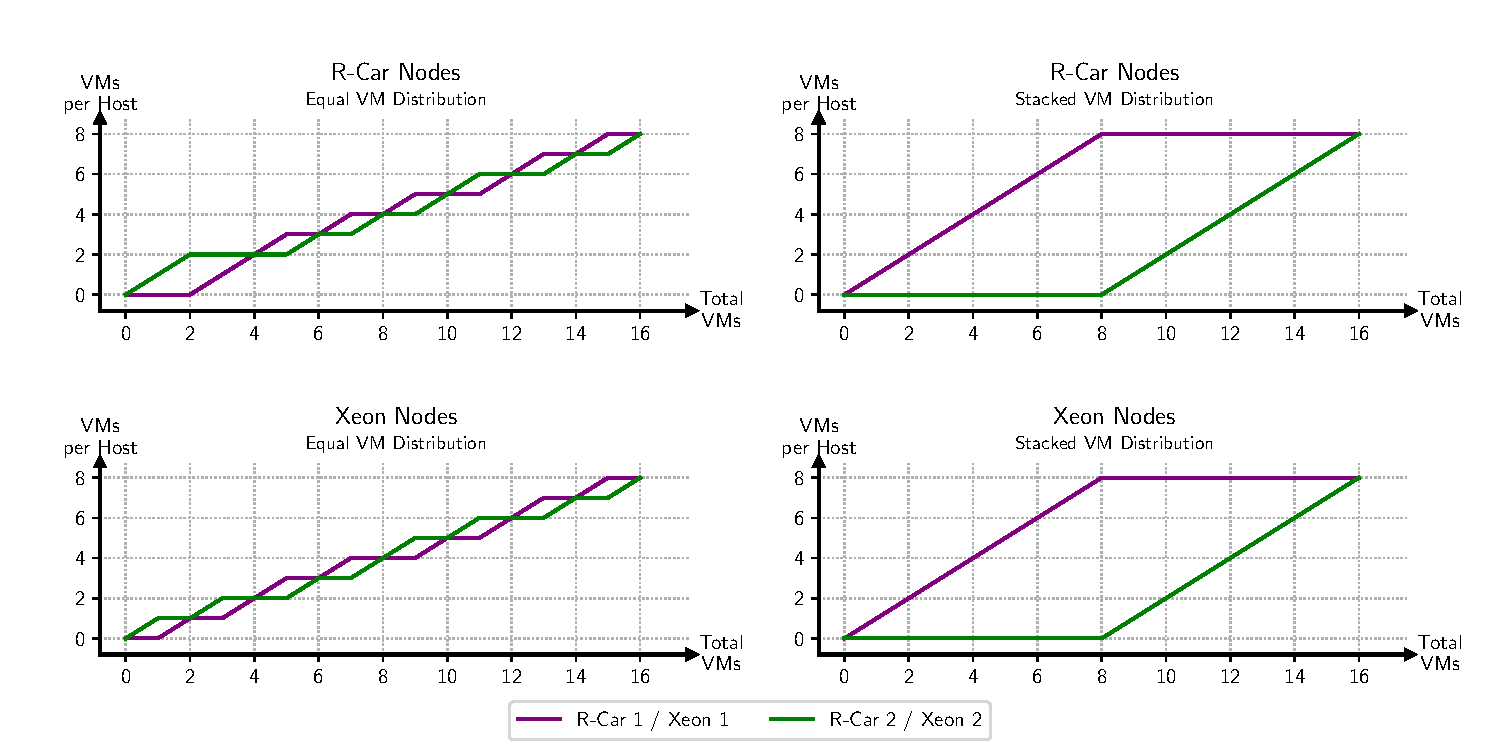
\includegraphics[width=\linewidth]{06_all-distribution.pdf}
              \captionof{figure}{VM distribution across compute nodes}
              \label{fig:vm_distribution}
            \end{figure}
            
            \noindent Figure \ref{fig:vm_distribution} shows the \ac{VM} distribution across the R-Car cluster (top row) and the Xeon cluster (bottom row).
            First and foremost, no errors or host reschedules are visualized in the plots as no errors or reschedules occurred.
            For all distributions and hosts, the spawning was always successful.
            Further, it is clearly visible in the figure that the different distribution scenarios worked and were realized as expected by the Nova-Scheduler.
            
            \noindent The right column of Figure \ref{fig:vm_distribution} shows the stacked distribution.
            The first eight VMs are clearly assigned to the R-Car 1 / Xeon 1 compute node, while the last eight VMs are assigned to the other compute node.
            The left column shows the equal \ac{VM} distribution. 
            Obviously, over time the \acp{VM} are distributed equally across the two nodes.
            On the R-Car cluster as well as on the Xeon cluster, the distribution is not strictly alternating during the equal distribution, depicted by the first two \ac{VM} assignations to the R-Car 1 node.
            Also, the 10th and 12th \ac{VM} are assigned to R-Car 1 in a row.
            Similar behavior can be seen on the Xeon cluster: \acp{VM} 4 and 5, 8 and 9 and 12 and 13 are assigned to the same compute node in a row.
            However, as the number of running \acp{VM} per host is the same, a selection of the same hosts twice in a row is not false, as both hosts are equally utilized.
            
            \noindent The correct functionality of the \textsl{io\_ops\_weight\_multiplier} is captured in the first \ac{VM} assignment on the Xeon cluster to the Xeon 2 node.
            Xeon 1, being the controller, is more utilized, and therefore Xeon 2 is chosen over Xeon 1.
            However, striking are the first two \ac{VM} assignments to the R-Car 2 node using an equal distribution (Figure \ref{fig:vm_distribution}, top-left plot). 
            Assigning the second \ac{VM} also to the R-Car 2 node indicates that the \ac{CPU} of R-Cars 1 is higher utilized at that time, as it has to outweigh the \ac{CPU}, memory, and disk multiplier.
            However, the third and fourth \ac{VM} are assigned to the R-Car 1 again, balancing the distribution again.
            
            \noindent Concluding, both scenarios show that a distribution strategy on embedded hardware for \acp{VM} is possible.
            Also, the absence of reschedules and build errors demonstrates the reliable operation of OpenStack.

        
    \section{VM Migration}
    \label{section:migration}
  
        \noindent A large number of \acp{ECU} in today's vehicles brings two essential advantages.
        The presence of multiple \acp{ECU} brings redundancy and enables to group functionality on particular \acp{ECU}.
        In case of an \ac{ECU} failure, another \ac{ECU} can continue its work to avoid security and safety implications.
        Similarly, real-time software can be separated from less time-critical software to avoid interference or performance degradation.
        While the separation or grouping can be achieved easily and with various OpenStack methods, the aspect of redundancy can also be satisfied by OpenStack.
        Similarly, multiple \acp{VM} could calculate the same task on different hosts in parallel, realizing today's approach.\\
        Yet, OpenStack further enables a different approach to deal with, for example, instance failures.
        By executing all functionality inside \acp{VM}, these \acp{VM} are decoupled from the hardware and can be migrated to other hosts.
        This can happen by transferring a switched-off instance but also a live, currently active instance.
        Therefore, if an \ac{ECU} being a compute host fails or a problem is detected, its \acp{VM} can be migrated to other running hosts. 
        As valuable as live-migration might sound, the performance during it must not be impacted too much to provide value, and the duration must be reasonable.
        While \acp{VM} are shifted to another compute host, the resources are in a state without one single defined host.
        As the resources are either partly on two hosts or for a short time on neither host, the performance could suffer drastically.
        Also, depending on the resources used by the \acp{VM}, the duration could take an unacceptable amount of time.
   
   
    \subsection{Time}
    \label{subsection:usecases_time}

        \noindent To evaluate the live-migration duration of \acp{VM}, a Python script is executed.
        The script boots a \ac{VM} on one host and flowingly migrates it to another host.
        Same as the \ac{VM} distribution, the migration time is evaluated separately for the R-Car and the Xeon cluster. 
        Using the OpenStack Python SDK, the VM's status is periodically polled, and the interval between entering and leaving the \textsl{migrating}-status is used for evaluation.
        To ensure the instances are migrated between the right hosts, only the compute services on the relevant hosts are active during the migration.
        The migrations are performed with all configured flavors in order to discover potential impacts of resources on time.
        
        \subsubsection*{Time - Evaluation}
        
            \begin{figure}[H]
              \centering
              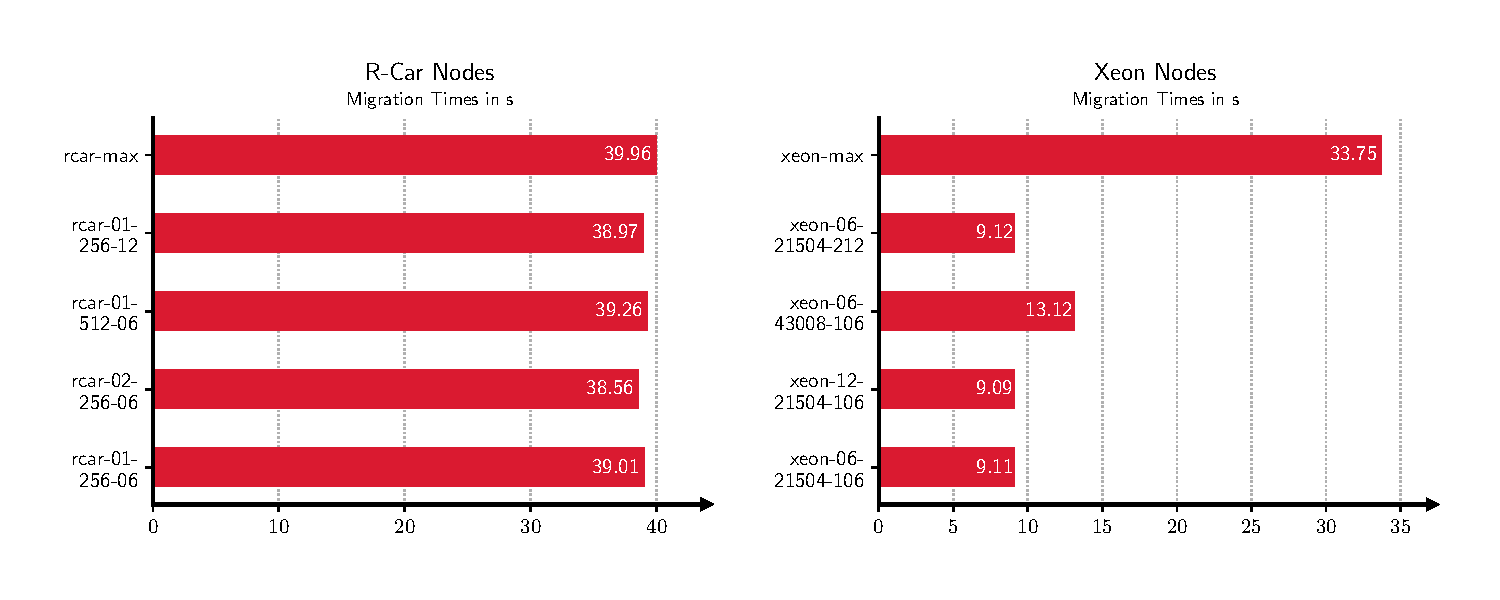
\includegraphics[width=\linewidth]{06_all-migration.pdf}
              \captionof{figure}{VM migration times}
              \label{fig:vm_migration_time}
            \end{figure}
            
            \noindent Figure \ref{fig:vm_migration_time} shows the migration times for the R-Car and Xeon cluster.
            While on the R-Car nodes, all flavors take about 40 seconds to migrate, on the Xeon nodes, the flavors need about 10 seconds, except the \textsl{max}-flavor taking about 34 seconds.\\
            Considering the Xeon migration times, one resource can be identified as exceptionally time-consuming.
            All flavors except the \textsl{max}-flavor represent a twofold increase of one resource compared to the smallest flavor \textsl{xeon-06-21504-106}.
            Neither double the CPU cores nor double the disk size seems to affect the migration time significantly.
            Double the memory, however, extends the migration time by three seconds.
            Considering now the \textsl{max}-flavor needing 34 seconds together with the fact that a memory increase of 21504 MB increases the duration by three seconds, memory seems to have the most significant impact.
            Therefore, for the total migration time of the \textsl{max}-flavor, 24 seconds (8*3 seconds) are necessary only to migrate the memory, while the remaining resources need ten seconds in total.\\
            Due to the \acp{VM} being in an idle state, neither the \ac{CPU} nor the memory or the disk is utilized.
            This explains why neither resource increase is directly reflected in an increased migration time.
            As the actual amount of resources to migrate stays the same, no actual increase in resource usage is present, and therefore no change is introduced.
            However, while the memory utilization is also not differing from flavor to flavor, it nevertheless has an impact, leading to the conclusion that the memory has to be freed on the old host and allocated in some way on the new host.
            
            \noindent Using these conclusions, the overall low performance and the little to no variation in migration time on the R-Car cluster can be explained.
            Striking, no substantial difference in migration time between the smallest, the biggest, or any other flavor can be identified.
            Also, a substantial influence of the memory size is absent.
            This suggests that the migration time is mainly influenced by something else.
            Considering the fact that all \acp{VM}, on the Xeon and on the R-Car nodes, where started using local storage, everything is existing and stored locally on the current host.
            Flowingly, everything has to be transferred to the destination host accordingly during the migration. 
            On the one hand, this explains the not changing migration times on the Xeon Cluster with increased storage because the actual data size stays the same.
            On the other hand, the Xeon nodes are connected via a 10 Gbit Ethernet connection, while the R-Car nodes have only a 1 Gbit connection.
            This leads to the fact that no variation in migration on the R-Car cluster can be identified because the storage migration always influences the migration time the most.
            Having a ten-times slower connection and less powerful hardware, the storage migration takes more time than anything else.
            
            \noindent In current vehicles, 1 Gbit Ethernet connections are already present, and using 10 Gbit capable hardware will be the next step to follow.
            Together with powerful hardware, reasonable migration times can be achieved.
            Taking into account that memory requirements, as well as storage requirements, are kept as low as possible in embedded software, the performance would further increase.
            However, a utilized CPU and memory might additionally impact the migration time, as examined in the next section. 
        
        
    \subsection{Performance}
    \label{subsection:usecases_performance}
    
            \noindent Considering live-migration in a redundancy use case, besides the reliability and the migration time, the performance during it is critical.
            Depending on the use case and its requirements, either continuation or performance or both may be favored.
            For example, in a time-critical real-time software, the performance must not be impacted, as this would make the application indeterministic and could lead to catastrophic events.
            In the case of an application with less strict timing requirements like an infotainment application, however, the functionality's continuation is more important, even if the performance is slightly reduced for a short amount of time.
            
            \noindent The \ac{CPU} being the primary computational resource, it was decided to gather values about the \ac{CPU} performance.
            In order to achieve this, the \textsl{Sysbench} benchmark\footnote{Sysbench Benchmark: https://github.com/akopytov/sysbench} is used.
            The benchmark uses prime number factorization to determine \ac{EPS} and latency values of the \ac{CPU}.
            Considering these values over time during a live-migration, a statement about the performance is possible.\\
            The values are collected as follows:
            First, a \ac{VM} is created, and all software updates inside it are performed.
            Next, the Sysbench benchmark is installed using aptitude.
            The Sysbench benchmark is configured to factorize as many prime numbers as possible for one second, every two seconds.
            The flavor with the doubled \ac{CPU} core number is used on both clusters, and the number of threads used by Sysbench is specified to be half the number of available cores.
            This provides \ac{EPS} and latency values every two seconds so that a complete visualization of the migration performance can be established without losing any significant values.
            The \ac{VM} is run for 2 minutes on one compute host and flowingly migrated to the other host in its cluster.
            This is performed four times so that four migrations are captured.
        
        
        \subsubsection*{Performance - Evaluation}

            \noindent Figure \ref{figure:vm_migration_performance} shows the collected values.
            Visible in both clusters are the \ac{EPS} drop and the latency spike during the migrations.
            However, the absence of a definite plateau in the \ac{EPS} and latency plot indicates no measurement values were lost, and the impact only lasts a short amount of time.
            Further, both clusters' migration durations increase compared to the results in Figure \ref{fig:vm_migration_time}.
            On the R-Car cluster, using the \ac{VM} flavor \textsl{rcar-02-128-06}, the migration time increases from 40 seconds to 100 seconds (best case) or 150 seconds (worst case).
            Similarly, on the Xeon cluster, using the \ac{VM} flavor \textsl{xeon-06-21504-106}, the migration time increases from 10 seconds to 17 seconds (best case) or 30 seconds (worst case).
            This clearly shows that a non-idle \ac{VM}, having a utilized \ac{CPU} takes longer to migrate than an idle \ac{VM}.
            Additionally, Figure \ref{figure:vm_migration_performance} shows that Xeon 1, in general, achieves lower EPS and higher latency values running the core services.
            
            \begin{figure}[H]
                \centering
                \begin{subfigure}[b]{\textwidth}
                    \centering
                    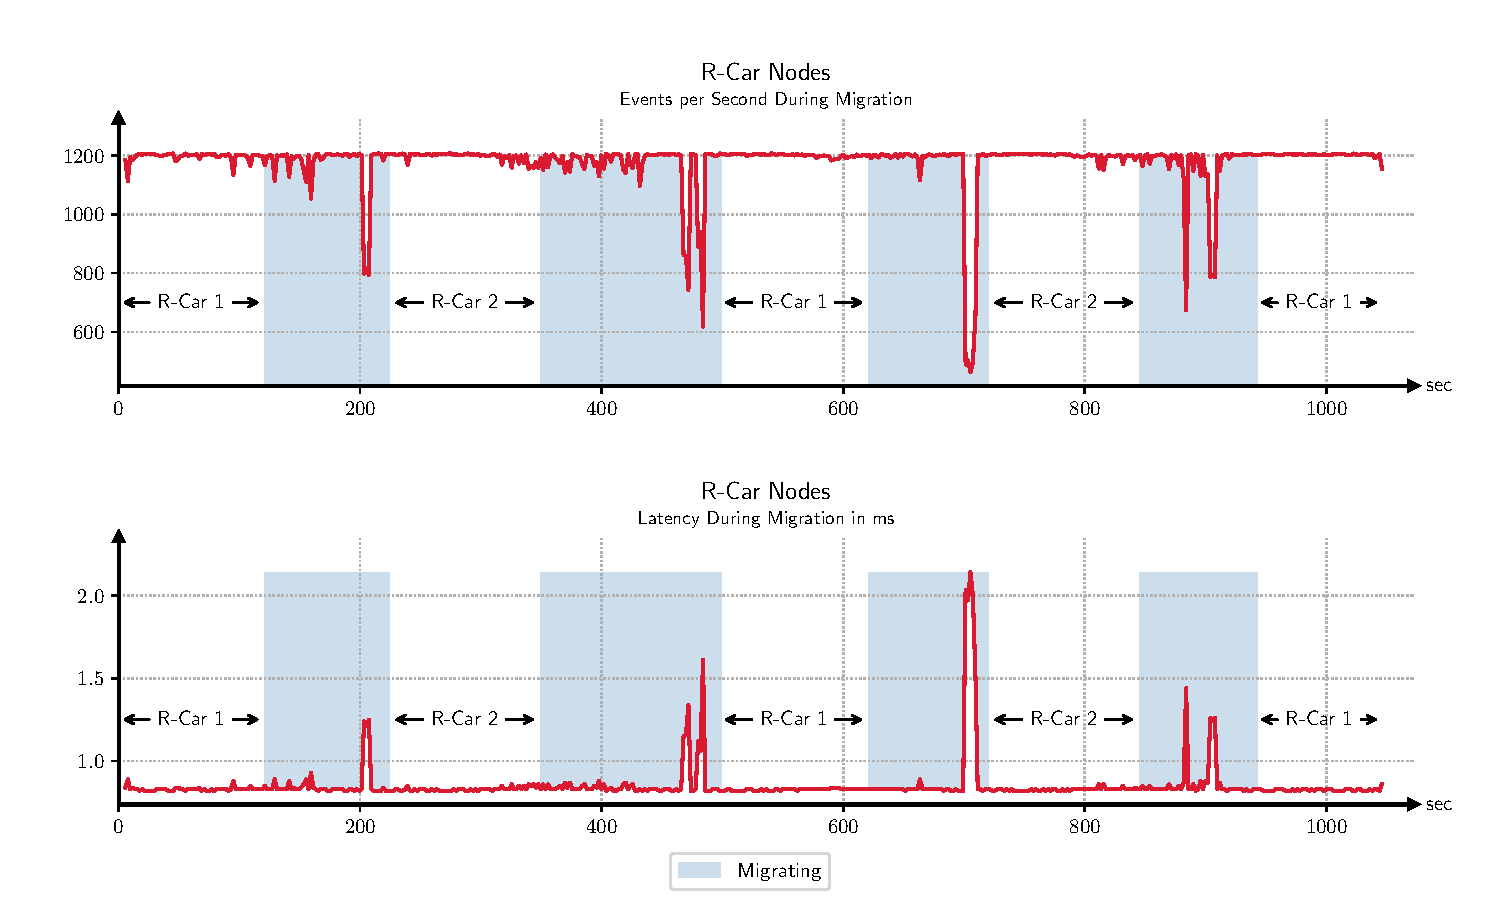
\includegraphics[width=\textwidth]{06_rcar_cluster_migration_performance.pdf}
               \end{subfigure}
               \caption[]{VM migration performance on the R-Car and Xeon cluster}
            \end{figure}%
            \begin{figure}[ht]\ContinuedFloat
                \centering
                \begin{subfigure}[b]{\textwidth}
                    \centering
                    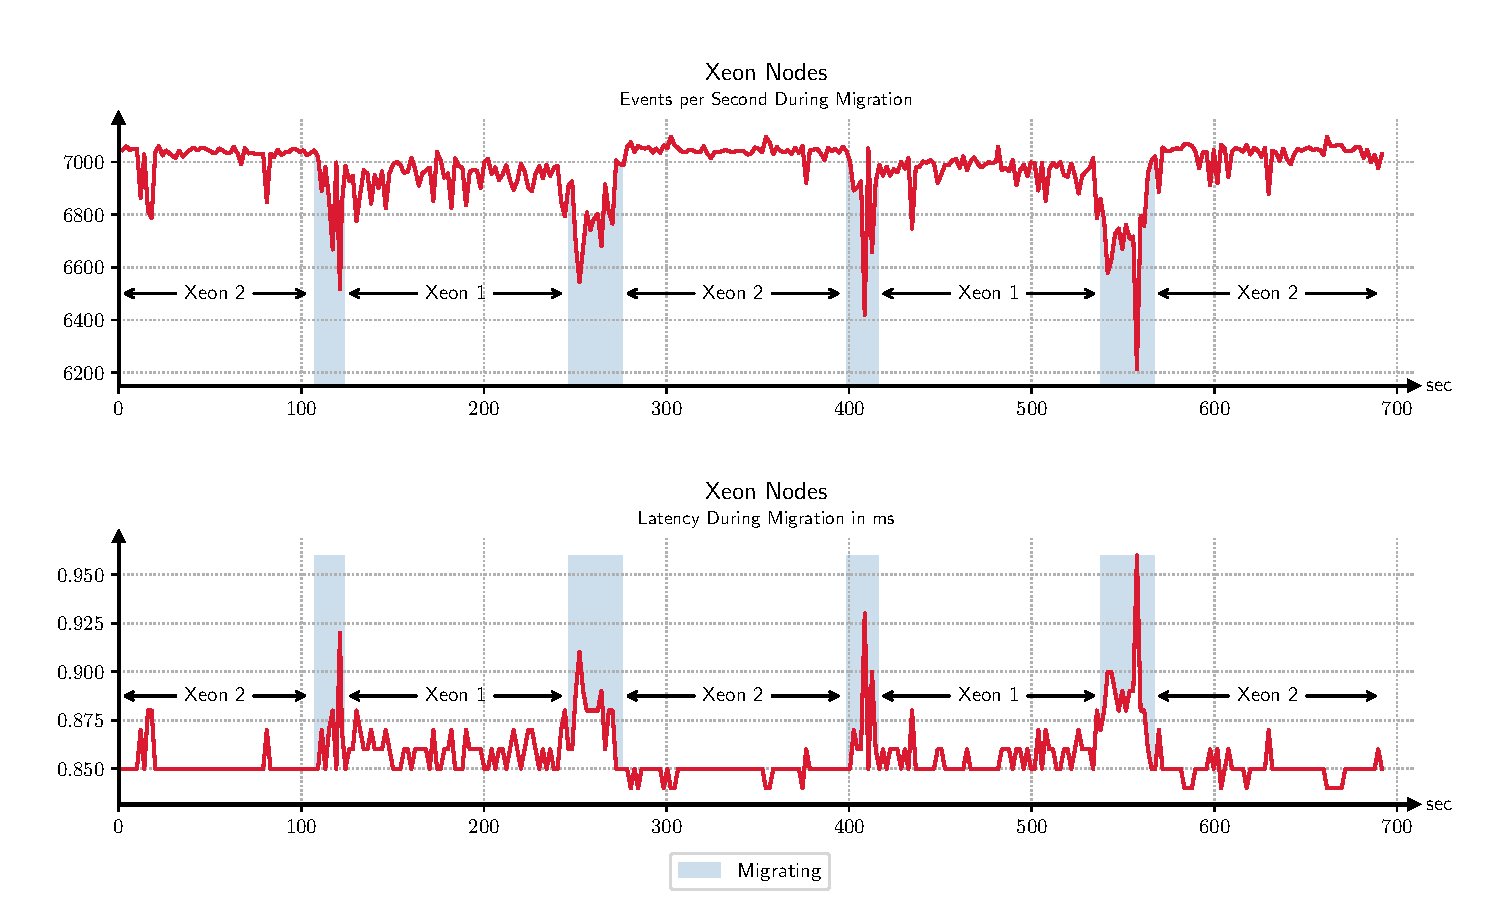
\includegraphics[width=\textwidth]{06_xeon_cluster_migration_performance.pdf}
                \end{subfigure}
                \caption[VM migration performance on the R-Car and Xeon cluster]{VM migration performance on the R-Car and Xeon cluster (cont.)}
                \label{figure:vm_migration_performance}
            \end{figure}

            \noindent Examining the plot in detail, it can be seen that the performance degradation, in general, is only given for a concise amount of time, even when the migration itself takes much longer.
            The peak EPS drops only last for a couple of seconds on the R-Car and the Xeon nodes.
            This is very noticeable on the R-Car nodes.
            Due to only executing one thread on the R-Car nodes, only when this specific thread or rather \ac{CPU} core is migrated, the \ac{EPS} number drops.
            Nevertheless, the drop from 1200 \ac{EPS} to 800-520 \ac{EPS} corresponds to a performance degradation of 33-52\%, being non-negligible even in short time frames if performance is critical.\\
            On the Xeon nodes, the degradation is not as significant as on the R-Car.
            Due to executing three threads, the peak performance drops during the migration are less significant.
            On the Xeon nodes, the performance drops by 400-800 \ac{EPS}, corresponding to a 5-10\% performance impact.
            This leads to the finding that multi-threaded processes and parallelized applications suffer lower performance degradation during a live-migration compared to single-threaded processes.
            As threads seam to be migrated one after another, improved fundamental performance through more threads or higher single-core performance lowers the percentage degradation.
            
            \noindent Considering the latency, the spikes correspond precisely to the \ac{EPS} drops.
            Reasonably, the EPS number drops if the CPU has a higher latency, meaning that fewer requests can be carried out per time frame if the CPU takes longer to react to a request.
            However, the R-Car latency spikes are much higher (2 milliseconds) compared to the Xeon spikes (0.1 milliseconds).
            This can be attributed to the fact that first, the Xeon \ac{CPU} is more powerful, and second, executing three threads leads to a high probability of some thread always reacting quickly to a request.
            The influence of multiple threads can be seen in the fact that the time interval in which the \ac{EPS} number drops is much longer compared to the R-Car cluster.
            While on the Xeon cluster the performance degradation is present for a longer duration, the R-Car cluster suffers a higher but shorter degradation.
            Nevertheless, on both clusters the rise in \ac{CPU} latency inhibits a usage for real-time applications, as the CPUs' responsiveness becomes indeterministic. 
            
            \noindent Further, the graphical representation of the migration confirms the previous section's statement regarding the time share of different resources.
            The figure shows that the \ac{CPU} is migrated last as the spikes and drops appear at the end of the migration.
            Especially, the R-Car plot shows that the \ac{CPU} migration happens in a concise time frame compared to the total duration. 
            As the total duration increases in contrast to the previous section, the memory impact on the migration time is further hardened.
            The CPU and memory utilization being the only difference to the measurements in Section \ref{subsection:usecases_time}, their utilization can be made responsible for the longer migration time.
            
    
    \subsection{Application Migration}
    \label{section:usecases_application}
        
        Having examined the migration time and performance in the previous sections, an actual application shall be migrated.        
        Since real-time and hard-safety applications would require further and more complex tests, these are out of this thesis's scope.
        Nevertheless, the previous measurements and scenarios suggest that an OpenStack cluster on automotive hardware is realizable.
        To demonstrate this, it was decided to evaluate the migration of a Tetris application.
        Being a small game, this represents the use case of playing a game on a vehicle's infotainment system.
        Not having hard real-time requirements but mainly regarding the quality of service, this reflects the previously described choice of a continuous function over high performance.
        However, the performance should still be as good as possible.

        \noindent This use case is evaluated in a similar manner as the migration performance in the previous section.
        However, as the Tetris game requires a more sophisticated user interface, the VMs must be prepared accordingly.
        A desktop shall represent the user interface which would also be present in an actual infotainment system.
        As the Ubuntu Cloud Images do not initially include a desktop, it first has to be installed.
        Further, a \ac{VNC} server is installed inside the \ac{VM}.
        This enables the remote access of the machine's desktop and its interaction.
        As Tetris game, the game \textit{Quadrapassel}\footnote{Quadrapassel Game: https://wiki.gnome.org/Apps/Quadrapassel} from the Ubuntu repository was chosen due to its easy installation via aptitude and low hardware requirements.\\
        In order to evaluate this scenario, two different measurements are performed.
        First, using the resource usage measurements from Section \ref{section:methodology_idle}, the overhead and resource usage with an active application inside the \ac{VM} are examined.
        Second, the same measurements are performed during the live-migration.
        Only one migration is measured as multiple migrations do not provide more information but only extend the test time.
        
         \subsubsection*{Application Resource Usage - Evaluation}
        
            \noindent Before the migration, Figure \ref{figure:use_case_usage} shows the resource usage on the compute hosts R-Car 2 and Xeon 2.
            In addition to the tests from Section \ref{section:evaluation_consumption}, in this measurement, the \acp{VM} are not left idle after creation, but the \ac{VNC} server and the application are started.
            Figure \ref{figure:use_case_usage} enables a clear distinction between the different actions performed while preparing the system before migration. 
            In addition, to Figure \ref{fig:all_idle}, through measuring the \ac{CPU} and memory usage inside the \ac{VM} too, even better visualization of OpenStacks overhead is possible.
            Regarding the R-Car node, an overhead of 2\% in \ac{CPU} usage and an overhead of 100 MB in memory usage is found.
            For the Xeon node, the \ac{CPU} overhead also lies between 1-2\% during an active application, while the memory overhead lies at about 4 GB.
            Also visible, the \ac{CPU} and memory usage only rise significantly if the usage inside the \ac{VM} rises, apart from small periodic peaks due to periodic OpenStack processes.
            Further, the figure shows the difference between the \ac{VM} startup and the OS's actual boot inside the \ac{VM}.
            On the R-Car cluster, the duration between the \ac{VM} startup and the actual \ac{VM} boot is significantly longer than on the Xeon cluster.
            As explained in Section \ref{section:evaluation_consumption}, this originates from the higher computational power of the Xeon platforms.
            
          
        
       
        \subsubsection*{Application Migration - Evaluation}
            
            \noindent Figure \ref{figure:use_case_migration} shows the \ac{CPU} and memory usage on the R-Car and Xeon hosts during the live-migration.
            First and foremost, the live-migration succeeds.
            The player is able to continue to play the game throughout the whole migration without significant interruption.
            The game lags for a couple of seconds only towards the end of the migration, leading to inputs from the keyboard and outputs from the screen being slightly delayed.
            This fits together with the gained knowledge on the performance during a live-migration.
            As the performance drops towards the end, also the game performance drops.
            However, the game is not interrupted entirely and is available throughout the migration.
            
            \begin{figure}[H]
                \centering
                \begin{subfigure}[b]{\textwidth}
                    \centering
                    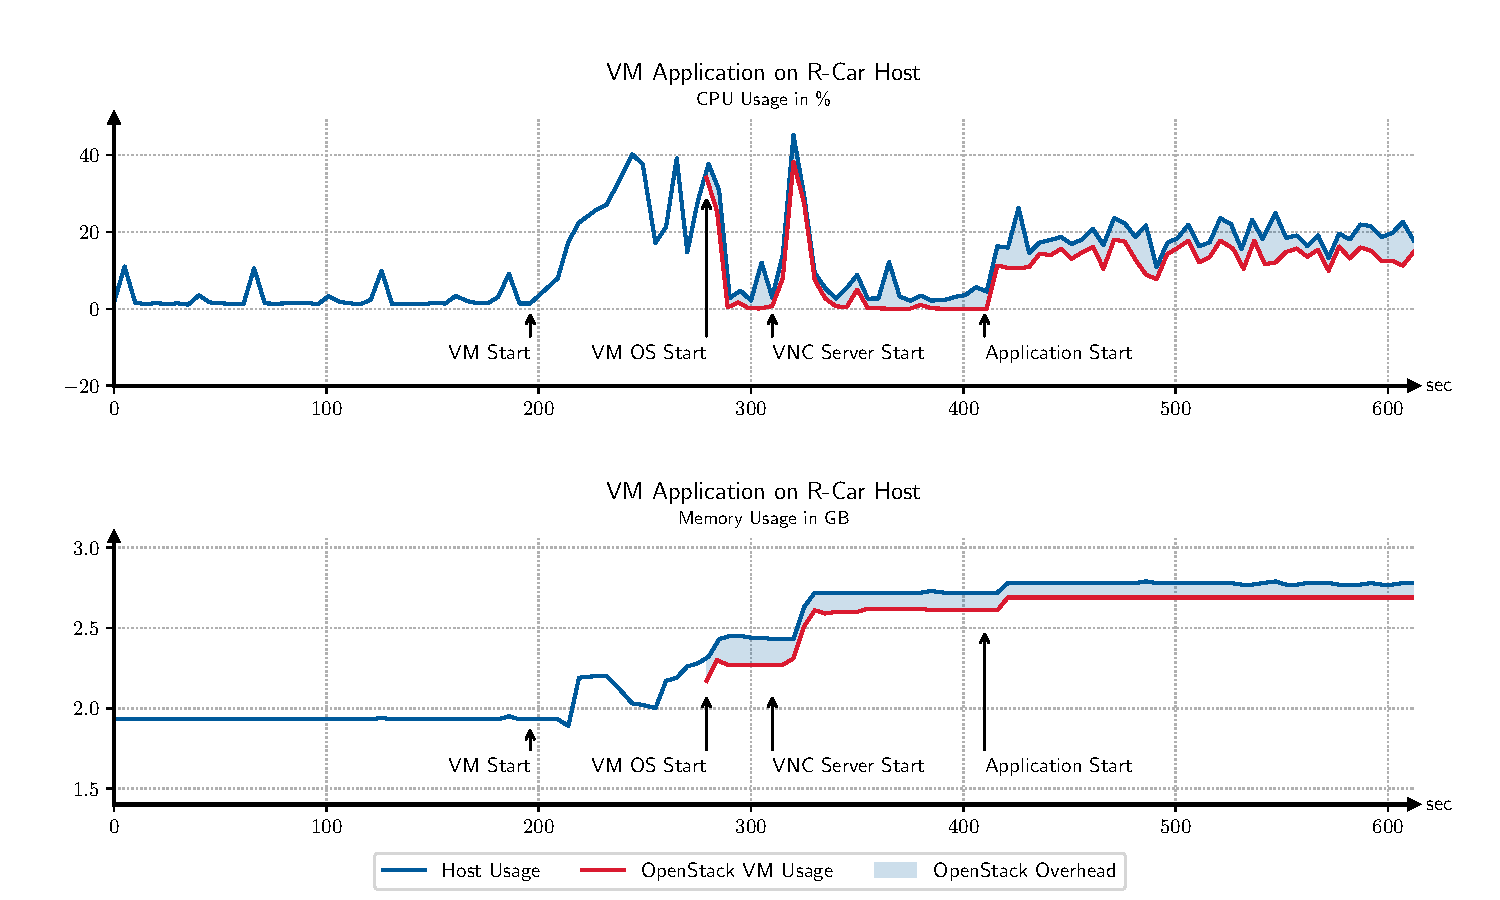
\includegraphics[width=\textwidth]{06_use-case-usage-rcar.pdf}
                \end{subfigure}
                \begin{subfigure}[b]{\textwidth}
                    \centering
                    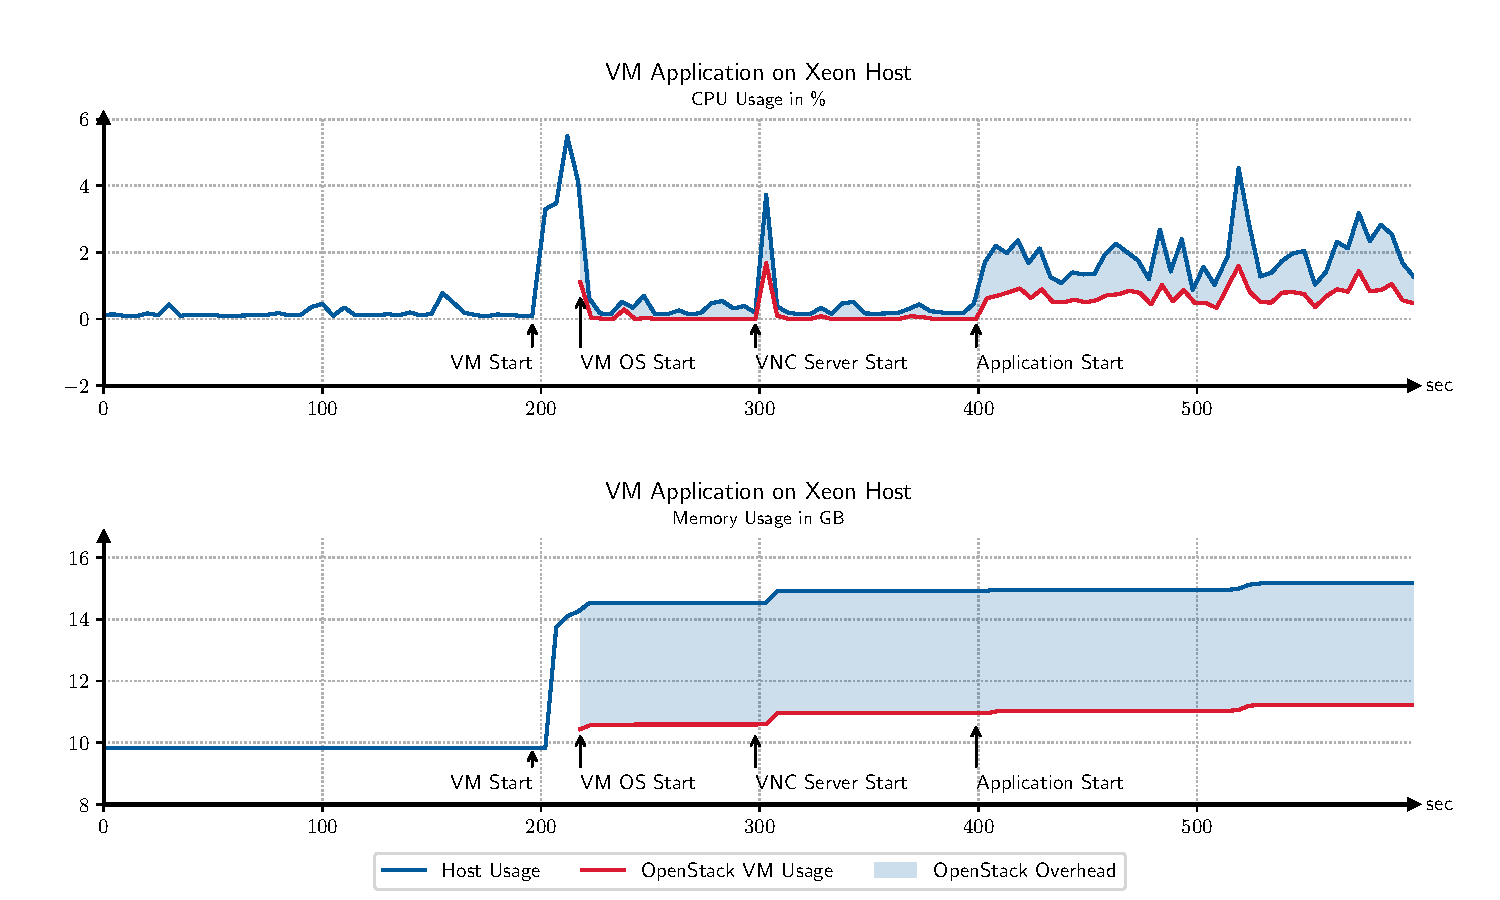
\includegraphics[width=\textwidth]{06_use-case-usage-xeon.pdf}
                \end{subfigure}
                \caption{R-Car and Xeon resource usage with VM application}
                \label{figure:use_case_usage}
            \end{figure}
            
            
            \noindent Examining the results in detail, the R-Car cluster duration shows as most striking.
            Taking about 1850 seconds or 31 minutes, it is significantly higher compared to the duration measured in Section \ref{subsection:usecases_time} and \ref{subsection:usecases_performance}.
            However, this is due to the limited resources on the R-Car.
            The measured memory values show that the use case requires 3.5-3.6 GB of memory, which corresponds to the R-Car's maximum available memory.
            As from this point on, the swap-memory is used, the operations are much slower, resulting in a significantly longer migration duration.
            As the disk data has to be migrated too, it first has to be read into memory before transferring it over the network.
            Using the much slower secondary storage as swap-memory results in a significant performance impact leading to the long migration time.
            Also, zooming into the memory usage reveals that the memory is transferred towards the end, depicted by the destination host's continuously growing memory usage.
            Further, the CPU usage illustrates that only the CPU usage on the destination host increases while the source’s CPU usage does not seem unusually affected by the migration.
            Clearly visible, the \ac{CPU} usage of the destination host is around 0\% in the beginning, while in the end, the source host shows a \ac{CPU} usage of about 0\%.
            The same behavior can be seen regarding memory usage.
            
            \begin{figure}[H]
                \centering
                \begin{subfigure}[b]{0.93\textwidth}
                    \centering
                    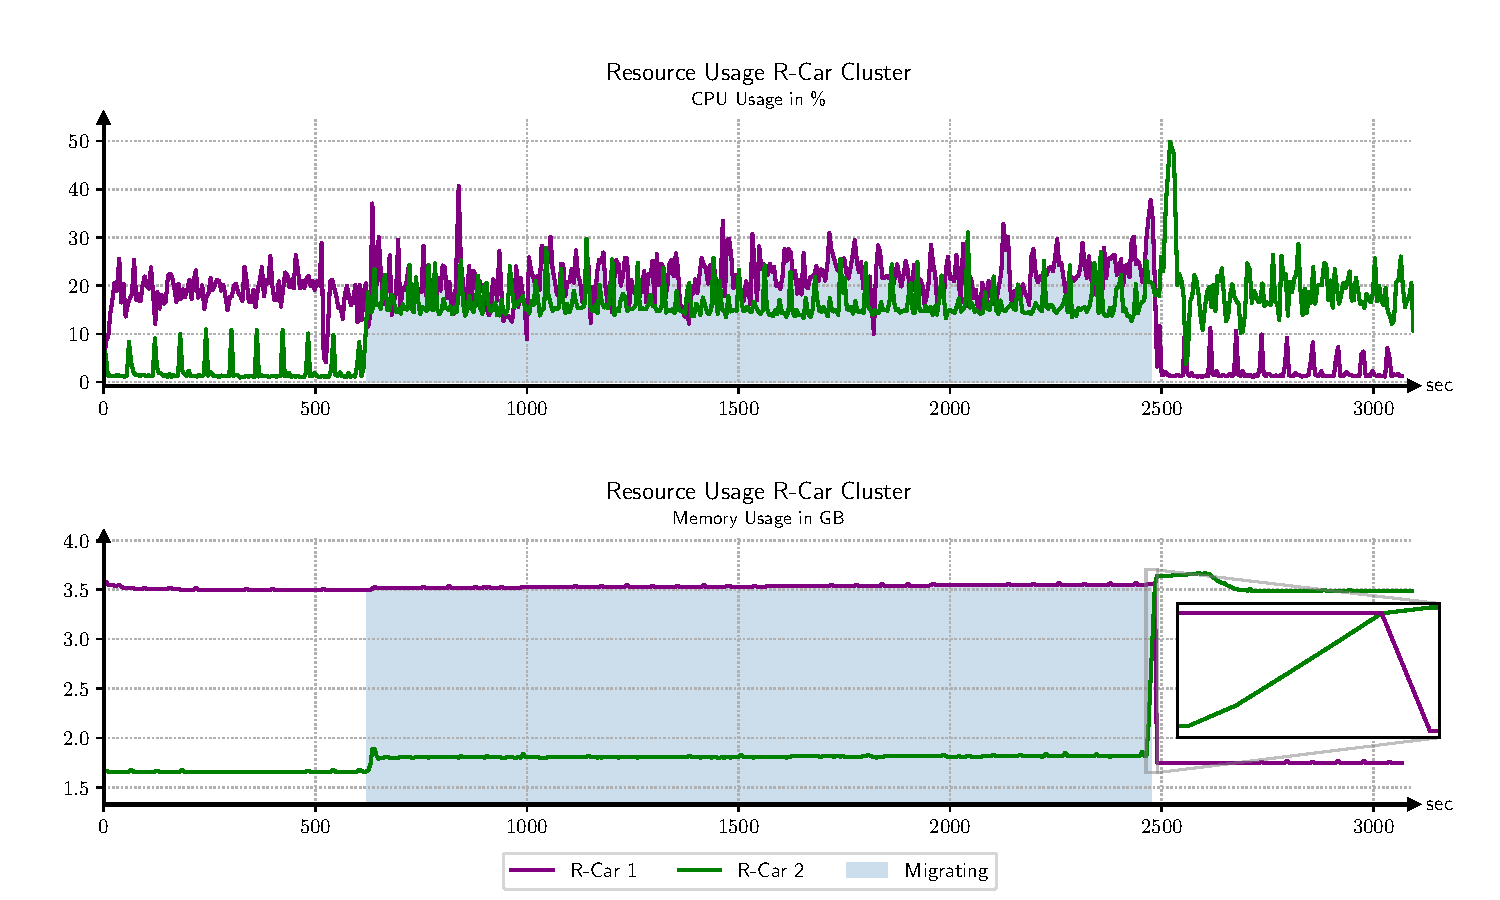
\includegraphics[width=\textwidth]{06_use-case-migration-rcar.pdf}
                \end{subfigure}
                \begin{subfigure}[b]{0.93\textwidth}
                    \centering
                    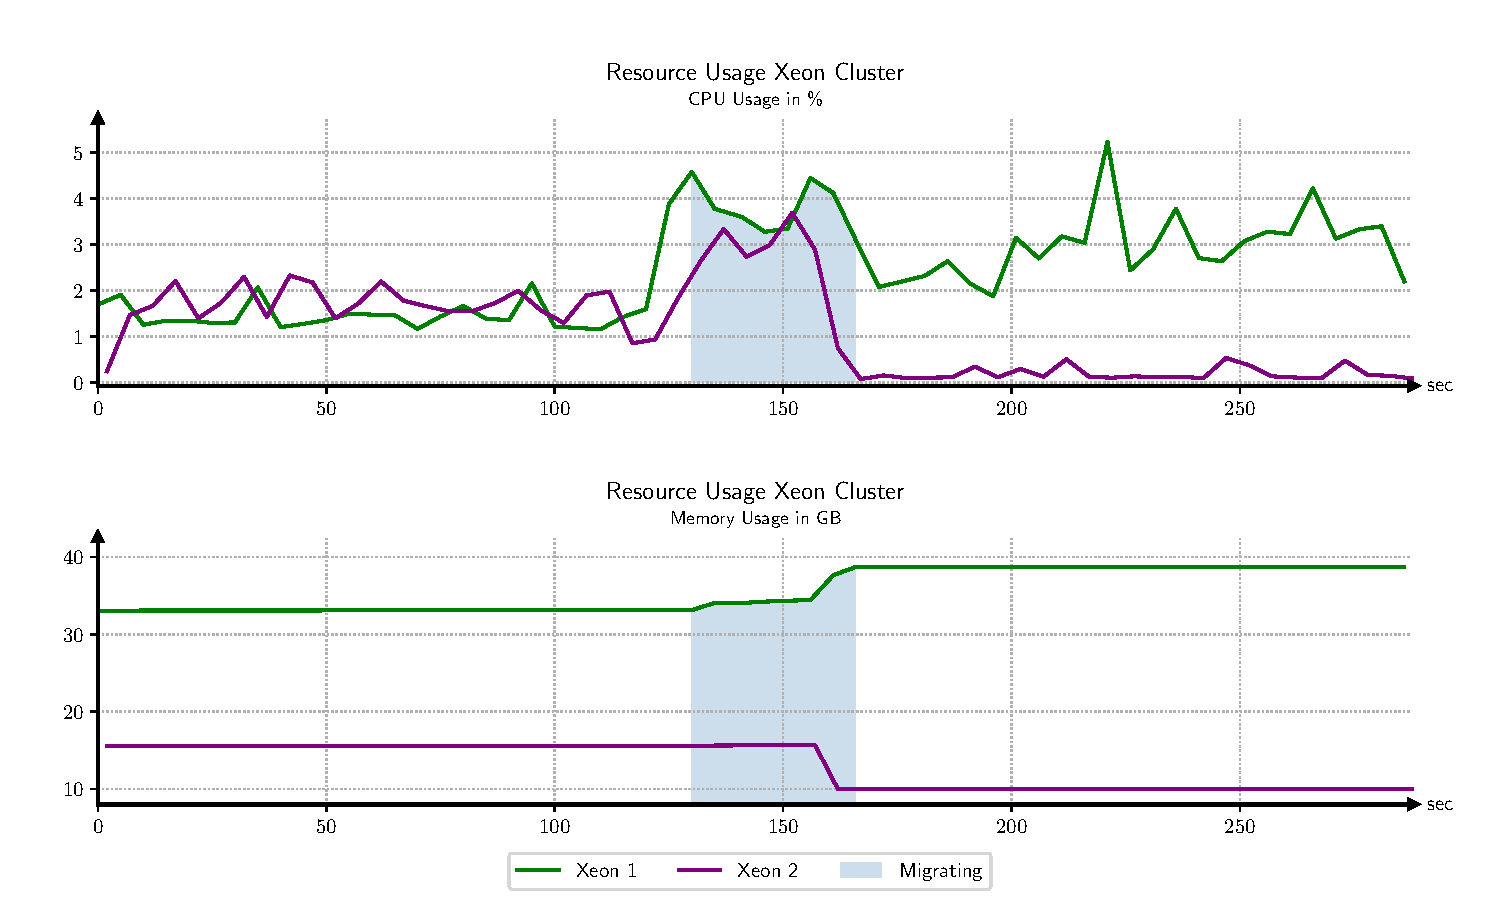
\includegraphics[width=\textwidth]{06_use-case-migration-xeon.pdf}
                \end{subfigure}
                \caption{R-Car and Xeon resource usage with VM application and migration}
                \label{figure:use_case_migration}
            \end{figure}
            
            \noindent The Xeon cluster, on the other hand, shows noticeable better and more confident results.
            Comparing the migration duration with results from Section \ref{subsection:usecases_time}, the times only differ slightly.
            While the idle \ac{VM} needs 34 seconds, the \ac{VM} with an active application takes only 3 seconds or 8\% longer.
            As on the R-Car cluster, Figure \ref{figure:use_case_migration} shows the host's additional \ac{CPU} and memory usage during the migration.
            However, contrary to the R-Car cluster, the live-migration affects the destination host and the source host on the Xeon cluster.
            As the migration happens significantly faster on the Xeon cluster, the \ac{CPU} has more load, which explains the not existing \ac{CPU} usage increase on the R-Car cluster.
            Due to the long duration, the R-Car \ac{CPU} can process all instructions over a longer period of time, leading to a lower overall load.
            Also, the increased fundamental \ac{CPU} and memory load through the control services is visible.
            
            \begin{figure}[H]
              \centering
              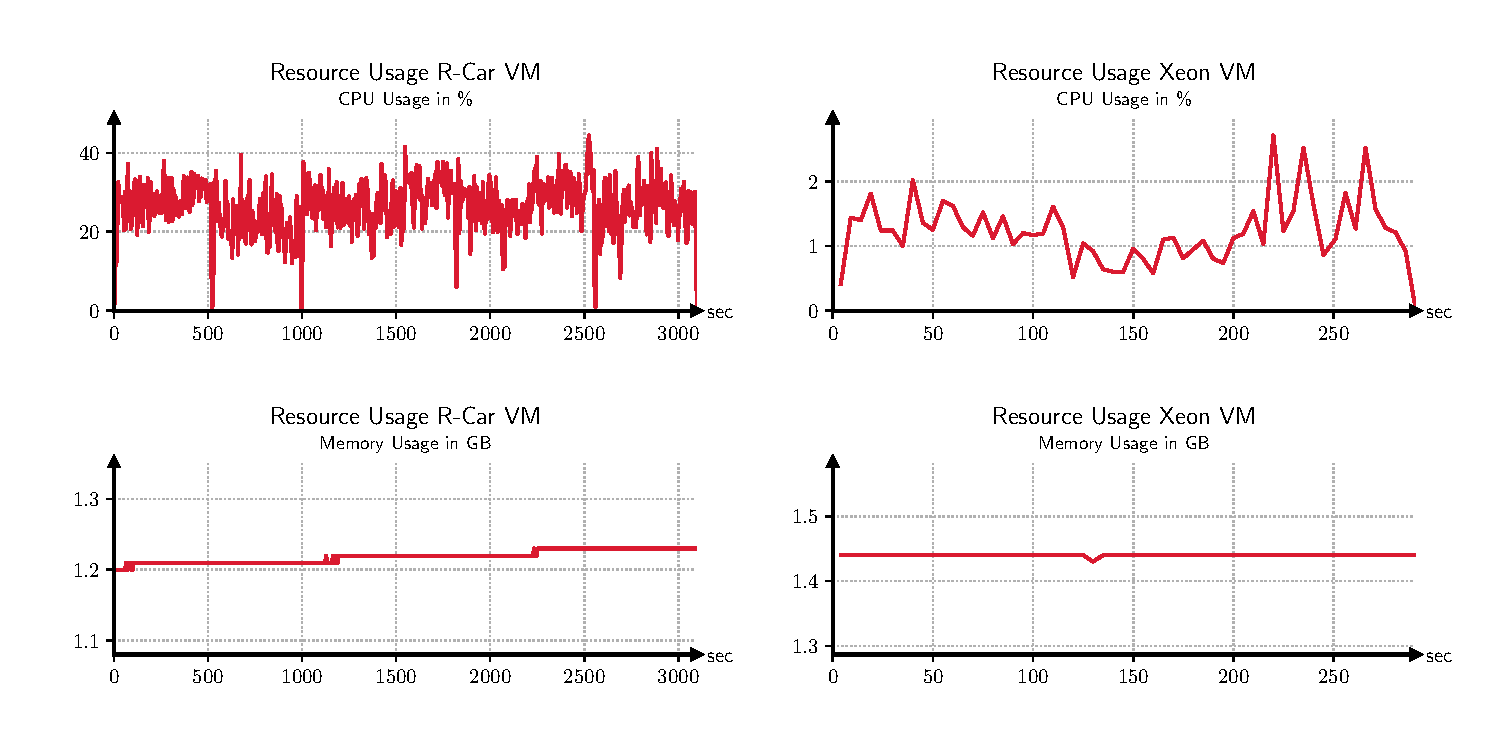
\includegraphics[width=\linewidth]{06_use-case-migration-vm.pdf}
              \captionof{figure}{VM resource usage with VM application and migration}
              \label{fig:use_case_migration_vm}
            \end{figure}
            
            \noindent Finally, Figure \ref{fig:use_case_migration_vm} additionally shows the \ac{CPU} and memory usage of the migrated \acp{VM}.
            The plots show no visible increase in \ac{CPU} or memory usage.
            This underlines that the live-migration does not affect the resource usage inside the \ac{VM}, but only on the host.
            
            \noindent In summary, the R-Car cluster results clearly show the unsuitability for a live- migration in a host failure case.
            Due to the very long duration, the host would have most probably already failed before the complete \ac{VM} would be fully migrated.
            On the Xeon cluster, on the other hand, the migration time is significantly lower.
            Also, the used \ac{VM} flavor represents an improbable \ac{VM} configuration, indicating even lower migration times using smaller \ac{VM} flavors.
            Therefore, the results suggest actual usability of the live-migration functionality if the hardware is powerful enough.
            
    \section{Summary}
        
        \noindent Concluding from the two examined use cases, OpenStack's advantages can be exploited.
        On both platforms evaluated, the tested functionality is reliably and continuously available.
        However, the smaller resources on the R-Car nodes along with the not advantageous big.LITTLE architecture and slow-performing SD-Card, counteract a performable operation of OpenStack.
        While the performance doesn't influence the VM distribution, VM migration is greatly influenced.
        As migration times with idle VMs seem to be just in an acceptable range, further measurements show the influence of active VMs on the migration time.
        With migration times spanning multiple minutes up to half an hour, this is not practicable in a real-world scenario and therefore doesn't introduce additional value.
        Powerful hardware, in contrast, is able to perform the migration in reasonable time frames, even with very large VMs.
        This allows the assumption that also the ARM platform would achieve better results with more resources available.
        Figure \ref{figure:use_case_migration} depicts that more memory, for example, 8 or 16 GB, could already suffice to achieve reasonable migration times.
        Together with more cores to provide adequate resources to the host and guest system and as well as faster storage better performance could most probably be achieved.
        
        
        
        
        
        

\chapter{Conclusion}
\label{chapter:conclusion}
    
    This thesis's main research objective was to determine whether the Cloud Computing advantages of OpenStack can be leveraged on embedded automotive hardware.
    The first challenge was the installation process and successful execution of OpenStack on such hardware.
    As systems like the Renesas R-Car \ac{SoC} are not intended for such usage, the installation process poses difficulties.
    Due to custom kernels and \acp{OS}, crucial packages and kernel modules for OpenStacks's functionality might not be available, leading to the necessity of an extended kernel and \ac{OS}, as described in Chapter \ref{chapter:host_and_Test_setup}.
    
    
    \noindent After a successful installation of OpenStack, two aspects were examined in order to provide a comprehensive answer to the main research question:
    First, the overhead and the impact of OpenStack were examined.
    Through performing dedicated measurements on the \ac{CPU}, memory, network, and storage as described in Chapter \ref{chapter:methodology}, the performance degradation through OpenStack as a middleware was examined.
    Summarizing the overhead results, OpenStack indeed introduces an overhead.
    However, the overhead is lower if the hardware is more powerful.
    This leads to low and acceptable overheads on the Xeon platform, while the R-Car platform suffers greater impacts.
    Especially the R-Car's big.LITTLE architecture, low memory, and low secondary storage performance, mainly lower OpenStacks performance.
    However, introducing hardware with minor changes like more \ac{CPU}-cores, faster secondary storage, or more memory could presumably suffice to achieve acceptable and Xeon-like results.\\
    Second, two advantages of Cloud Computing and OpenStack were examined in greater detail: VM distribution and VM migration.
    Both advantages can introduce benefits for the automotive area.
    Considering the VM distribution, it was found that OpenStack distributes VMs according to defined rules reliable and without errors on both tested platforms.
    As for the VM migration, also on both platforms, the live-migration was shown to happen reliably.
    However, the used ARM platform has too small resources to deliver a good performance and is therefore not suitable for such a use case, as found in Section \ref{section:usecases_application} and Figure \ref{figure:use_case_migration}.
    Although all performed tests succeeded and no wrong functionality was found, the performance was too low to enable the actual usage.
    The x86 platform, on the other hand, delivers excellent performance.
    Considering the live-migration, even using the highest possible VM configuration, it delivers very high performance, suggesting an actual in-vehicle usage.
    
    \noindent Concluding from all measurements performed, OpenStack is basically executable on automotive embedded hardware.
    Despite the overhead on all examined resources, OpenStack runs as stable on the R-Car SoCs as on the Xeon CPUs.
    While the overhead in some cases is non-negligible, all measurements were performed on a DevStack environment without any optimization towards better performance.
    As this thesis's scope covers only the basic functionality of an OpenStack cluster, the chosen advantages of VM distribution and migration were reliably available.
    Considering the main research question, \textbf{Is it possible to leverage the advantages of Cloud Computing on embedded hardware?}, it can be answered with a \textbf{yes}.
    Although the ARM platform shows deficient performance, it also shows that OpenStack is functional on such hardware, even with a Preempt-RT kernel patch.
    
    
    \section{Further Work and Outlook}
    \label{section:further_work}
        
        Gathered an answer, however, further tests are suggested to gain even more knowledge and confidence.
        Considering the performed tests, they should be extended regarding three areas:
        
        \begin{itemize}
        
             \item First and foremost, an installation without DevStack should be performed.
            Apart from unnecessary configurations and software, a better configuration of relevant settings could already improve the results.
            
            \item Second, the tests should be extended to a broader range of hardware, especially ARM hardware.
            Having compared a high-performance x86-based platform to an efficiency-focused big.LITTLE ARM-based SoC reduces both platforms' comparability and possibly introduces bottlenecks on the ARM platform due to insufficient resources.
            An interesting candidate would be the \textsl{NXP Layerscape LX2160A} processor\footnote{NXP LX2160A Processor: https://tinyurl.com/yxe26f2t \cite{NXP2021}} with 16 cores and no big.LITTLE architecture.
            Also, performing the test in a real-world environment with real automotive applications or benchmarks could further reveal undiscovered insights.
           
           \item Third and last, the OpenStack cluster should be optimized.
            The performed tests were executed on an out-of-the-box DevStack installation.
            Optimizing the cluster towards better network performance, higher computational performance, and faster storage solutions could significantly influence the results.
        
        \end{itemize}
        
        \noindent Besides extending the performed tests, also other, in this thesis not covered areas need to be studied.
        While the R-Car \acp{SoC} are running a kernel with a real-time patch, the specific real-time behavior was out of scope for this thesis.
        Proving that OpenStack and its VMs guarantee  an in-time execution of tasks and therefore provide real-time capabilities would open the possibility the execute real-time applications inside VMs.
        Through this, OpenStack could introduce even more value as a middleware.\\
        Besides handling computational tasks, today's ECUs must interact with various bus systems.
        Considering OpenStack as a middleware on multiple ECUs to execute crucial tasks inside VMs, some data exchange with, for example, sensors must happen.
        Although the Ethernet standard is already present in modern vehicles and the communication via IP-addresses is common, other bus systems will undoubtedly remain due to various factors like costs.
        As determinism, and therefore real-time capability, is also a crucial factor in some bus systems, real-time capable VMs would here as well be necessary, as well as a reliable and performant data exchange with other bus systems.\\
        Further, a topic not considered by this thesis is the usage of hardware acceleration. 
        Especially with, for example, image processing or machine learning, the necessity for graphical processing units is becoming increasingly critical.
        OpenStack enables VMs the usage of GPUs via PCI-passthrough.
        Here again, the usability in terms of reliability and performance would have to be evaluated.
        
        \noindent Apart from the performance and possibilities of OpenStack, the actual usage and the structure of such a cluster would have to be evaluated.
        First, contrary to this thesis, in a real-world deployment of such a cluster, multiple \acp{VM} would be active concurrently.
        Due to an individual  management overhead for each \ac{VM}, the total overhead could be located in completely different dimensions.
        Second, countless different options exist how such a cluster could be organized.
        The major drawback of the cluster used throughout this thesis is the single point of failure, introduced by the core services' single presence.
        A malfunction or failure of one core service, like Neutron, or the whole controller node would lead to a non-functional cluster and, therefore, a complete failure of all \acp{VM} and their applications.
        Hence the question arises, what kind of architecture would be suitable in order to guarantee a reliable operation with efficient resource usage.
        As the core services are critical for a functional OpenStack cluster, a double presence of those services on the cluster would seem reasonable to eliminate the single point of failure.
                   
        \noindent Looking further into a future with vehicles commonly running local private clouds, also new topics arise.
        Having entirely decoupled the software from the hardware, VMs can be executed anywhere and perform any task.
        With bigger clouds in the backend, this introduces the possibility of offloading VMs into the backend and performing the actual computing there.
        Using technologies like 5G, calculations could happen in the more powerful backend, leaving the vehicle's ECUs with as little power consumption as possible.
        This enables the inspection of the vehicle as a participant in a multiaccess edge computing cluster.
        Instead of completely offloading VMs or applications to other clouds in the backend, the vehicle could act as an edge node, preprocessing specific data locally before sending them to other networks and clouds.
        This would genuinely enable to deal with the \textsl{how} to compute, instead of the \textsl{where} to compute.
        
        
    \section{Review}
    \label{section:review}
        
        All initial goals of this thesis were achieved and implemented.
        An OpenStack cluster was successfully installed and executed on automotive embedded hardware.
        The knowledge gained will be used to further examine Cloud Computing and OpenStack's capabilities for in-vehicle usage. \\
        Regarding the initial schedule, it could not be totally met.
        This is mainly due to the installation process of OpenStack on the ARM platform.
        The usage of Yocto was not known in advance and therefore not considered in the initial planning.
        Because of Yocto's complexity, the unsuitability of the OpenStack recipes was only detected after four weeks.
        The discovery of using Ubuntu on the R-Car nevertheless enabled the installation of OpenStack.
        Through the usage of DevStack, the overall installation process could be accelerated and simplified.
        Still, the according kernel and ATF configuration took more time than anticipated, leading to a delayed start of the measurements.
        
       \noindent The execution of the measurements progressed as planned.
       However, the incomparability of the chosen platforms quickly emerged. 
       The limited time frame and the unavailability of according hardware prevented the evaluation of further, more comparable platforms.
       Also, the again specific installation process on other hardware has additionally hindered other platforms' consideration. 
       An earlier in-depth review, along with more time and initial tests, could have revealed this property, enabling the use of additional hardware for more confident results.
       
        

        
        
        
        
        
        
        
        
        
        
        
        
        
        
        
\newpage


%----------------------------------------------------------------------------------------
%	REFERENCES
%----------------------------------------------------------------------------------------
\printbibliography[title=References, heading=bibintoc]
\newpage

%----------------------------------------------------------------------------------------
%	APPENDIX
%----------------------------------------------------------------------------------------
\include{chapters/appendix}
\newpage
  
  
\end{document}